
\section{Introduction}
The node-link (ball-stick) style structure has long been used to represent real-world relationships between items (\autoref{sec:chemgraph}). Such a structure is complementary to our cognitive disposition towards pattern recognition, and it is for this reason that the node-link visualisation format has been used for anything ranging from transportation maps \citep{beck} to the differentiation of ancestorial lineages of the human race (\autoref{fig:skulls}). However, the abundance and complexity of real-world data often present us with difficulties in manually representing it in a useful form. In \autoref{syntatic}, it was suggested this may be overcome with the use of computational analysis and automated visualisation tools. Such methods usually require a level of data manipulation to transform the data into a machine parseable form.

\begin{figure}[H]
     \centering
         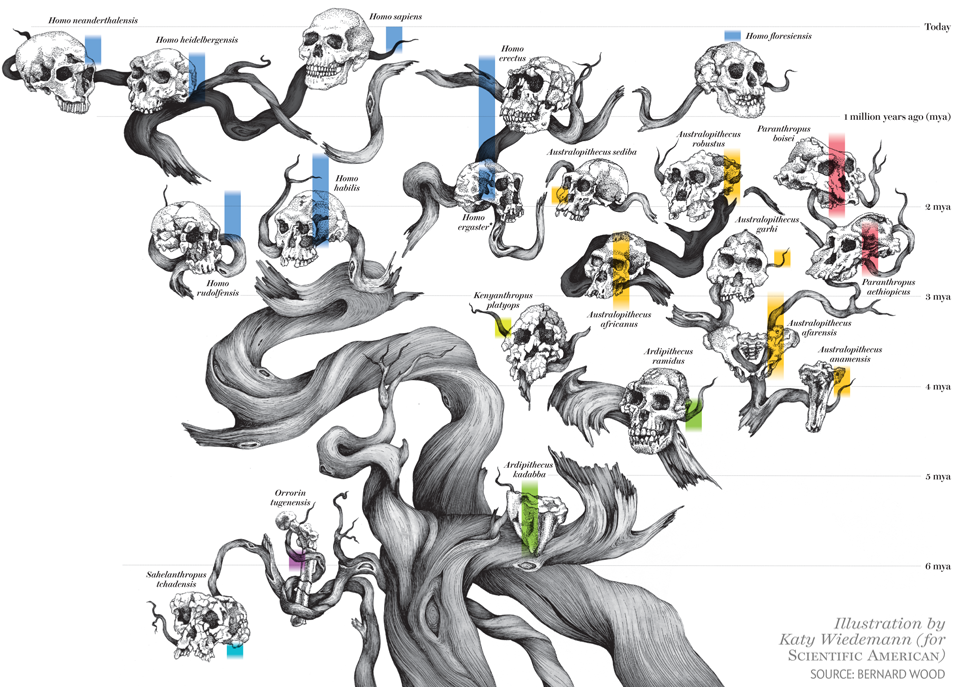
\includegraphics[width=\textwidth]{figures_c3/humanskulls.png}

        \caption{\textbf{The human family tree.} This is a visual depiction of the human lineage, starting with our common ancestorial roots. In \autoref{ch1}  it was shown that trees / graphs\protect\footnotemark are useful in showing relationships between items. Source: \citep{skull}}
        \label{fig:skulls}
\end{figure}
\footnotetext{A tree is a special case of a graph}



In the field of mathematics a graph, $G(\nu,\epsilon,\omega)$, is defined as a function of items (vertices\footnote{The term node, item or vertex shall be used interchangeably for the remainder of this chapter. This also applies to links/relationships/edges and edge-weight/strength}), $\nu$ which are connected through a series of connections (or edges$^1$) representing any relationships between them, $\epsilon$. Since relationships in the real world are rarely equivalent, we then encode the importance of each link in the form of an edge weight, or strength, $\omega$. Such formats allow both numerical and computational algorithms to understand and interpret the graph structure, providing us with information about the data or make use of automated layout programs for visualisation.


This chapter builds on the work shown in \autoref{ch2} - where
the ability to represent complex data in the form of a graph was used to (visually) draw information regarding network structure and temporal changes. Here situations, where the visual representation of many, large or complex networks is impractical, will be explored. We start by introducing a series of mathematical approaches which are capable of quantifying the graph (and nodes within it) and apply them to the co-author network for papers using the Master Chemical Mechanism (\autoref{sec:graphmetrics}). Following these global metrics are used to categorise the chemistry within different atmospheric chemistry mechanism subsets, and provide us with an insight to the chemistry structure (\autoref{sec:globalclass}) and finally apply these to real-world simulations representing a range of environments (marine, rainforest and urban) in \autoref{sec:metriccase}.
%
%
%

\section{Graph Metrics}\label{sec:graphmetrics}

The increase in the ability to gather useful data has resulted in difficulty when trying to interpret it (\autoref{sec:visbg}). The production of large, multivariate networks of inexplicable complexity hinders our ability to draw out meaningful conclusions based on visualisation alone. This means that much like the generation of mechanism \citep{protocol}, or creating semi-automated graph drawing layouts, we must rely on the field of mathematics coupled with computational aid (\autoref{ch2}).

Numerical algorithms derived from the field of Graph Theory can be used to circumvent the need for individual graph analysis and provide us with information about the network. One such subset of numerical algorithms are regarded as "centrality metrics", and may be used to rank the role and importance (centrality) of a node \citep{squaretower}. In the following sub-section, the four most common centrality metrics are discussed and applied to the MCM citation network.


\subsection{Centrality Metrics And Academic Publishing.}


One common application for graph analysis and visualisation is the representation and prediction of citation counts within academic journals \citep{cocite,google,naturecitation,netcoauthor}. Here network-visualisation techniques may be used to highlight the origins of a paper. For instance, \autoref{fig:naturecover} shows the multi-disciplinary research which underpins six prominent discoveries in the last 150 years.

The next section looks at the four most common centrality metrics and explores their properties with the use of an (approximate) citation graph showing the papers which cite the Master Chemical Mechanism (\autoref{sec:metricmcm}).



\subsection{The Master Chemical Mechanism (MCM)}\label{sec:metricmcm}

The MCM, \citep{mcm}, is a near explicit representation of our foremost understanding of gas-phase tropospheric chemistry. The mechanism describes the oxidation of 143 primary emitted VOCs and the respective rates at which this occurs. It has been tested on over 300 chamber experiments and used as a benchmarking mechanism to assist the development of reduced mechanism, providing a useful means for the evaluation of air quality models \citep{defra1}. The current version (3.3.1) contains 5809 chemical species and 17224 reactions to describe them \citep{isopmcm}. However there there are still a number of weaknesses that need to be considered. Firstly there very little \ce{Cl} chemistry and no other halogens in the mechanism. Reactions with \ce{O2} are implicit as are \ce{RO2}-\ce{RO2} reactions, which are shown through the reaction with an \ce{RO2} pool.





\subsection{Data Collection}\label{sec:scholar}

To generate a dataset on papers related to the MCM. The academic search engine (Google Scholar \citep{scholar}) is queried for all articles containing the words \{ \emph{"Master", "Chemical", "Mechanism"} and \emph{"MCM"} \}. For each match, the first 100 pages of results are selected. Each of these contains ten articles, from which the first 100 pages of related articles are chosen.
In taking the top 1000 citations for each page, a network of 15744 papers and 30178 citations\footnote{Note: this had the potential of returning up to 1000,000 nodes} is created. This process made use of an edited version of the  \emph{etudier} Github repository, \citep{web}.


\begin{figure}[H]
     \centering
         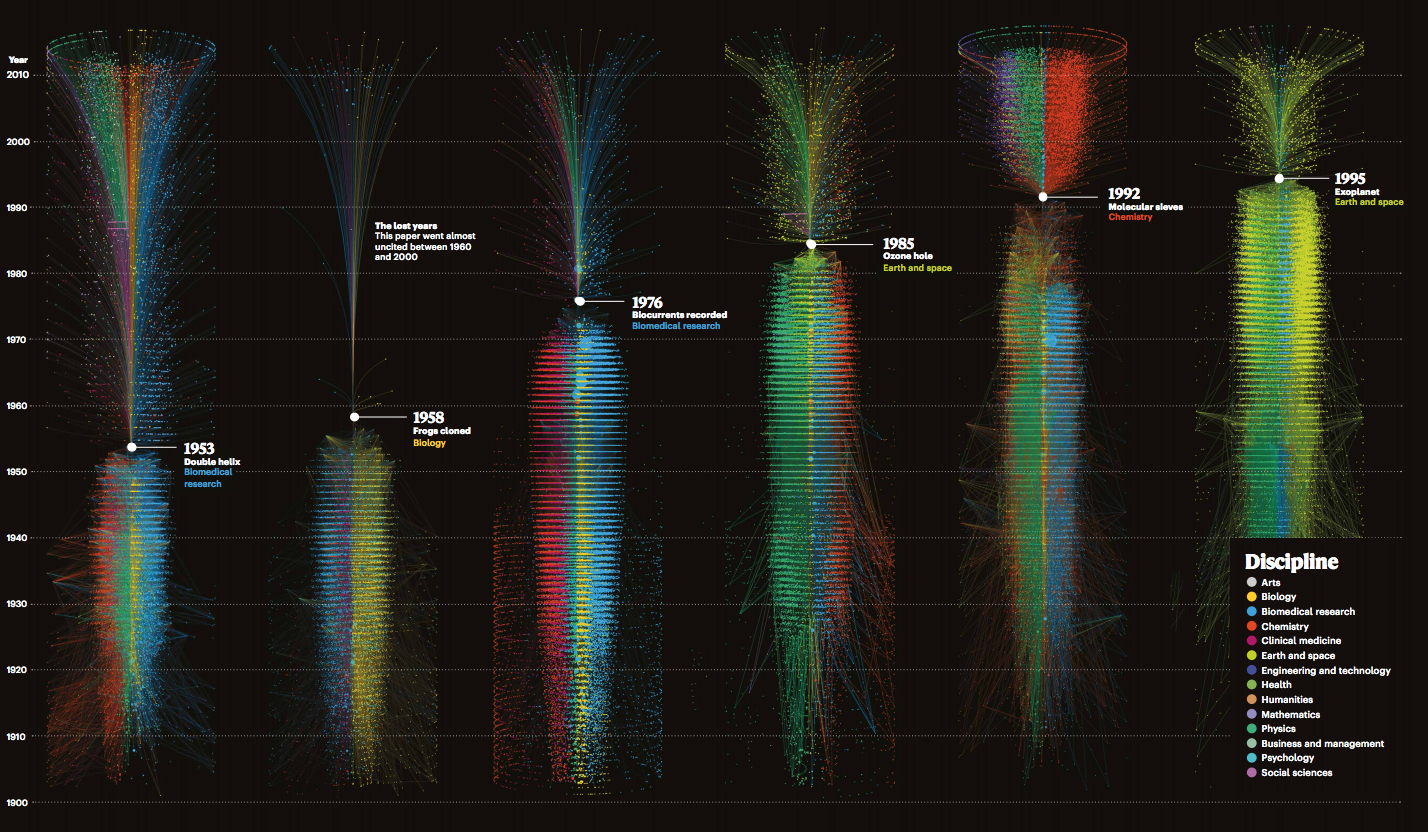
\includegraphics[width=0.92\textheight,angle=90]{figures_c3/naturegraph.png}

        \caption{\textbf{150 years of letters to Nature.} A visualisation showing how previous research is used to inspire future studies. Important discoveries (DNA, Cloning(frogs), Bio-Currents, Ozone Hole, Molecular Sieves and Exoplanets) are split into research which contributed to their formation (below), and the consequent papers produced from each discovery. Use of colour is used to emphasise the multi-disciplinary nature of prolific scientific discovery. Source: \citep{naturecover}}
        \label{fig:naturecover}
\end{figure}


\subsection{Visualising The Data.}

The initial visualisation of the dataset is accomplished through the use of THREE.js \citep{threejs}. This makes use of WebGL bindings and allows for the efficient viewing, querying and interacting of the data in 3 dimensions. This helped identify the temporal changes within the network by mapping a papers publication year to the $z$ direction, \autoref{fig:weball}, as discussed in \autoref{sec:filter3d}.

\begin{figure}[] %dont leave blank lines between sfig
     \centering
     \hfill
     \begin{subfigure}{0.495\textwidth}
         \centering
         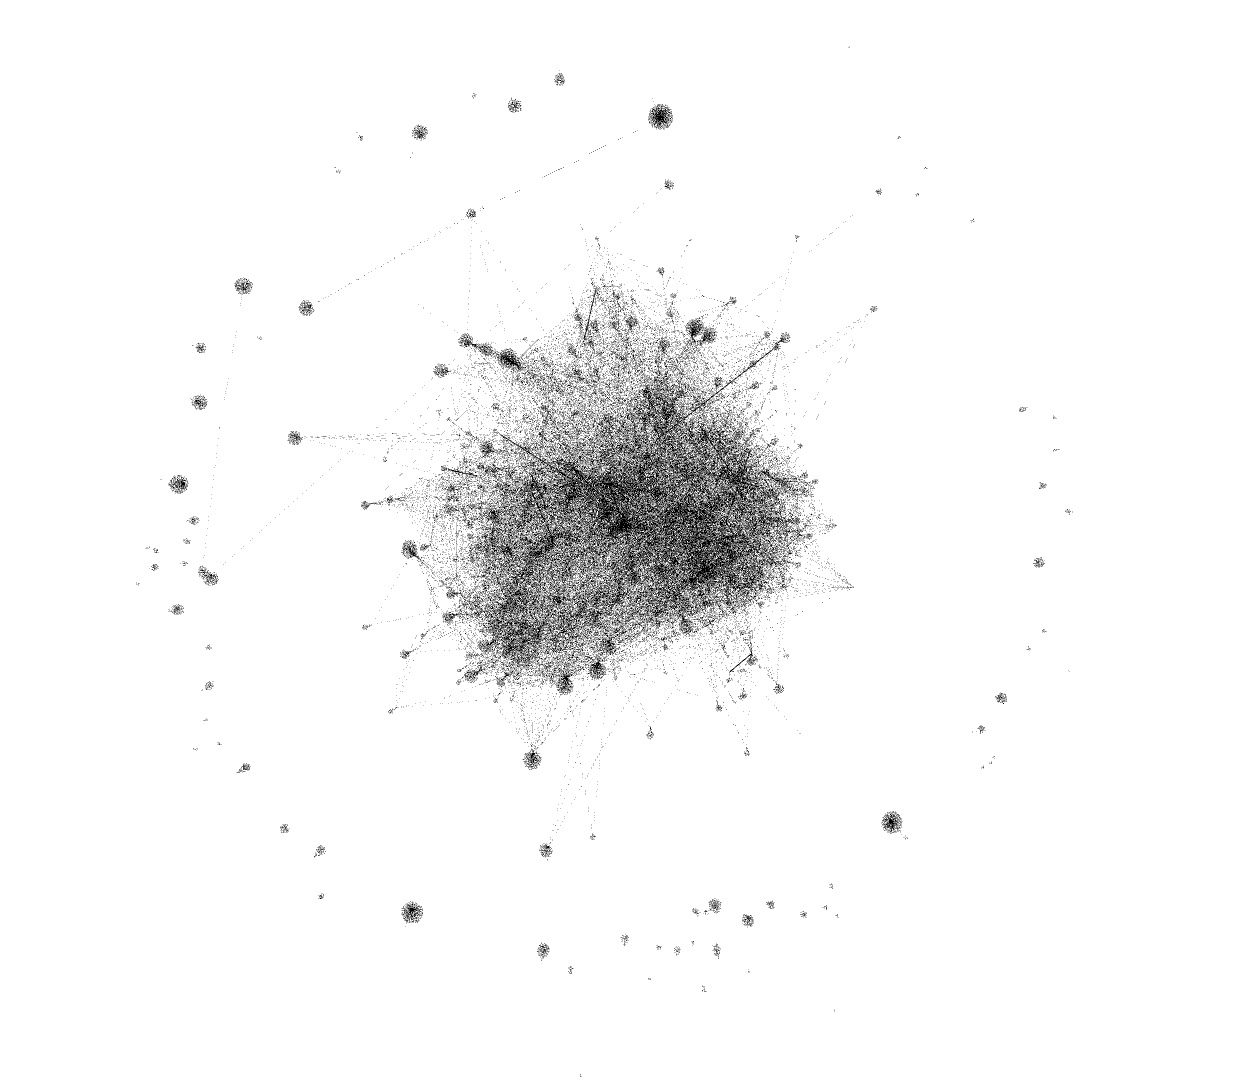
\includegraphics[width=\textwidth]{figures_c3/gephiall.png}
         \caption{A 2D force directed representation of the network using the gephi software \citep{gephi}}
         \label{fig:gall}
     \end{subfigure}
     \hfill
     \begin{subfigure}{0.47\textwidth}
         \centering
         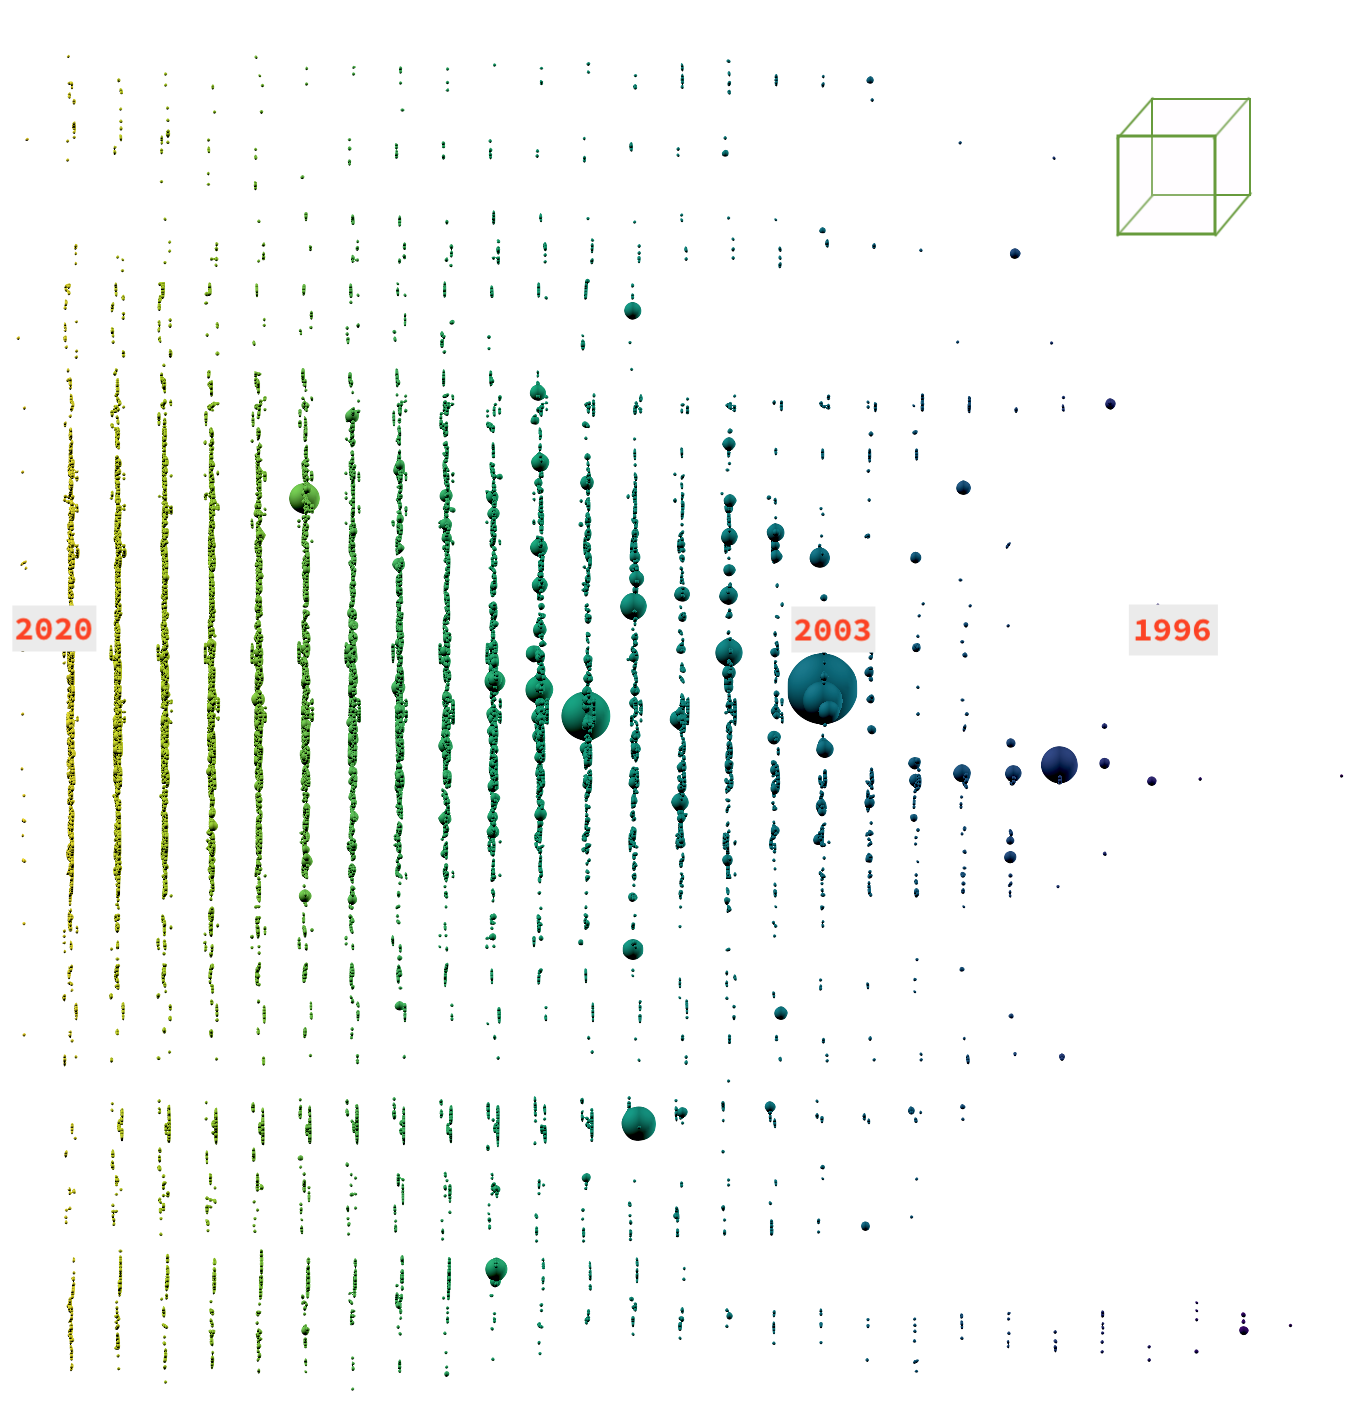
\includegraphics[width=\textwidth]{figures_c3/sideall.png}
         \caption{3D orthographic camera (sideview). This shows a sideways view of the graph in (a) where time is across the $x$ axis }
         \label{fig:sideweb}
     \end{subfigure}
     \hfill

     \begin{subfigure}[b]{0.75\textwidth}
         \centering
         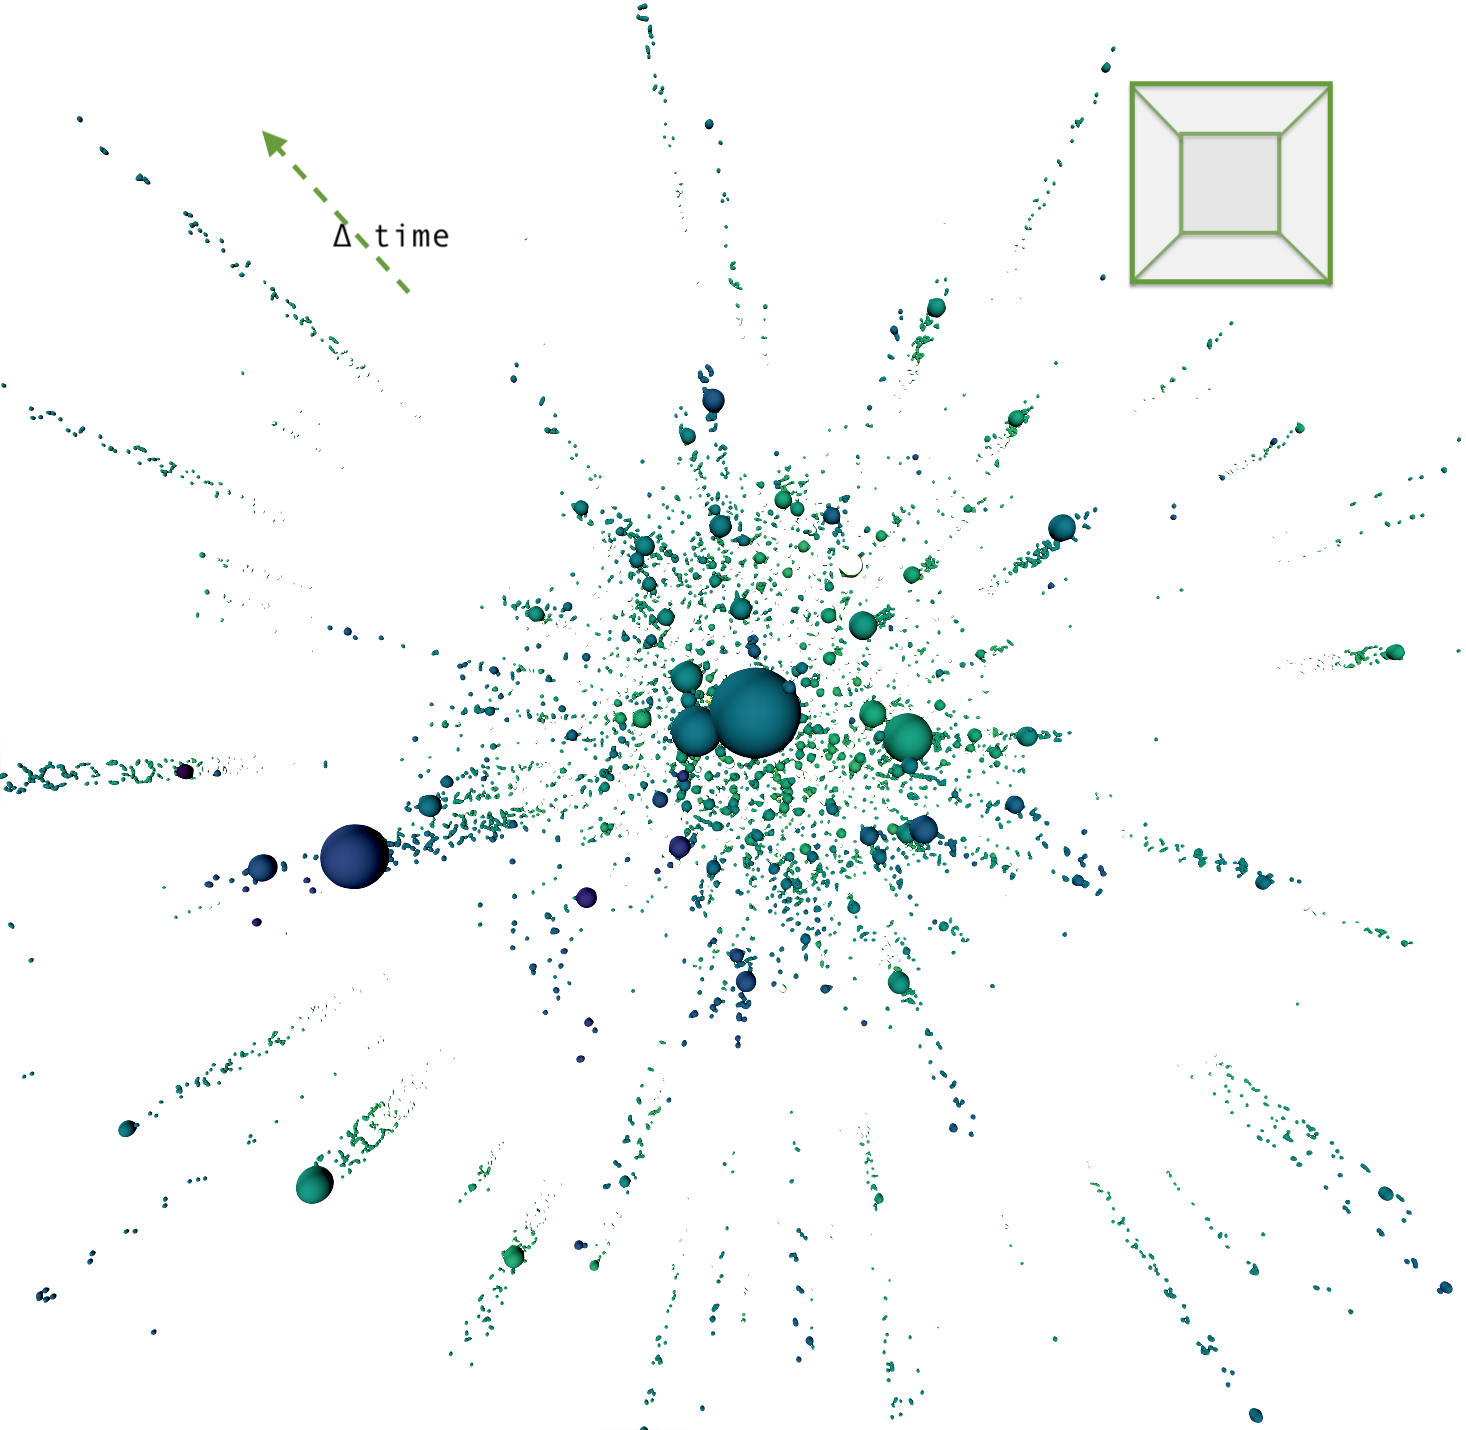
\includegraphics[width=\textwidth]{figures_c3/threeall.png}
         \caption{3D perspective camera}
         \label{fig:3dgeph}
     \end{subfigure}


        \caption{ \textbf{Initial 3D graph representation of the scraped MCM citation graph.} (a) shows the `classic' graph representation of the network. (b) shows a size representation using an orthographic perspective. Here time is shown across the $x$ axis, with yellow being the most recent. (c)
        uses a perspective camera, which emphasises the time component of the data.
        Still captures of 2D and 3D visualisations of the dataset.\\
         \textbf{Node size} corresponds to the number of citations, and colour (and z-axis) corresponds to the publication year for each paper.}
        \label{fig:weball}

\end{figure}


\subsection{Filtering The Data}\label{sec:filter3d}


In the method used to web scrape data, there are several features which need to be corrected/removed. The reasons for this are discussed below.


\textbf{A note on unintentional filtering}\\
\textit{
The script used for web scraping extracts author names directly from the google scholar page, and not the articles themselves. This means some author names can be omitted and replaced by ellipses - producing an inaccurate graph. Therefore the results in this section are not explicit, but rather a demonstration of graph theory on a real-world dataset.
}


\paragraph*{Pre-1996}
There exist several papers predating the conception of the MCM (1996). A number of these are incorrect and contain publication dates <1900 which may be the result of missing information or a fault in googles web scraping algorithm. Any such papers are removed from the dataset.

Articles published before 1996 are deemed necessary in the creation of the MCM, but not its influence on the field of atmospheric science ( see cone shape in \autoref{fig:sideweb}) - it, therefore, makes sense to filter these from the dataset.


\paragraph*{N-th degree research}
Not all research articles in a field reference other articles with the same field. \autoref{fig:naturecover} showed us that many of the great discoveries in science have a multi-disciplinary nature. It is for this reason that it is expected that articles from non-atmospheric areas of research may reference or build upon specific areas of research touched by the MCM. Such papers, and in consequence the papers which cite them, have little or no links to many of the core MCM papers. Such papers manifest themselves as a halo of satellite clusters which are connected by themselves but not with the main body of the graph, \autoref{fig:gall}. In using a 3D perspective viewpoint (\autoref{fig:3dgeph}) it is possible to identify the paper which references the MCM and then the consequent papers which cite it by observing the satellite clusters, and the gradually lightening spiral of papers which emanate out of it. These groups of papers are now discussed.

Analysis of the network connections for each cluster can allow us to identify the indirect relationships between some of these diverse topics (\autoref{table:otherpapers}) contained within the satellite nodes. Here it can be seen that the use of photochemical ozone creation potentials \citep{milk1,milk2} are used for the Life cycle assessment of Italian high-quality milk production \citep{milk}.
Similarly, indirect paths such as the paper:
 "Temporal controls on dissolved organic matter and lignin biogeochemistry in a pristine tropical river" (\citep{biogeo}) can be used to link to \citep{georiver1} and ultimately the MCM protocol paper \citep{mcmpartA}.

 If we desired to remove such papers, the simplest method would be to recreate the graph into one where links are drawn between papers that are cited together (\autoref{sec:cocitep})
 and then removing any nodes without any external connections (isolates).

\begin{table}[H]
\begin{center}
\begin{tabular}{ p{0.6\textwidth}|l }
 \hline
   & \\
 Fabrication of Bioinspired Actuated Nanostructures with Arbitrary Geometry and Stiffness & \citep{nano} \\ \\
 %
 Temporal controls on dissolved organic matter and lignin biogeochemistry in a pristine tropical river  & \citep{biogeo} \\ \\
Neuroproteomics in Neurotrauma & \citep{neurotrauma}\\ \\
%
Fast start-up of a pilot-scale deammonification sequencing batch reactor from an activated sludge inoculum & \citep{pilot} \\ \\
Red blood cell oxidative stress impairs oxygen  delivery and induces red blood cell aging & \citep{blood} \\ \\
%
Life cycle assessment of Italian high quality milk production. & \citep{milk}\\ \\
%
 \hline
\end{tabular}
\end{center}

\caption{A selection of research papers not directly connected to the field of atmospheric modelling.}
\label{table:otherpapers}
\end{table}



\paragraph*{Unprobable occurances}
Finally, the extracted network also contains many disconnected component subgraphs - graphs with no connection to atmospheric science. An example of this is seen in an article about neuroproteomics in neurotrauma \citep{neurotrauma}. In analysing the paths which connect this, it is seen to cite the paper on "Large scale gene expression profiling of metabolic shift of mammalian cells in culture", \citep{neuro2}. This is an anomaly which within its structure contains the words "Master", "Chemical" and "Mechanism" (separately) and has `MCM' as an abbreviation for one of the author names. Disconnected sub-components are omitted from the analysis to remove such papers.





\subsection{The Co-Citation Network}\label{sec:cocitep}

The document coupling techniques of co-citation was introduced in the 1970s as an alternative approach for quantifying the results within the science citation index \citep{cocite}. Rather than representing a graph using backpropagation (through the use of referencing and citation counts), a co-citation network introduces a link between papers if, and only if, they have been cited together. Although this loses the directionality of a graph, it allows us to show forward propagating trends between papers within the same field.

Applying the above method allows us to reduce the citation graph of 451 papers and 5402 edges to an undirected co-citation graph of 2758 edges - halving the number of original links between papers.

\subsection{The Co-Authorship Network}
An alternative to exploring which papers which are cited together are to look at their authors. Here undirected links are drawn between authors on the same paper. This style of analysis was used to show that the number of papers per author, and the total number of authors per paper can vary between research fields, \citep{newmancoauthor}. In combining this with a series of network centrality metrics, \citep{coauthornew} revealed that it is possible to discern promising researchers from both iter and Intra disciplinary groups.

In building a co-authorship network for the MCM, we can identify authors who publish together\footnote{ Disclaimer: as mentioned earlier, not all authors for every paper were recorded by the web scraping algorithm} and highlight research groups who work with the MCM, \autoref{fig:authorgroup}. This shows how authors with a similar geographic location/institution are more likely to publish together. The largest cluster here falls under the MCM developer team, which resides between the University of Leeds and York. Next two German institutions which are heavily involved in the atmospheric chemistry field (FZ-Julich and Max Planck for Chemistry, Mainz), followed by an assortment of Chinese authors, mainly centred around the Beijing or Hong Kong region.


\begin{figure}[H]
     \centering
         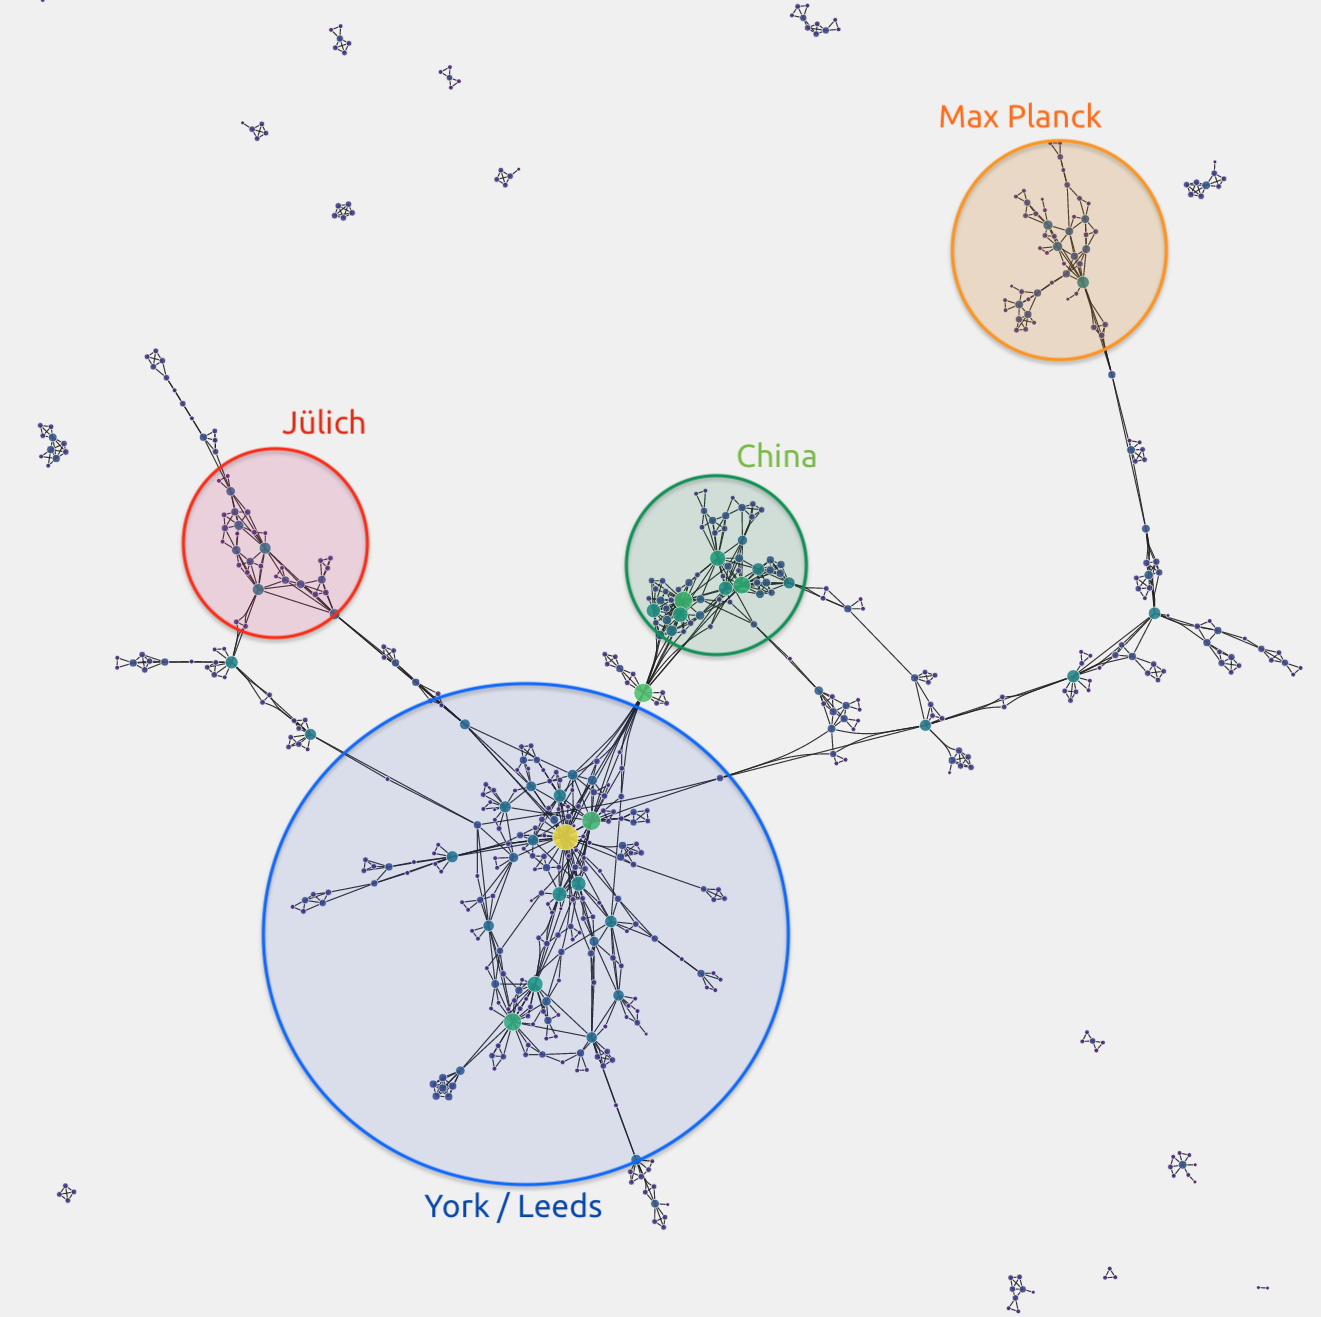
\includegraphics[width=.8\textwidth]{figures_c3/GroupAuthor.png}
        \caption{ \textbf{The co-author network.} In representing the authorship network as a force-directed graph, we see cliques or clusters of people who publish together. It is noted that this often occurs when they have a similar geographical location. Node sizes and colour represent author rankings using the PageRank algorithm (\autoref{sec:pagerank})}
        \label{fig:authorgroup}
\end{figure}


\textbf{Labeled Graph of \autoref{fig:authorgroup}}\\
\textit{See \autoref{appendix:fullauthor} for a heavily labelled version of the graph above graph showing the co-author network on work relating the Master Chemical Mechanism. }


\section{Metric Analysis}\label{sec:graphcentrality}

The co-author network (\autoref{fig:authorgroup}) can be used to demonstrate the functions of each centrality metric. This subsection will access the efficiency of graph centrality metrics in their ability to identify influential nodes within a network.

\newpage

\subsection{Degree Centrality}
The simplest, and most intuitive, metric is degree centrality \citep{degreefreeman}.  In counting the number of edges incident on a node (in and out), we calculate the degree of a node. In this instance, this corresponds to the number of papers co-authored by an individual. This gives us an idea of the importance of a node and has been used to calculate influence within social media or the probability of a profile committing online auction fraud \citep{degreetwitter,degreefreeman}.


\begin{quote}
\textit{
\textbf{Example analogy:} If we take the UK rail network as an example, As individual stations, Warrington, Birmingham, Manchester and Doncaster all have a high degree (a large number of different rail networks passing through them. Similarly for the London network, Victoria and Kings Cross will have the highest degree value.). Examples are shown in \autoref{appendix:rail}
}
\end{quote}

The author network in \autoref{fig:degauth} shows many of the names with a high degree are contributors (or colleagues to the contributors) of the MCM at Leeds. The authors with the most collaborations, or links, are very likely to appear within the most cited or citing papers (\autoref{tab:In-Degree_Citation} and \autoref{tab:Out-Degree_Citation} discussed below). This is likely because both development (well-cited) and the evaluation/usage (well citing) of a mechanism requires knowledge from a range of different fields, making it an interactively collaborative process.

\begin{figure}[H]
     \centering
         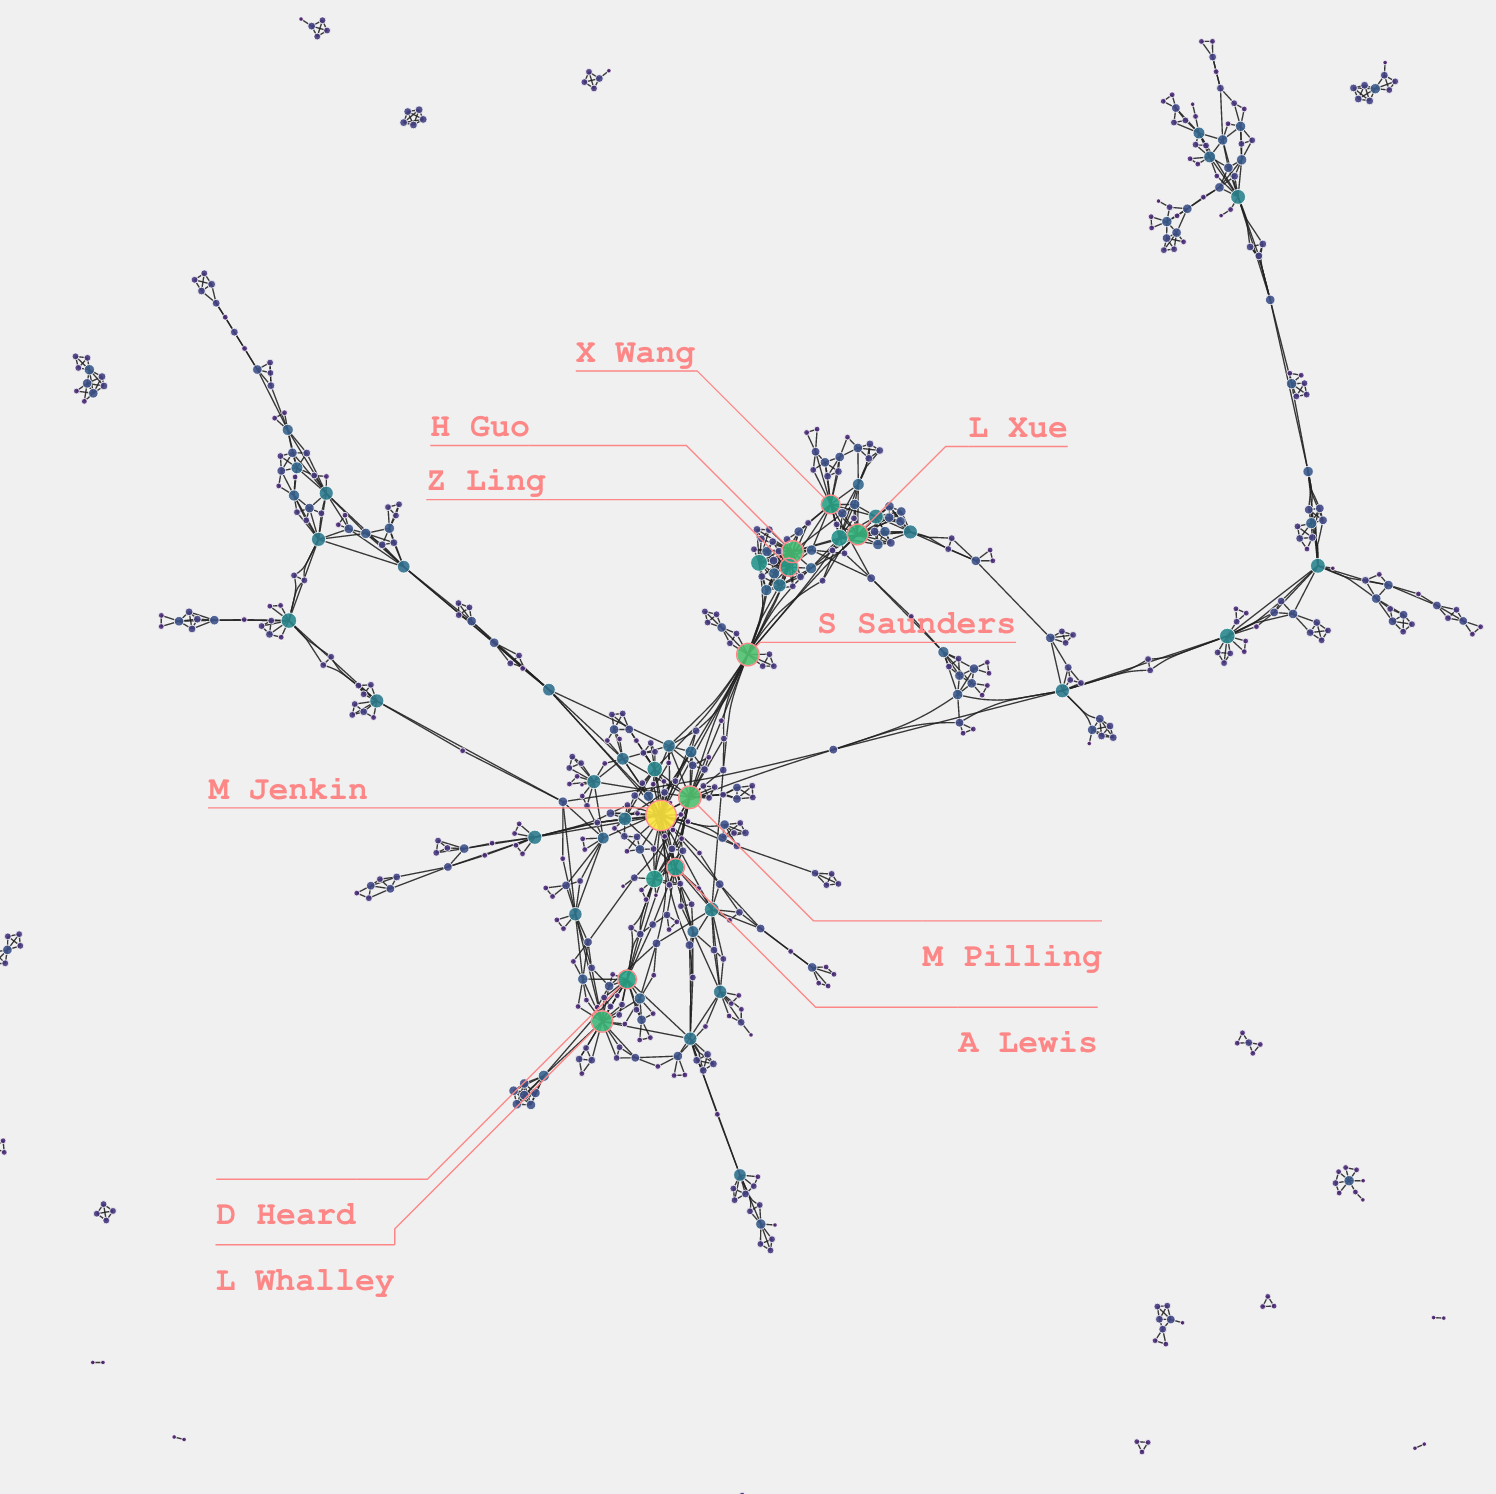
\includegraphics[width=.8\textwidth]{figures_c3/degreeauthor.png}
         \begin{table}[H] \centering\begin{tabular}{lr}
\toprule
   \hphantom{ } M Jenkin &  39 \\
 \hphantom{ } S Saunders &  25 \\
  \hphantom{ } M Pilling &  25 \\
      \hphantom{ } H Guo &  24 \\
  \hphantom{ } L Whalley &  23 \\
      \hphantom{ } L Xue &  22 \\
    \hphantom{ } D Heard &  19 \\
     \hphantom{ } X Wang &  19 \\
     \hphantom{ } Z Ling &  18 \\
    \hphantom{ } A Lewis &  17 \\
\bottomrule
\end{tabular}
    \label{tab:degree_Author}
    % \caption{\textbf{Author network}: Top 10 ranked items using degree centrality}
    \end{table}

    
        \caption{ \textbf{Degree Centrality.} In applying the degree centrality to the co-authorship network, it is possible to pick the authors with the greatest number of papers, of which the top 10 have been listed.}
        \label{fig:degauth}
\end{figure}

\subsubsection*{Directed Degree}
For graphs where link direction holds an inherent meaning regarding their representation (for example in the citation graph an outward link symbolises that paper citing the one that the link points to), it is possible to further divide the degree centrality metric into inwards and outward links. This can allow us to separate authors who are highly cited (in-degree) from those who use lots of papers (out-degree). In applying these metrics to the directed citation graph, it is possible to get an insight into the core MCM development papers (\autoref{tab:In-Degree_Citation}) and separate them from those who make use of the mechanism as part of a greater study (\autoref{tab:Out-Degree_Citation}).
\begin{table}[H]
    \centering
     \begin{tabular}{p{0.6\textwidth}r}
     \toprule
      & \\ \\
     Protocol for the development of the Master Chemical Mechanism, MCM v3 Part A tropospheric degradation of nonaromatic volatile organic compounds & \cite{mcmpartA}   \\ \\
        Protocol for the development of the Master Chemical Mechanism, MCM v3 Part B tropospheric degradation of aromatic volatile organic compounds & \cite{mcmpartB}   \\ \\
        Development of a detailed chemical mechanism MCMv3. 1 for the atmospheric oxidation of aromatic hydrocarbons & \cite{detailedmcm}   \\ \\
        \bottomrule
    \end{tabular}
    \caption{\textbf{In-Degree of the citation network}: The top 3 most cited papers.}
    \label{tab:In-Degree_Citation}
    \end{table}

    
\begin{table}[H]
    \centering
     \begin{tabular}{p{0.6\textwidth}r}
     \toprule
      & \\ \\
     The MCM v3.3.1 degradation scheme for isoprene & \cite{isopmcm}  \\ \\
        Atmospheric photochemical reactivity and ozone production at two sites in Hong Kong Application of a master chemical mechanismphotochemical box model & \cite{hongkongmcm}   \\ \\
        HOx budgets during HOxComp A case study of HOx chemistry under NOxlimited conditions & \cite{hoxcompmcm}  \\ \\
        \bottomrule
    \end{tabular}
    \caption{\textbf{Out-Degree of the citation network}: The top 3 most citing papers.}
    \label{tab:Out-Degree_Citation}
    \end{table}

    


\subsection{Closeness Centrality}\label{sec:closeness}
Often within a network, we are interested in how easy it is to to get information from one node to every other node. This is what the closeness centrality tells us. To calculate a nodes closeness, we begin by taking the reciprocal sum of all the Dijkstra paths\footnote{The shortest available path.} to every other node \citep{closeness-book,closeness}.
This gives a representation of how far information from a particular person (node) will need to travel to reach every other node. Such a metric has applications in intelligence gathering, telecommunications and word importance within key-phrase extraction \citep{terror,examples_centrality,phrase}.

\begin{quote}
\textit{
\textbf{Example analogy:} If we take the UK rail network as an example, York station will have a high closeness value as it is well connected and central in location. This means it is easy to reach every other location when compared to other stations, \autoref{appendix:rail}
}
\end{quote}

For the co-authorship network, \autoref{fig:closeauth}, nodes have been coloured by their closeness value. Here a heat-map-like effect may be observed, showing that information between the dense Leeds-York cluster makes it easier to disseminate information across all parts of the graph. The results of the closeness centrality suggest that if a problem (bug), or improvement (update) occurs, Michael Pilling would be the best served to pass that information to all other groups using the MCM.

\begin{figure}[H]
     \centering
         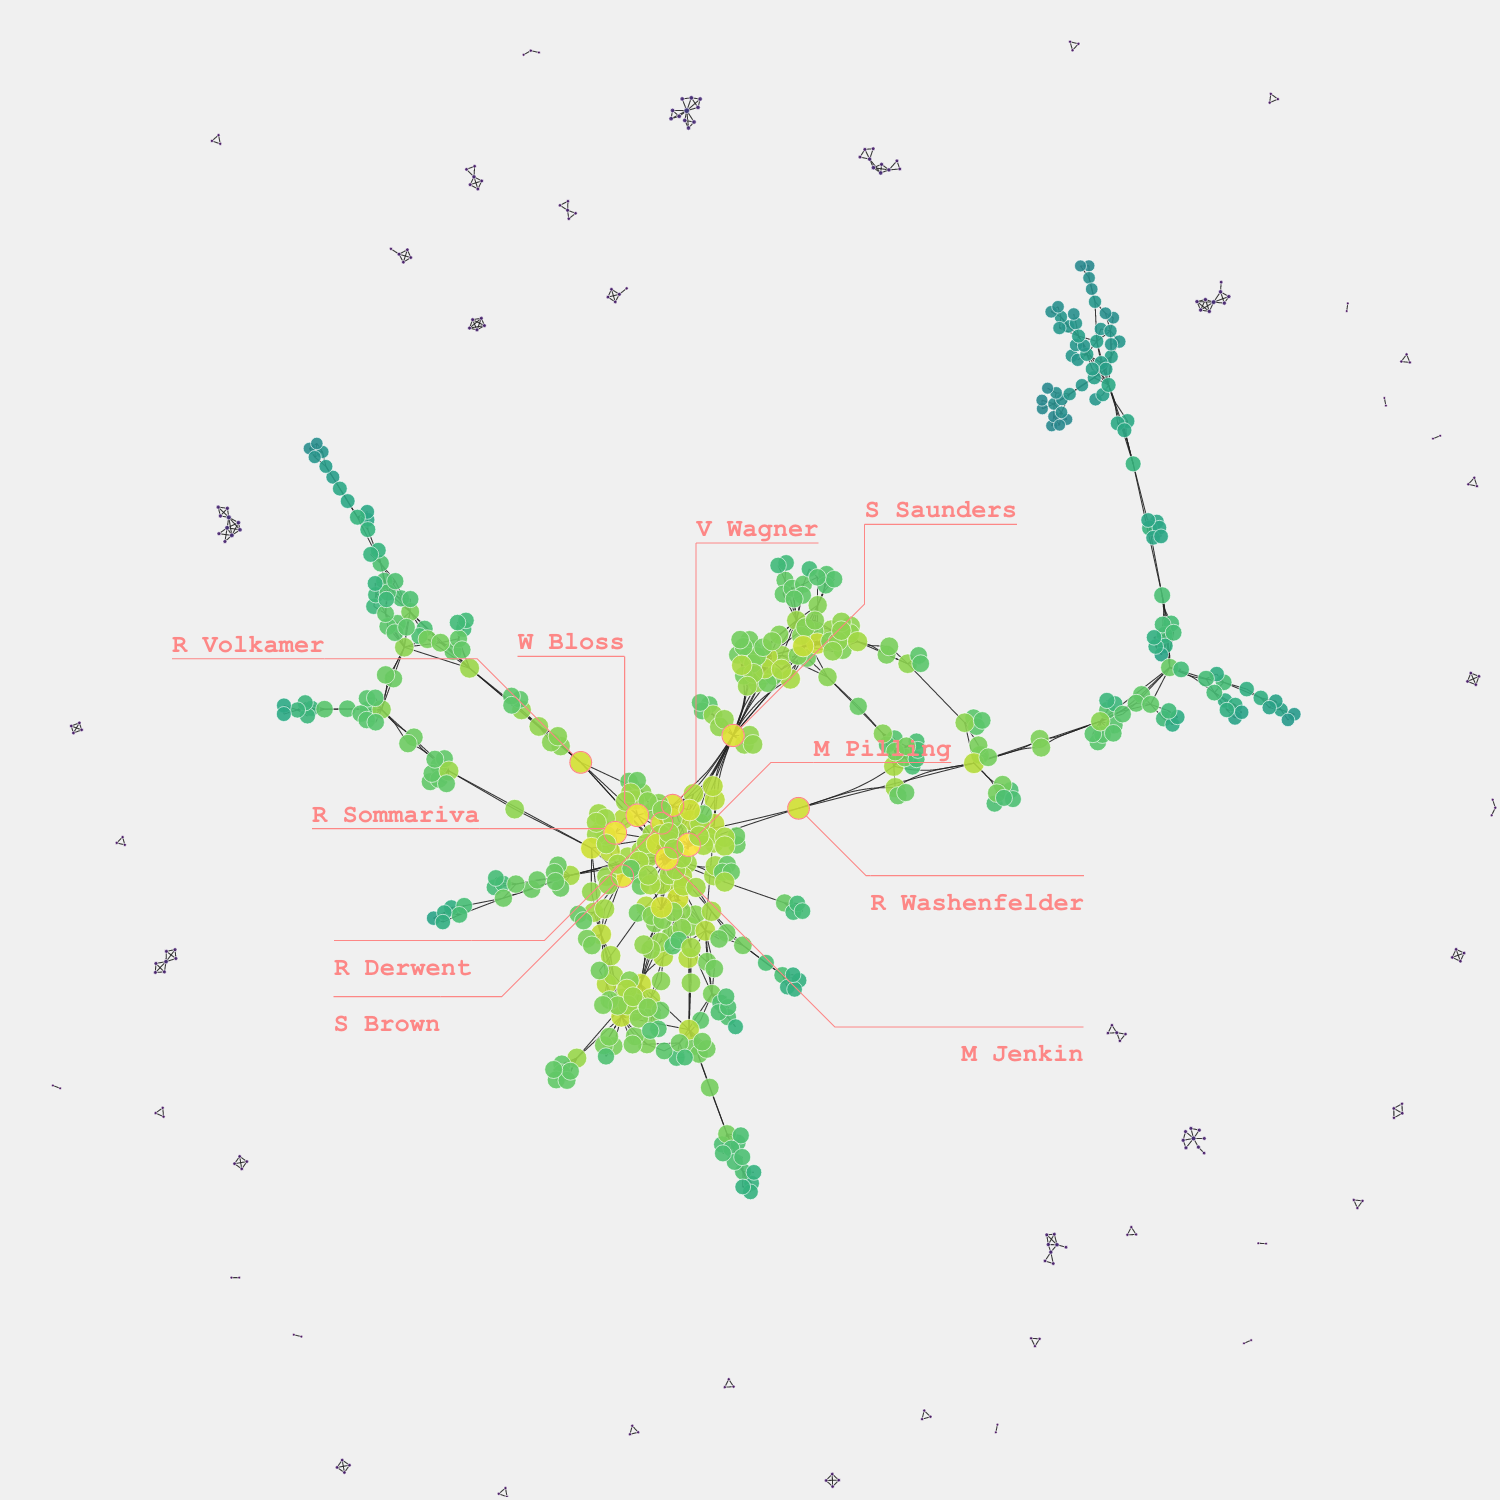
\includegraphics[width=.8\textwidth]{figures_c3/closenessauthor.png}

         \begin{table}[H] \centering\begin{tabular}{lr}
\toprule
      \hphantom{ } M Pilling &  0.149995 \\
       \hphantom{ } M Jenkin &  0.146532 \\
    \hphantom{ } R Sommariva &  0.145251 \\
        \hphantom{ } W Bloss &  0.144052 \\
        \hphantom{ } S Brown &  0.142059 \\
     \hphantom{ } S Saunders &  0.140176 \\
       \hphantom{ } V Wagner &  0.139281 \\
      \hphantom{ } R Derwent &  0.136450 \\
     \hphantom{ } R Volkamer &  0.136184 \\
 \hphantom{ } R Washenfelder &  0.135918 \\
\bottomrule
\end{tabular}

    \label{tab:closeness_Author}
    % \caption{\textbf{Author network}: Top 10 ranked items using closeness centrality}
    \end{table}

    
        \caption{ \textbf{Closeness centrality within the co-Author network.} Here a colour/size gradient is seen, with the nodes that are more central (in location) and better connected having a higher closeness than those in the peripheries - which are harder to get to.}
        \label{fig:closeauth}
\end{figure}
%
\subsection{Betweenness}\label{sec:betweenness}
In social networks, it is often important not only to know who has the greatest reach (closeness centrality) but also where bottlenecks or `broker' positions occur. Nodes with a high betweenness control, or limit, the amount of information that can be transferred across the network. If a node lies on a geodesic (the shortest path between two other nodes), we may consider it a `pivotal' node, due to its role within the network \citep{neoj4}. Should such a node then be removed, the overall flow of information incurs either a deviation, the information will either need to travel a longer (alternative) route or may not be able to reach its destination at all \citep{betweenness, between, betweenfast,examples_centrality}.
Betweenness centrality is a count of the number of geodesics which pass through a node. If multiple `shortest' paths are possible, these can be accounted for using division in the algorithm mathematics.


\begin{quote}
\textit{
\textbf{Example analogy:} Expanding on the UK rail network analogy, Shrewsbury station serves the critical role of connecting many lines from England to Wales. In removing this station, routes from the Liverpool or Manchester to Cardiff will be greatly increased. Additionally, the Aberystwyth section of the line will then become isolated from the rest of the country.
}
\end{quote}

Authors with a high betweenness in \autoref{fig:betauth} are seen to lie along the joints between clusters. Here we can imagine that removing Li, Griffin or Liu can disrupt the overall flow of collaboration, potentially isolating the work of the Max Planck for Chemistry from that of everyone else. Similarly, Jenkin and Pilling can be seen as holding much of the Leeds cluster together. In removing them from the network (if for example, the refused to collaborate) it is possible to see how many of groups within the Leeds environment may not have worked together, with the cluster potentially separating into several smaller groups. Finally, we see that Saunders (Australia) is highlightes as an important node - an action which can be attibuted her introducing the Chinese atmospheric community to the MCM. In removing her from the network, it can be seen that much of the collaboration which exists would have been significantly less likely.

\begin{figure}[H]
     \centering
         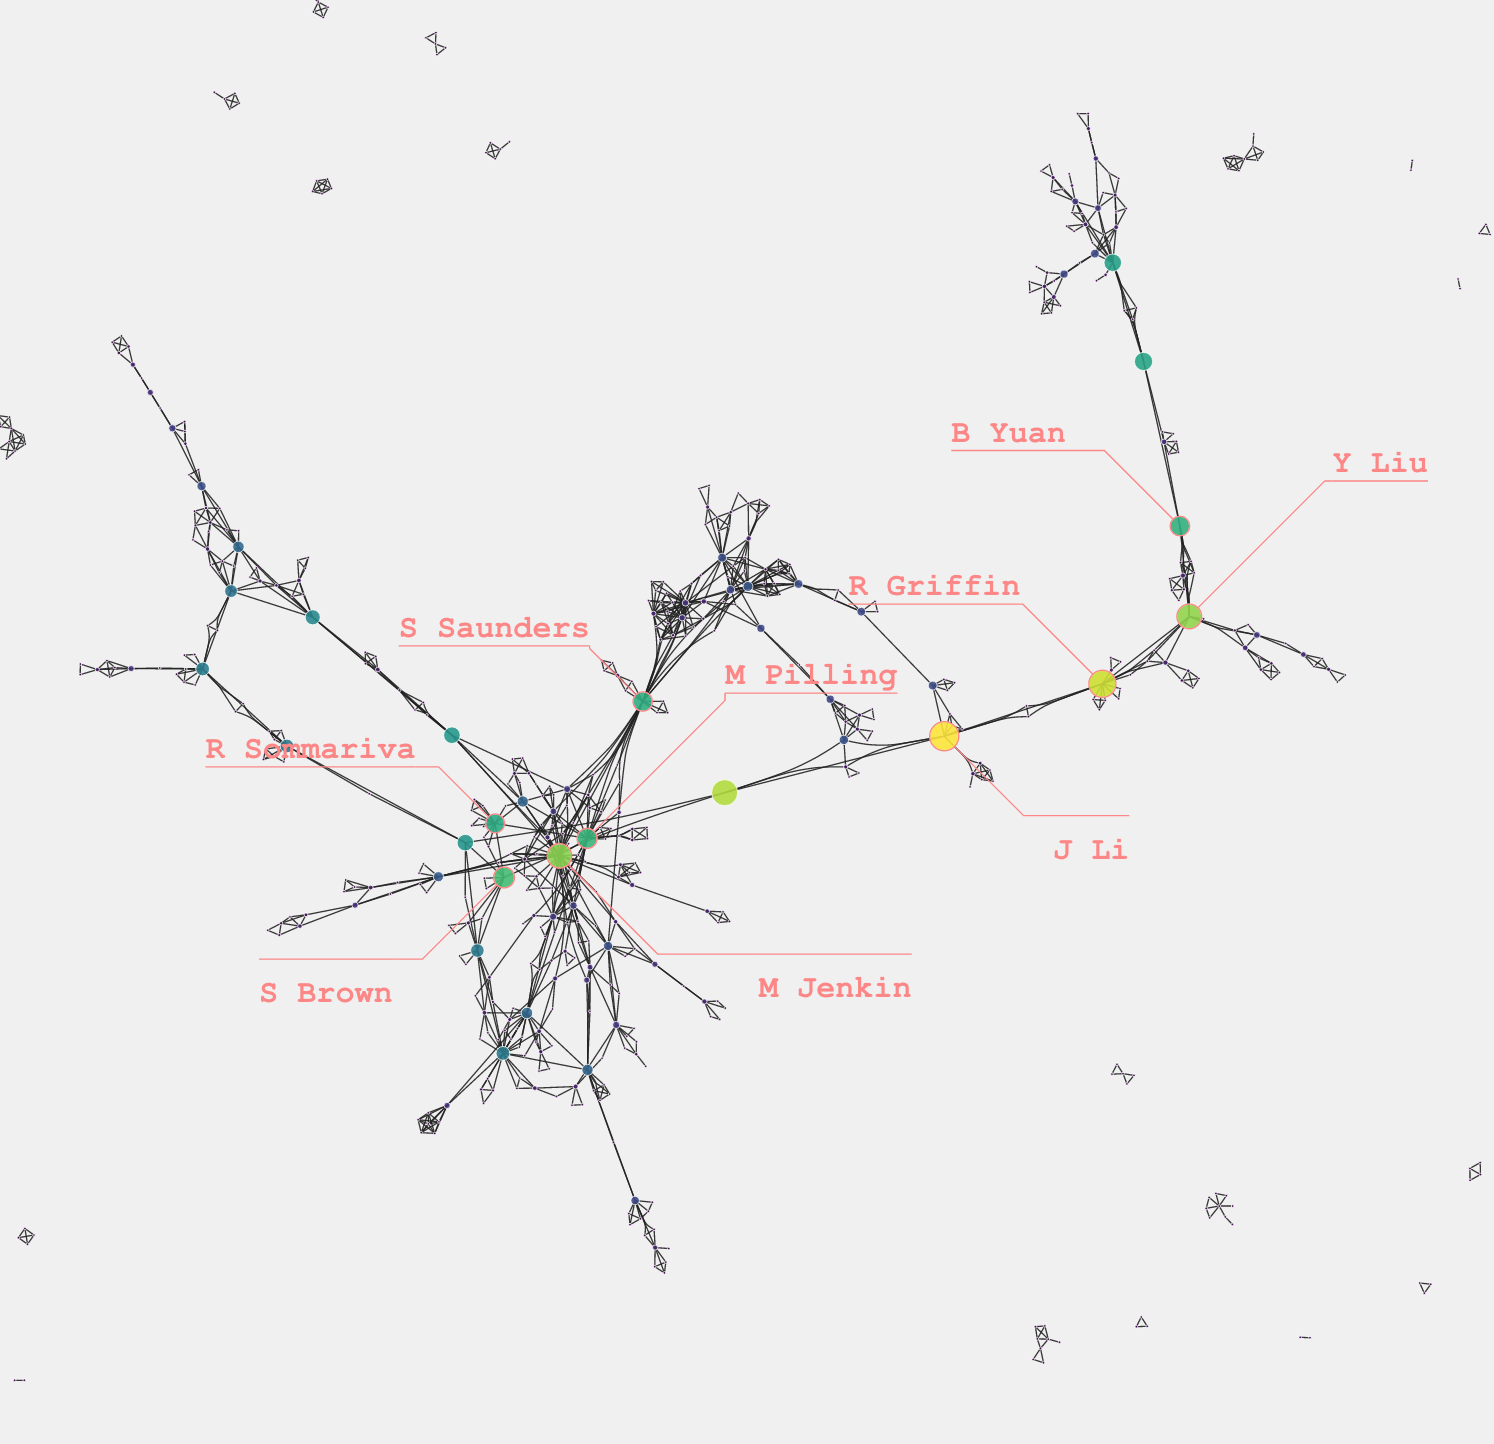
\includegraphics[width=.8\textwidth]{figures_c3/betweenauthor.png}
         \begin{table}[H] \centering\begin{tabular}{lr}
\toprule
           \hphantom{ } J Li &  0.180998 \\
      \hphantom{ } R Griffin &  0.162558 \\
 \hphantom{ } R Washenfelder &  0.153024 \\
          \hphantom{ } Y Liu &  0.142194 \\
       \hphantom{ } M Jenkin &  0.139818 \\
        \hphantom{ } S Brown &  0.110188 \\
      \hphantom{ } M Pilling &  0.102816 \\
         \hphantom{ } B Yuan &  0.099914 \\
     \hphantom{ } S Saunders &  0.097255 \\
    \hphantom{ } R Sommariva &  0.094757 \\
\bottomrule
\end{tabular}

    \label{tab:betweenness_Author}
    % \caption{\textbf{Author network}: Top 10 ranked items using betweenness centrality}
    \end{table}

    
        \caption{ \textbf{Betweenness centrality within the co-Author network.} Nodes which lie on a pivotal position (connecting/bottleneck) tend to have a high betweenness value due to their crutial role within the network. The colour represents the betweenness centrality}
        \label{fig:betauth}
\end{figure}


%
\subsection{Spectral Methods And Matrix Analysis}

Graphs can often be represented in the form of relationship (adjacency) matrixes (ref Chapter 1). This allows us to apply the theory of linear maps, such as eigenvectors and values, to stochiometric data in matrix form. Such methods have been around since the 1950s, \citep{seeley}, but mainly became popular with the release of Larry Page's page-rank algorithm \citep{google} - the algorithm that began google. These methods, in addition to the HITS algorithm (\autoref{hits}), make use of a graphs native matrix representation to calculate node importance. Spectral algorithms can be broken down into four categories \citep{spectral}:

\begin{table}[H]
  \centering
\begin{tabular}{p{.22\textwidth}||p{.34\textwidth}| p{.34\textwidth}}
\hline
 & No Normalisation  & Row Normalisation \\
 \hline \hline
No Damping & Eigenvector \citep{eigen, eigen2}  \: & Markov Chain Steady State \citep{seeley} \: \\ \hline
Damping & Katz \citep{katz} \: & Total Effect Centrality PageRank \citep{google} \\ \hline
\end{tabular}
\end{table}


Here damping terms represent the probability of moving to the new random starting position, allowing for the user to `randomly select a new webpage' or leave an isolated cluster. The normalisation of the matrix does not affect the node ranking, but merely adjusts the numerical output of the algorithm. It is for this reason that its overall practicality may be debated \citep{spectral}. Since page rank is the most common of these methods and allows for a tune-able degree of randomness within network propagation, this is discussed in more detail in the next subsection.



    \paragraph*{Hypertext Induced Topic Search (HITS)}\label{hits}
    A common eigenvector algorithm used for classifying webpages is the
    HITS algorithm. This helps categorise the role of a node as either a Hub or an Authority,
     \citep{hits,hitsvspagerank,hitsweb}. Similar to the in and out-degree metrics, this algorithm separates nodes with many outgoing links (an authority) from those with many ingoing ones (an information hub). Overall this provides similar results to the in/out-degree, although since it looks more on how information propagates across the network as a whole, it often provides more accurate, and different, rankings to simple degree analysis.






\subsection{Page Rank}\label{sec:pagerank}
Arguably the best-known centrality algorithm is PageRank. This is a spectral method for measuring the transitive influence of a node, by taking the effect of neighbours and by their neighbours into account \citep{neoj4}. The page rank algorithm was initially developed to provide a better way of ranking web pages \citep{google}. Here an important page is not only one of many links, but links to other important sources. In the context of academic papers, that same paper also found that in predicting future citations, the page rank algorithm fared better than using the current citation count of a paper.
To explain how this works, we will look at the mathematics behind the algorithm, and then eventually apply it to the co-authorship graph in \autoref{sec:applypr}

\subsubsection{The Google Matrix}
To solve for page rank, a `google matrix' must first be constructed. Once done this is iterated until convergence is reached.

To build a google matrix, we must first generate a dyadic link map of the graph\footnote{In sociology a dyad is a group of two people - the smallest possible social group.} - its adjacency matrix $A_{i,j}$ ($i,j$ are the source target indexes). This is then converted into a Markov matrix $M_{i.j}$ by dividing each column $j$ by the sum of the total outgoing links of node $j$, Algorithm \ref{eqn:markov}.
Items with no outgoing links (sinks), are adjusted with either a personalised\footnote{The use of user chosen (beginning) values for each node are used.} list of values or the constant $1/n$, (where $n$ is the number of nodes) to replace the zero-sum columns. This produces a normalised\footnote{ \: $\Sigma_{i=1,n} M(i,j) = $ unity} matrix of Markov chains representing the fractional production for node $j$ from all other nodes.

\begin{algorithm} \caption{Adjacency to Markov matrix.}
\begin{algorithmic}[1]
\State Obtain graph adjacency matrix, $A_{i,j}$.
\Repeat
\ForEach{$ j \in \mathcal{}$ columns}
\State $M($:$,j) \gets A($:$,j) / \Sigma_{i=1,n} A(j,i)$
\EndFor
\Until {$\Sigma_{i=1,n} M(i,j) = 1$}

\end{algorithmic}\label{eqn:markov}
\end{algorithm}



The google matrix $G_{i,j}$ can now be defined using \autoref{eqn:google}.
 Cyclic reactions and nodes that only point towards each other within a group can `trap' the user, increasing their ranks.
 To account for this, a damping factor, typically $\beta = 0.85$ is used. This defines the probability that the user follows a link, and that for which they randomly select another page: $(1-\beta)$ \footnote{Also known as teleportation.}. The damping factor used varies significantly with the application, with values such as $\beta = 0.694$ having been found optimal for the use of biological data \citep{biopr}.


\begin{center}
\begin{equation}
     G_{i,j} = \beta M + \cfrac{1 - \beta}{n}
 \label{eqn:google}
\end{equation}
\begin{tabular}{ccl}
$\beta$&-&\textit{Probability the user follows a link} \\
 $(1 - \beta)$&-&\textit{Probability the user does not follow a link (teleportation)} \\
$n$&-&\textit{Number of items / species}\\
$M$&-&\textit{Normalised markov matrix}
\end{tabular}
\end{center}


\subsubsection{Solving The Algebra}

Once defined, the google matrix is solved by propagating a one's vector, $r$ of length $n$, where $n$ is the number of papers (or items) using Algorithm \ref{eqn:forwards}.


\begin{algorithm} \caption{Solving the google matrix linear algebra}
\begin{algorithmic}[1]
\State {Define value vectors $\Bar{r}_t$ and $\Bar{r}_{t+1}$:}
\State  $\Bar{r}_t \:\:= [1_1, 1_2, ... , 1_n]$, $\Bar{r}_{t+1} = [0_1, 0_2, ... , 0_n]$
\State
\While {$||\Bar{r}_{t+1} - \Bar{r}_t|| > \epsilon$}
\State $\Bar{r}_{t+1} \gets M . \Bar{r}_t$
\State $\Bar{r}_t = \Bar{r}_{t+1}$
\EndWhile
\end{algorithmic}\label{eqn:forwards}
\end{algorithm}


 This is repeated until a pre-defined tolerance, $\epsilon$ is reached. For best results, this can be set to just under the numerical precision of the programming language/hardware.


For smaller systems, it is possible to use the LAPACK \citep{lapack} library, as used by \cite{numpy}. For a vast network, however, the computation of a $n \times n $ matrix can be very memory inefficient for small machines. It is then possible to apply the methods as described above using a sparse matrix on per-node bases as can be seen within the Python SciPy implementation of the Networkx source code \citep{scipy,networkx}.

\subsubsection{Prediction}\label{sec:applypr}
As the PageRank algorithm loos at how quantities `flow' within a network, it can be used to identify not only the bottlenecks (betweenness centrality) but also any nodes which are connected well within the network. As the flows between a node are somewhat governed by the number of links it contains, the PageRank algorithms tend to correlate, but not dependence, on the betweenness of a node. \autoref{fig:pagerankauth} uses the PageRank algorithm to identify important authors within each `cluster' or research group. Due to its propagating nature, authors connected to these important nodes are often also of greater importance. An application of this can again be the determination of how to best spread new results or information with the least number of people. \textit{Note: if we only had one person we would probably use the node with the highest closeness centrality.}

\begin{figure}[H]
     \centering
         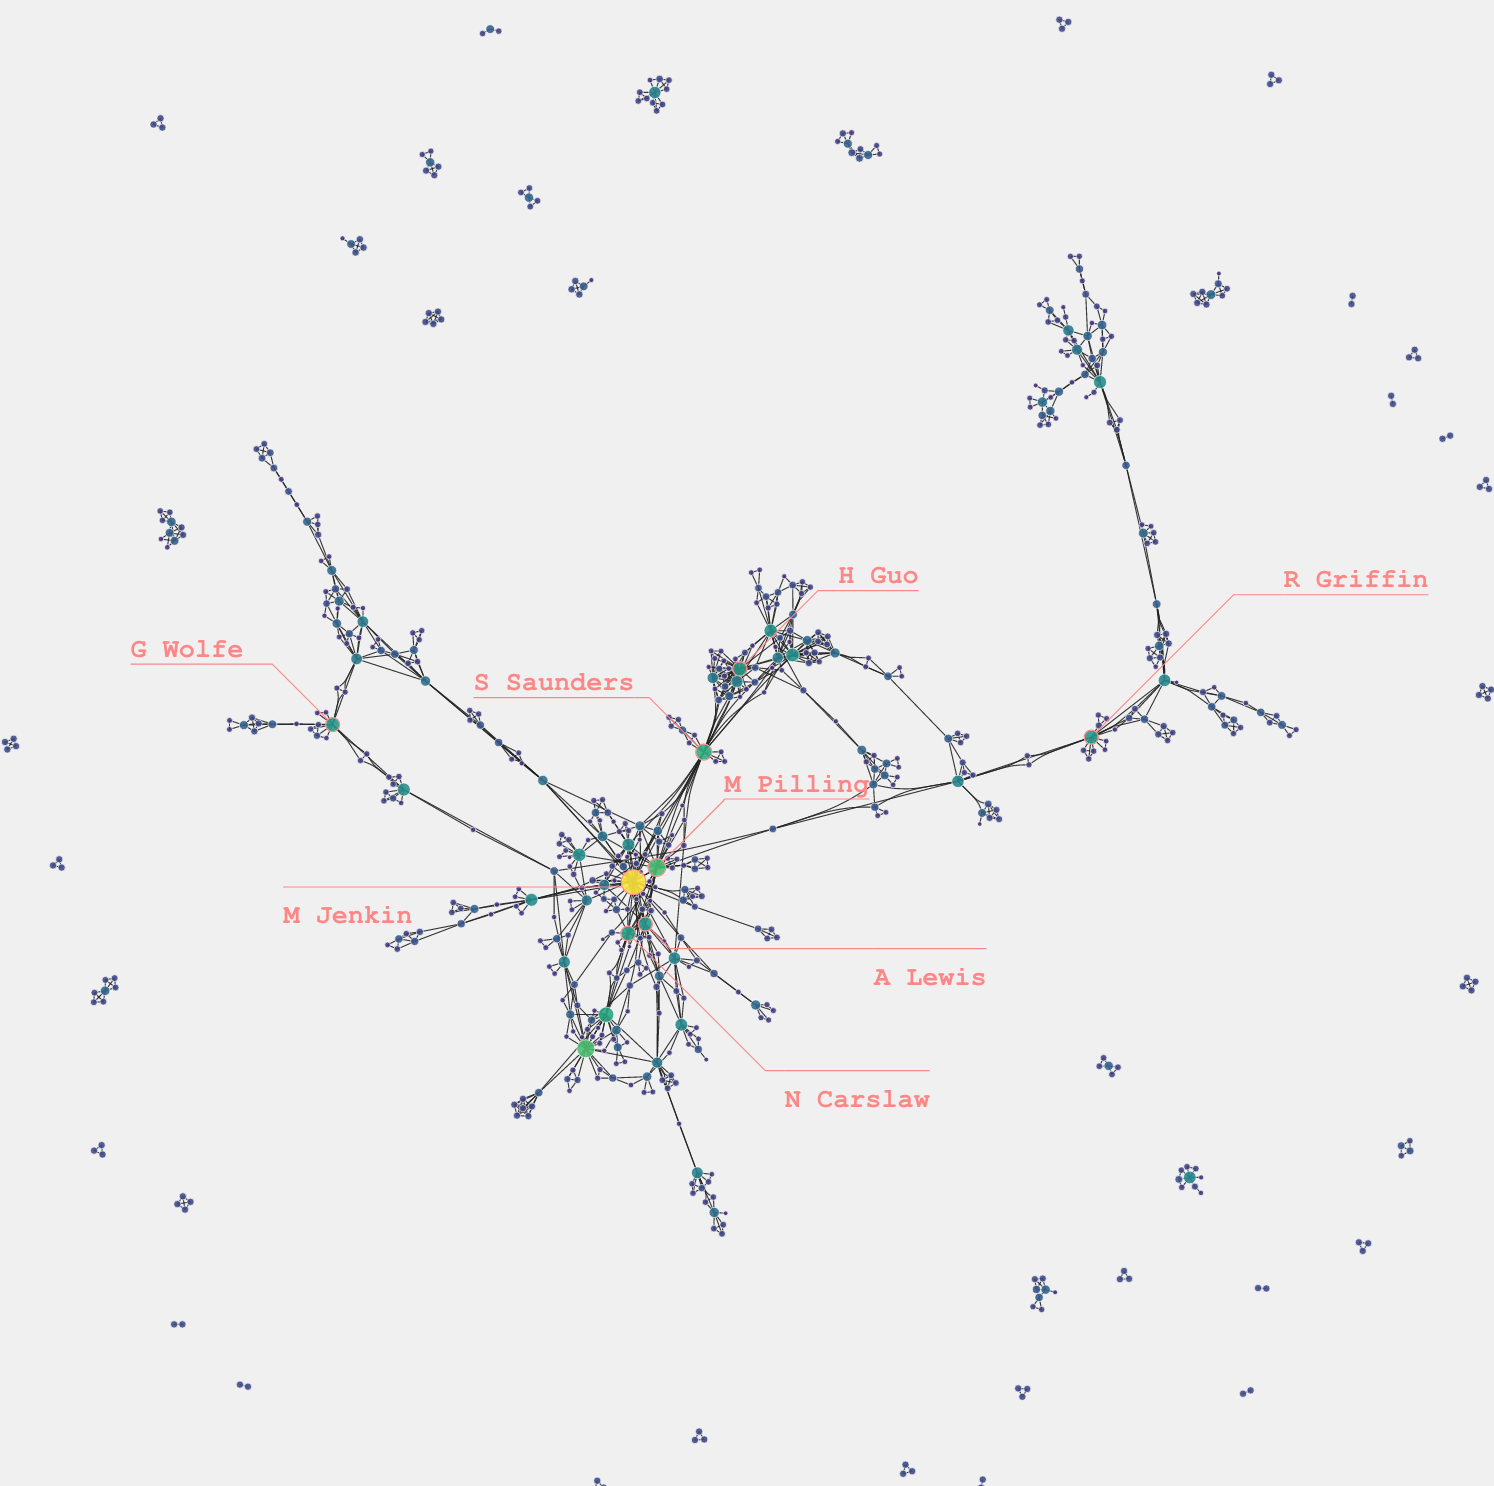
\includegraphics[width=.8\textwidth]{figures_c3/pagerankauthor.png}

        \begin{table}[H] \centering\begin{tabular}{lr}
\toprule
   \hphantom{ } M Jenkin &  0.010435 \\
  \hphantom{ } L Whalley &  0.006589 \\
  \hphantom{ } M Pilling &  0.006488 \\
 \hphantom{ } S Saunders &  0.005591 \\
    \hphantom{ } D Heard &  0.005192 \\
  \hphantom{ } N Carslaw &  0.004833 \\
      \hphantom{ } H Guo &  0.004594 \\
    \hphantom{ } G Wolfe &  0.004523 \\
    \hphantom{ } A Lewis &  0.004508 \\
  \hphantom{ } R Griffin &  0.004500 \\
\bottomrule
\end{tabular}

    \label{tab:pagerank_Author}

    \end{table}

    
                \caption{ \textbf{Page Rank centrality within the co-Author network}. Node size and colour represent the ranking of each node from the page rank algorithm. Larger, lighter coloured nodes are more important.}
        \label{fig:pagerankauth}
\end{figure}


\subsection{Conclusions}
In this section, we have explored the use of centrality metrics to provide us with information on an unweighted co-authorship network of the MCM. Having used these to demonstrate the different roles that may be extracted from a node, we can move on to applying them to a chemical mechanism. In the next section, a global (applying to the network as a whole) set of metrics will be used to determine the network type/structure of the MCM. Once this has been done, graph construction using simulation results (a weighted graph) will be looked into in \autoref{sec:graphconstruction}.
%
%


\section{Classifying The Master Chemical Mechanism Network}\label{sec:globalclass}

Having shown that graph metrics can help the roles of individual nodes within the network, these are now applied to an atmospheric chemical system. Since computational efficiency and resources are often a limiting factor, many applications of the MCM only require a small subset of the entire mechanism. For this reason, it may be of interest to compare these against each other, in an attempt to classify the type of network the MCM chemistry falls under. In this section, we apply graph theory to the entire MCM network to determine its defining characteristics. This is achieved through the analysis of several hundred Monte Carlo selected subsets of the MCM. Each of these is a different combination of the primary emitted VOCs within the MCM v3.3.1.

\subsection{Network Density}\label{sec:netdensity}
Network density is the easiest metric to understand. Visually this can induce complexity and obscure aspects in a graph; mathematically, it can greatly increase the computation time for metrics or algorithms. By definition, we can define network density as a measure of how well connected a node is to every other node. Mathematically it is the ratio of edges against the total number of possible edges for a complete graph\footnote{A complete graph is one where every node is connected to every other node.} of the same size. In chemical terms, we can use this to determine the sparsity of the graph (which has applications on model integrator selection) and give us insights on the chemical structure.  In \autoref{fig:density}, higher numbers of species (nodes) results in an overall decrease in the node-edge ratio - its density. This suggests a modular or hierarchical structure, where new species directly react only with a set number of species, and not the entire mechanism. An explanation for this is that the addition of larger species introduce new branches within the chemistry, which then need to be oxidised before they are small enough to react with the species from a different branch.  Since these branches are somewhat isolated from the rest of the chemistry, they decrease the network density, even though their addition may increase the amount of chemistry that occurs within it.

\begin{figure}[H]
     \centering
         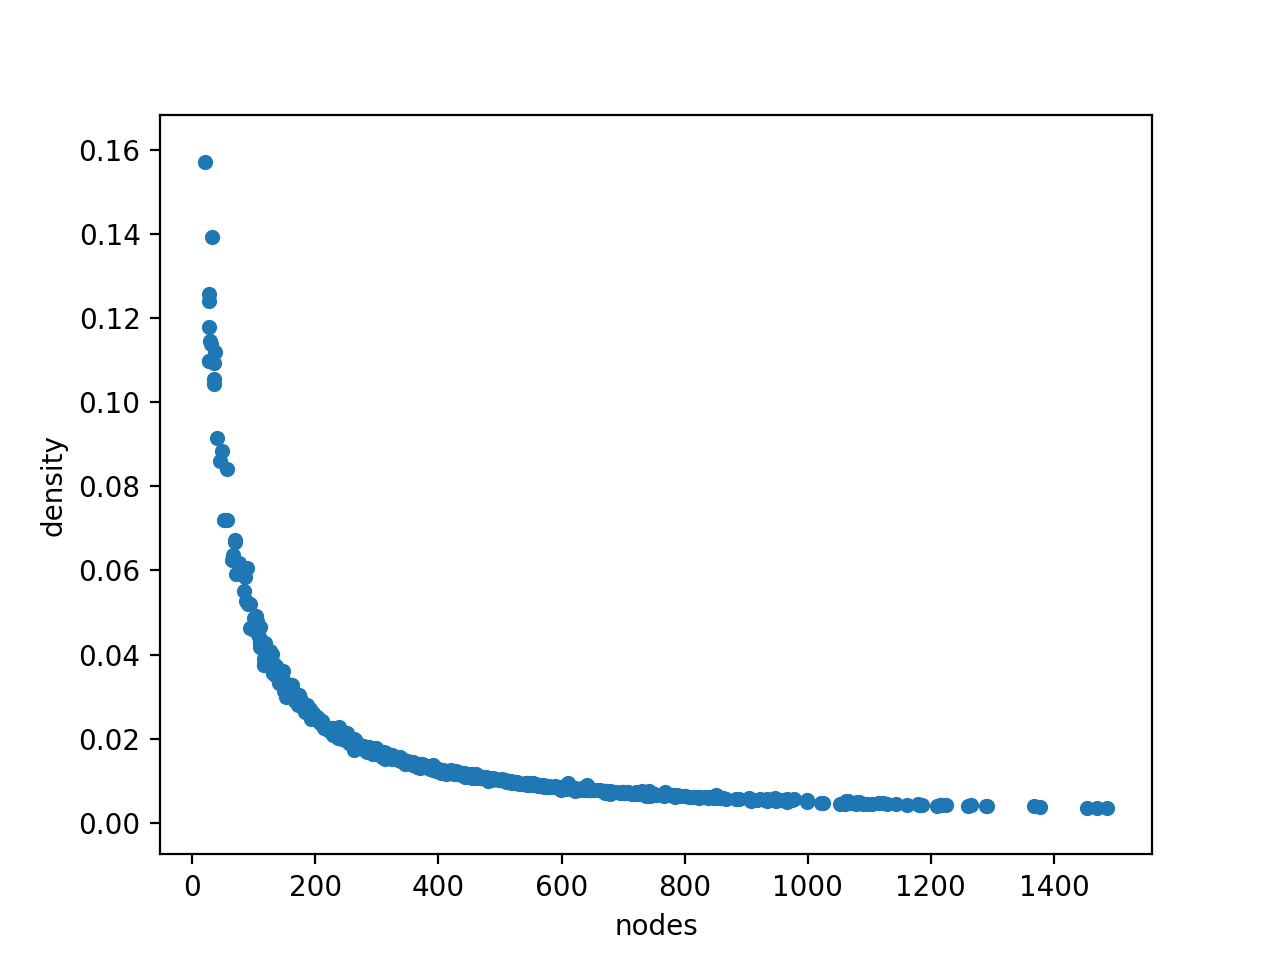
\includegraphics[width=.7\textwidth]{figures_c3/sparcity.png}
        \caption{\textbf{How the MCM graph density scales with number of species.} A figure showing that an increasing number of species within a mechanism subset results in an increased model sparsity (decreasing density).}
        \label{fig:density}
\end{figure}



\subsection{Small World Phenomena}
Within the biological or social sciences the small world phenomenon, colloquially known as `six degrees of separation', is a common occurrence within network structure \citep{smallworld}. Such networks have a large number of localised clusters (cliques) all with a short path length between their elements \citep{sm2}. This makes it easy to reach all parts of a network with only a couple of hops/reactions. In the initial interactive explorations of graph visualisation, it was found that in selecting the reactions of a node, and consequently the reactions of all the nodes which react with them, very quickly a large proportion of the network was highlighted. This suggests that the network may follow the small world phenomena, especially as it is a sparse network, \autoref{sec:netdensity}.

One of the possible methods for establishing the small world-ness of a graph by calculating the omega ($\omega$) coefficient \citep{networkx}:

\begin{equation}
\omega = L_r/L - C/C_l
\end{equation}

Here $C$ is the average clustering coefficient and $L$, the shortest path length of the graph. Comparing these with the average shortest path length, $L_R$, and clustering coefficient $C_l$ (as calculated using an equivalent random and lattice graph) gives the above equation. The output is a result between positive and negative one \{-1,1\}, where a value of 0 suggests the graph exhibits perfect small world-ness.

In assessing the network structure of the MCM, a Monte Carlo (random) approach was taken to extract several hundred subsets from the entire mechanism. For each of these, the omega coefficient was calculated and plotted in \autoref{fig:smw}. Here it is seen that subsets with a small number of species (for example those derived only from methane or ethane) exhibit a more lattice-style (grid) graph, with the majority of the networks showing a more random network structure \autoref{fig:gstructure}. All the results, however, show a prevalence of small-world features over any of the alternative network structures - they are closer to 0 than 1 or -1. This reflects the idea that large species react locally, forming branches (\autoref{ch2}), before oxidising to smaller species with more reactions. This result is also seen within the Reaxys chemical database \citep{rscgraph}.



\begin{figure}[H]
     \centering
         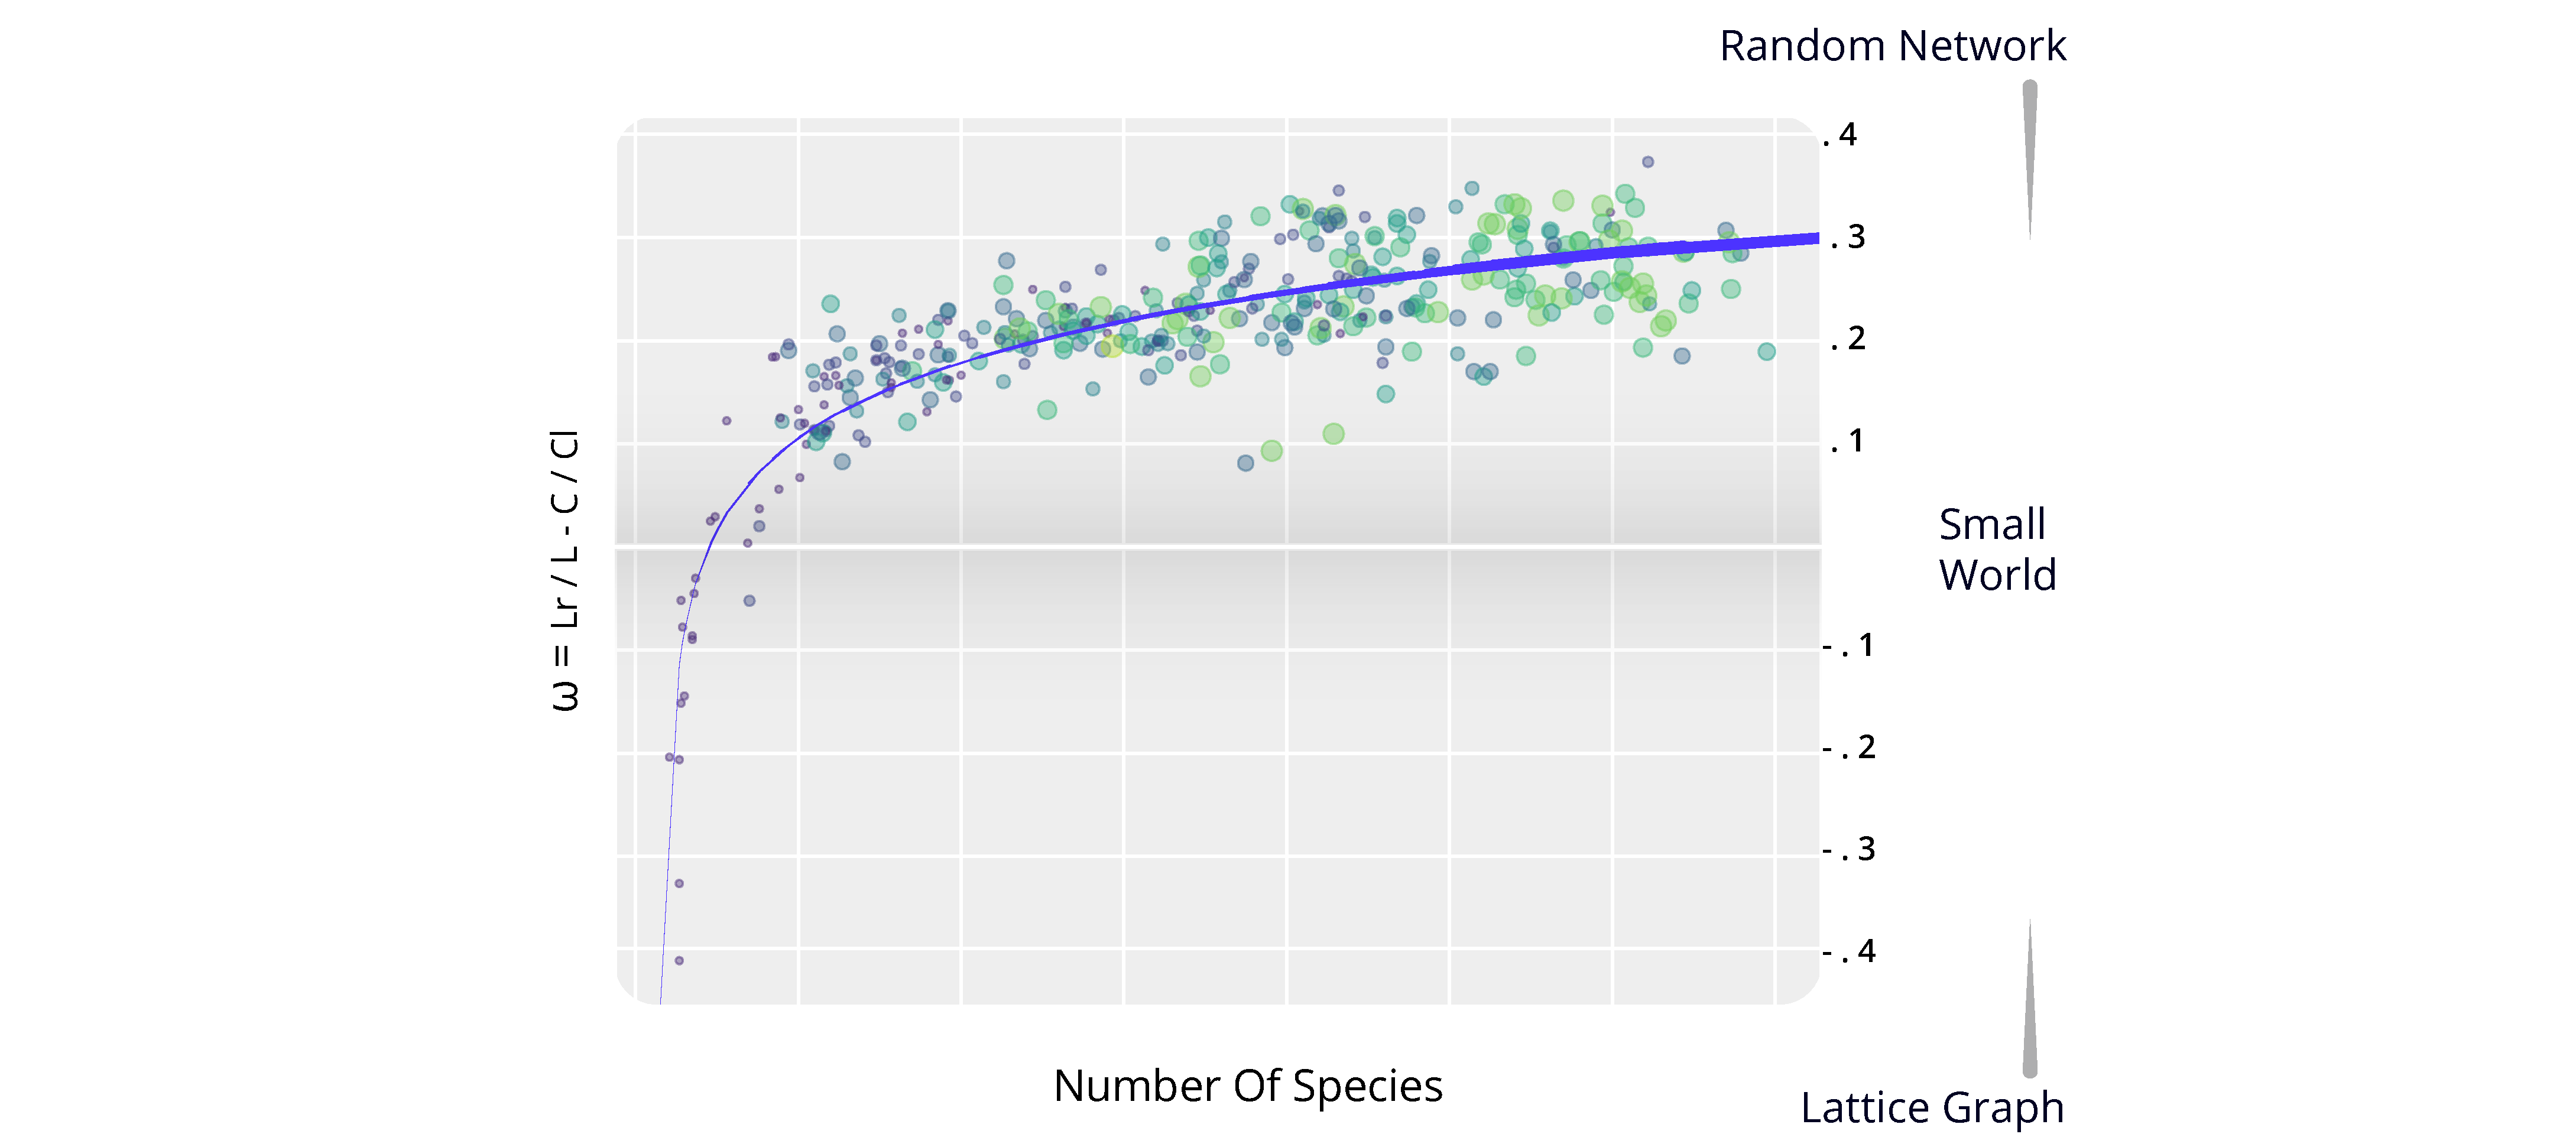
\includegraphics[width=\textwidth]{figures_c3/logpart.pdf}
        \caption{\textbf{A figure showing the small worldness for many Monte-Carlo selected MCM subsets}. The network structure of these is then assessed using the omega coefficient, with [-1,0,1] corresponding to the perfect lattice, small-world and random network structure. Here Node size and colour represents the number of reactions in the mechanism subset and the number of primary VOCs (blue=small, green=large).}
        \label{fig:smw}
\end{figure}



\subsection{Power Law And Scale-Free Graphs}
In real-world applications, it is common to have a hierarchical structure. These are often seen in the increase of citation counts in academic papers \citep{scalefreepapers}, email threads \citep{scalefreeemail} and the world wide web \citep{neoj4}. Unlike random or small-world graphs, scale-free graphs take a hub-and-spoke structure (\autoref{fig:gstructure}), which follows a power-law distribution - that is that scaling probability $p(x) \propto x^{-\alpha}$, where $\alpha$ is a constant and known as the scaling parameter.

\cite{scalefreebad} suggests that scale-free networks are rare, and often misdiagnosed with incorrect tests, or the misinterpretation of power-law features in a network. Similarly, \cite{plexp} suggests that even if the data distribution of a graph is well represented by the power-law distribution, in many cases a logarithmic or exponential distribution may have a better fit.

\begin{figure}[H]
     \centering
         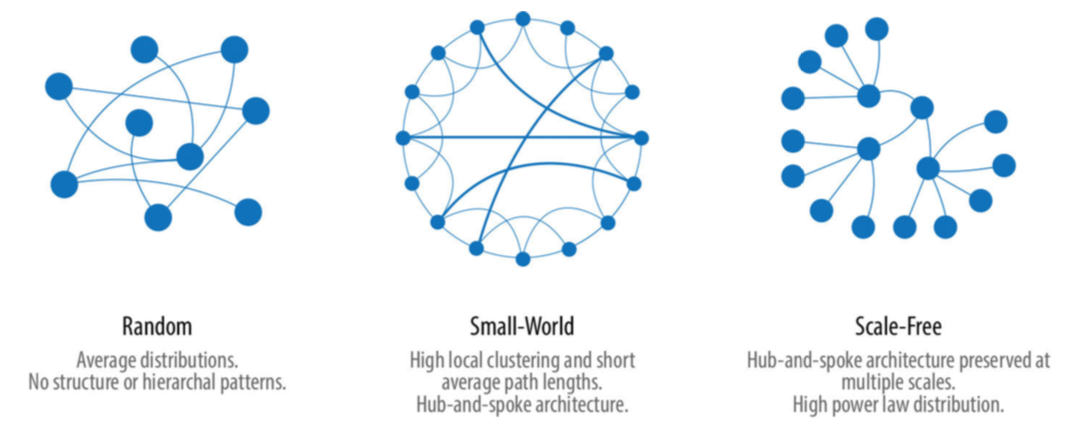
\includegraphics[width=.8\textwidth]{figures_c3/graphstyles.png}
        \caption{\textbf{The different network structures}. A visual depiction of the different graph structures. Source: \cite{neoj4}}
        \label{fig:gstructure}
\end{figure}

To assess the best distribution for describing the Monte Carlo subsets of the MCM, the Kolomogorov-Smirnov statistic \citep{ks} was used to analyse the goodness of fit of the $\omega$ coefficient in \autoref{fig:smw} to a number of distributions. This calculates the maximum distance $D$ between the selected cumelative distribution function $S(x)$ (In our case the Logarithmic, Exponential and Power Law) of the data and the fitted model $P(x)$:

\begin{equation}
D = \smash{\displaystyle\max_{x \ge x_{min}}} |{S(x) - P(x)}|
\end{equation}

Using the MCM subsets from \autoref{fig:smw}, \autoref{fig:ksd} shows that out of the three tested distributions, the MCM is best represented as a power-law distribution (smaller KS distances are better). Although this is not entirely within the chosen 5\% significance, it is highly indicative that some aspects of the network are indeed scale-free.

\begin{figure}[H]
     \centering
         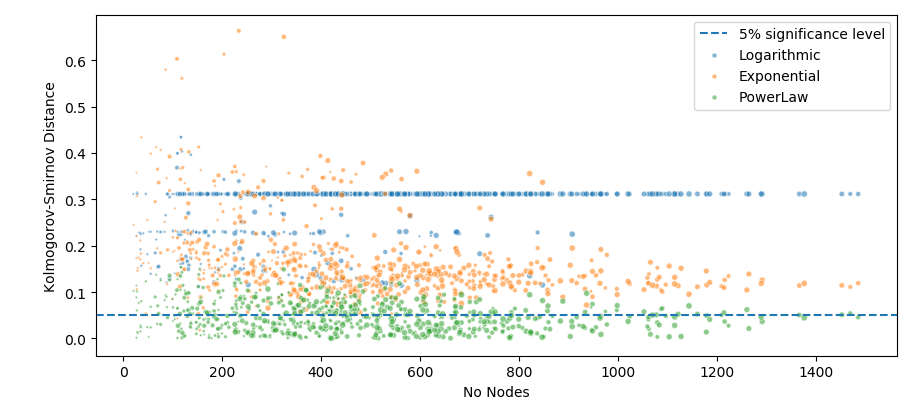
\includegraphics[width=\textwidth]{figures_c3/KSdistance.png}
        \caption{\textbf{Comparing the MCM subsets against a power law, logarithmic and exponential distribution.} The fit for different cumulative probability distributions of nodes in the MCM network is compared to determine the type of network hierarchy the chemistry follows. This is done by comparing the distance of the calculated distribution of data against a perfect one using the Kolmogorov-Smirnov test. The closer the two distributions, the lower the KS distance, and the better the fit. }
        \label{fig:ksd}
\end{figure}

\subsection{Describing The MCM Network}
To conclude, the MCM network exhibits both small world and scale-free (power-law) characteristics. This agrees with previous knowledge about the apparent network structure (\autoref{ch2}). Here large primary emitted hydrocarbons produce branches of a hierarchical nature, as they are progressively broken down into smaller species. Since smaller species are then able to react with a much higher range of species, they then begin to form a tightly connected core, which exhibits many small-world features.

Having classified the MCM network type, the next section will look at how MCM based simulation results can be converted into the graph structure for a more in-depth analysis, \autoref{sec:metriccase}.


\section{Graph Construction Methodology }\label{sec:chem}

Thus far, we have only applied a qualitative analysis of the relationships between species in a mechanism. Although this can educate us about the chemistry within a specific system, often a quantitative value for the rate of reaction between different species is required when undergoing scientific evaluation or policy advice. A chemical mechanism is placed within an atmospheric model, initial concentrations are supplied, and the chemistry is propagated forwards\footnote{Or backwards if the adjoint is used.} in time. Currently, there exist three primary model diagnostics which we may use to analyse the importance or role of a species from a simulation (model) output, concentration time-series, rates of loss and the Jacobian.


\subsubsection{Concentration Time Series}

The simplest of these methods look at the abundance of a  species at a specific point in the atmosphere (its concentration ad a specific time). As time moves forwards, chemicals within the atmosphere undergo a range of reactions which result in the making and breaking of bonds - thus the changing from one species to another.

Using the species concentration as a metric, we can map how it changes over time, and how in changing the initial concentrations of a simulation can produce different results. This can be useful for looking at a range of possible scenarios and evaluating the potential outcome after a pre-determined amount of time. An example would be through the use of policy-based simulations to predict changes in air composition over cities.

Using a simple example from a methane only subset of the MCM (\autoref{fig:concentration}), it is possible to observe the inverse relationship between \ch{NO2} and \ch{NO} using only their concentration profiles. Here nitrogen monoxide reacts with a \ch{Ro2} species to produce an RO and nitrogen dioxide.
This then photolyses back to nitrogen oxide, releasing oxygen which may go on to form ozone (\autoref{sec:o3prod}). The latter part of this reaction is dependant on photons and therefore can only occur during daytime (mostly).

\begin{figure}[H]
     \centering
         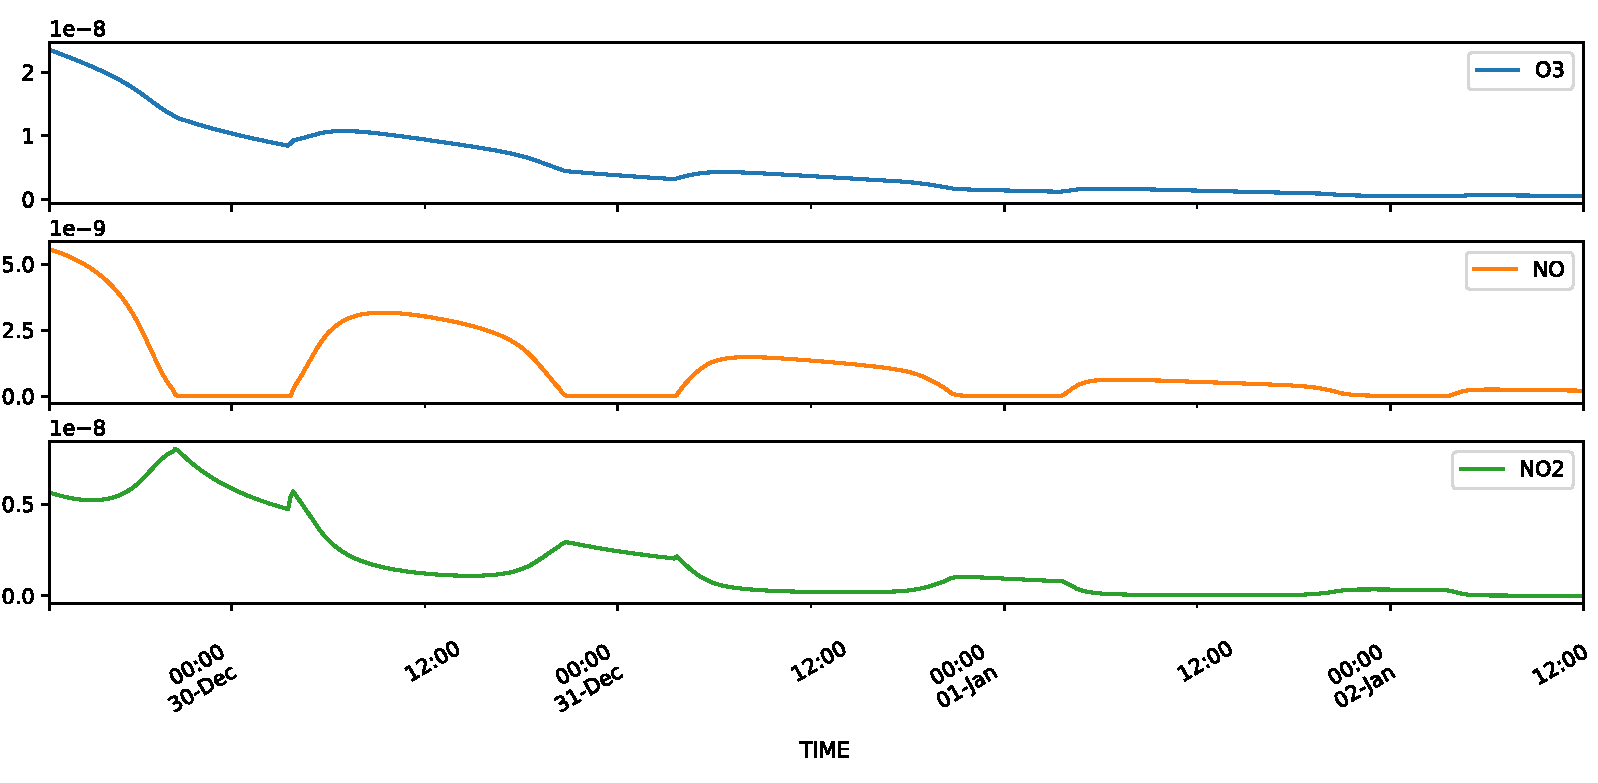
\includegraphics[width=.85\textwidth]{figures/ch2concentration.pdf}\\
         \ce{NO <-->[RO2,O3,HO2][$hv$] NO2}.
        \caption{\textbf{A concentration (mixing ratios) time series from a simple methane-only simulation.} This is the simplest method for identifying changes in species within a model simulation. This multi-plot shows the changes in concentration profiles for all initialised species (NOx:10ppb; \ce{CH4}:20ppb; \ce{O3}:30ppb) following an initial 3 day spin-up to steady state. }
        \label{fig:concentration}
\end{figure}

\subsubsection{Rate Of Production And Loss}\label{sec:ropa}

Analysing the concentration-time profiles allows the comparison of how a series of scenarios or runs change concerning their initial conditions and simulation length. Although these can tell us how, and how much, each species changes over time, it does not rank or quantifies the specific reactions to which this may be attributed. Rate of Production Analysis (ROPA)\footnote{and loss} provides a method for establishing the total contribution from each reaction by calculating the change of concentration (concerning time) for the produced species - the instantaneous reaction flux.

\begin{eqnarray}
  r_1 = A + B \overset{\kappa_1}{\xrightarrow{\hspace*{7mm}}} \eta C & & \text{ Reaction 1}\\[15pt]
  f(C) = \dfrac{\delta C}{\delta t} =  \eta  \kappa_1 [A][B]                     & & \text{ Instantanious Flux }(\Gamma) \label{eqn:ode}
\end{eqnarray}

Here A, B and C are example species; [A],[B] and [C] are species concentrations; $\eta$ and $\omega$ are rate coefficients, and $\kappa$ is the rate of the reaction.

Using a sample simulation representative of the conditions within Beijing (an urban environment), we explore the reactions contributing to the production and loss of \ch{CH3CO3}
(\autoref{fig:ropa_day}) [at noon]. The main reason for this specific example is that it can demonstrate how isolating a specific cause for the change within a species concentration may prove difficult in the context of atmospheric chemistry. Here we have many similarly weighted production and loss reaction, including that of peroxyacetyl nitrate (PAN) and nitrogen dioxide:
\ce{CH3CO3 + NO2 <--> CH3C(O)ONO2} (PAN). The reversible nature, coupled with its near-identical production and loss fluxes produce a tiny net change within our species of interest (\ch{CH3CO3}). Although this may be seen by calculating the cumulative flux between individual species, it is evident that simply looking at the concentrations or highest-ranking reaction fluxes may not be the best method of determining influence. To account for this, we can look at how a change in one species can affect another using the Jacobian method.


\begin{figure}[H]
     \centering
         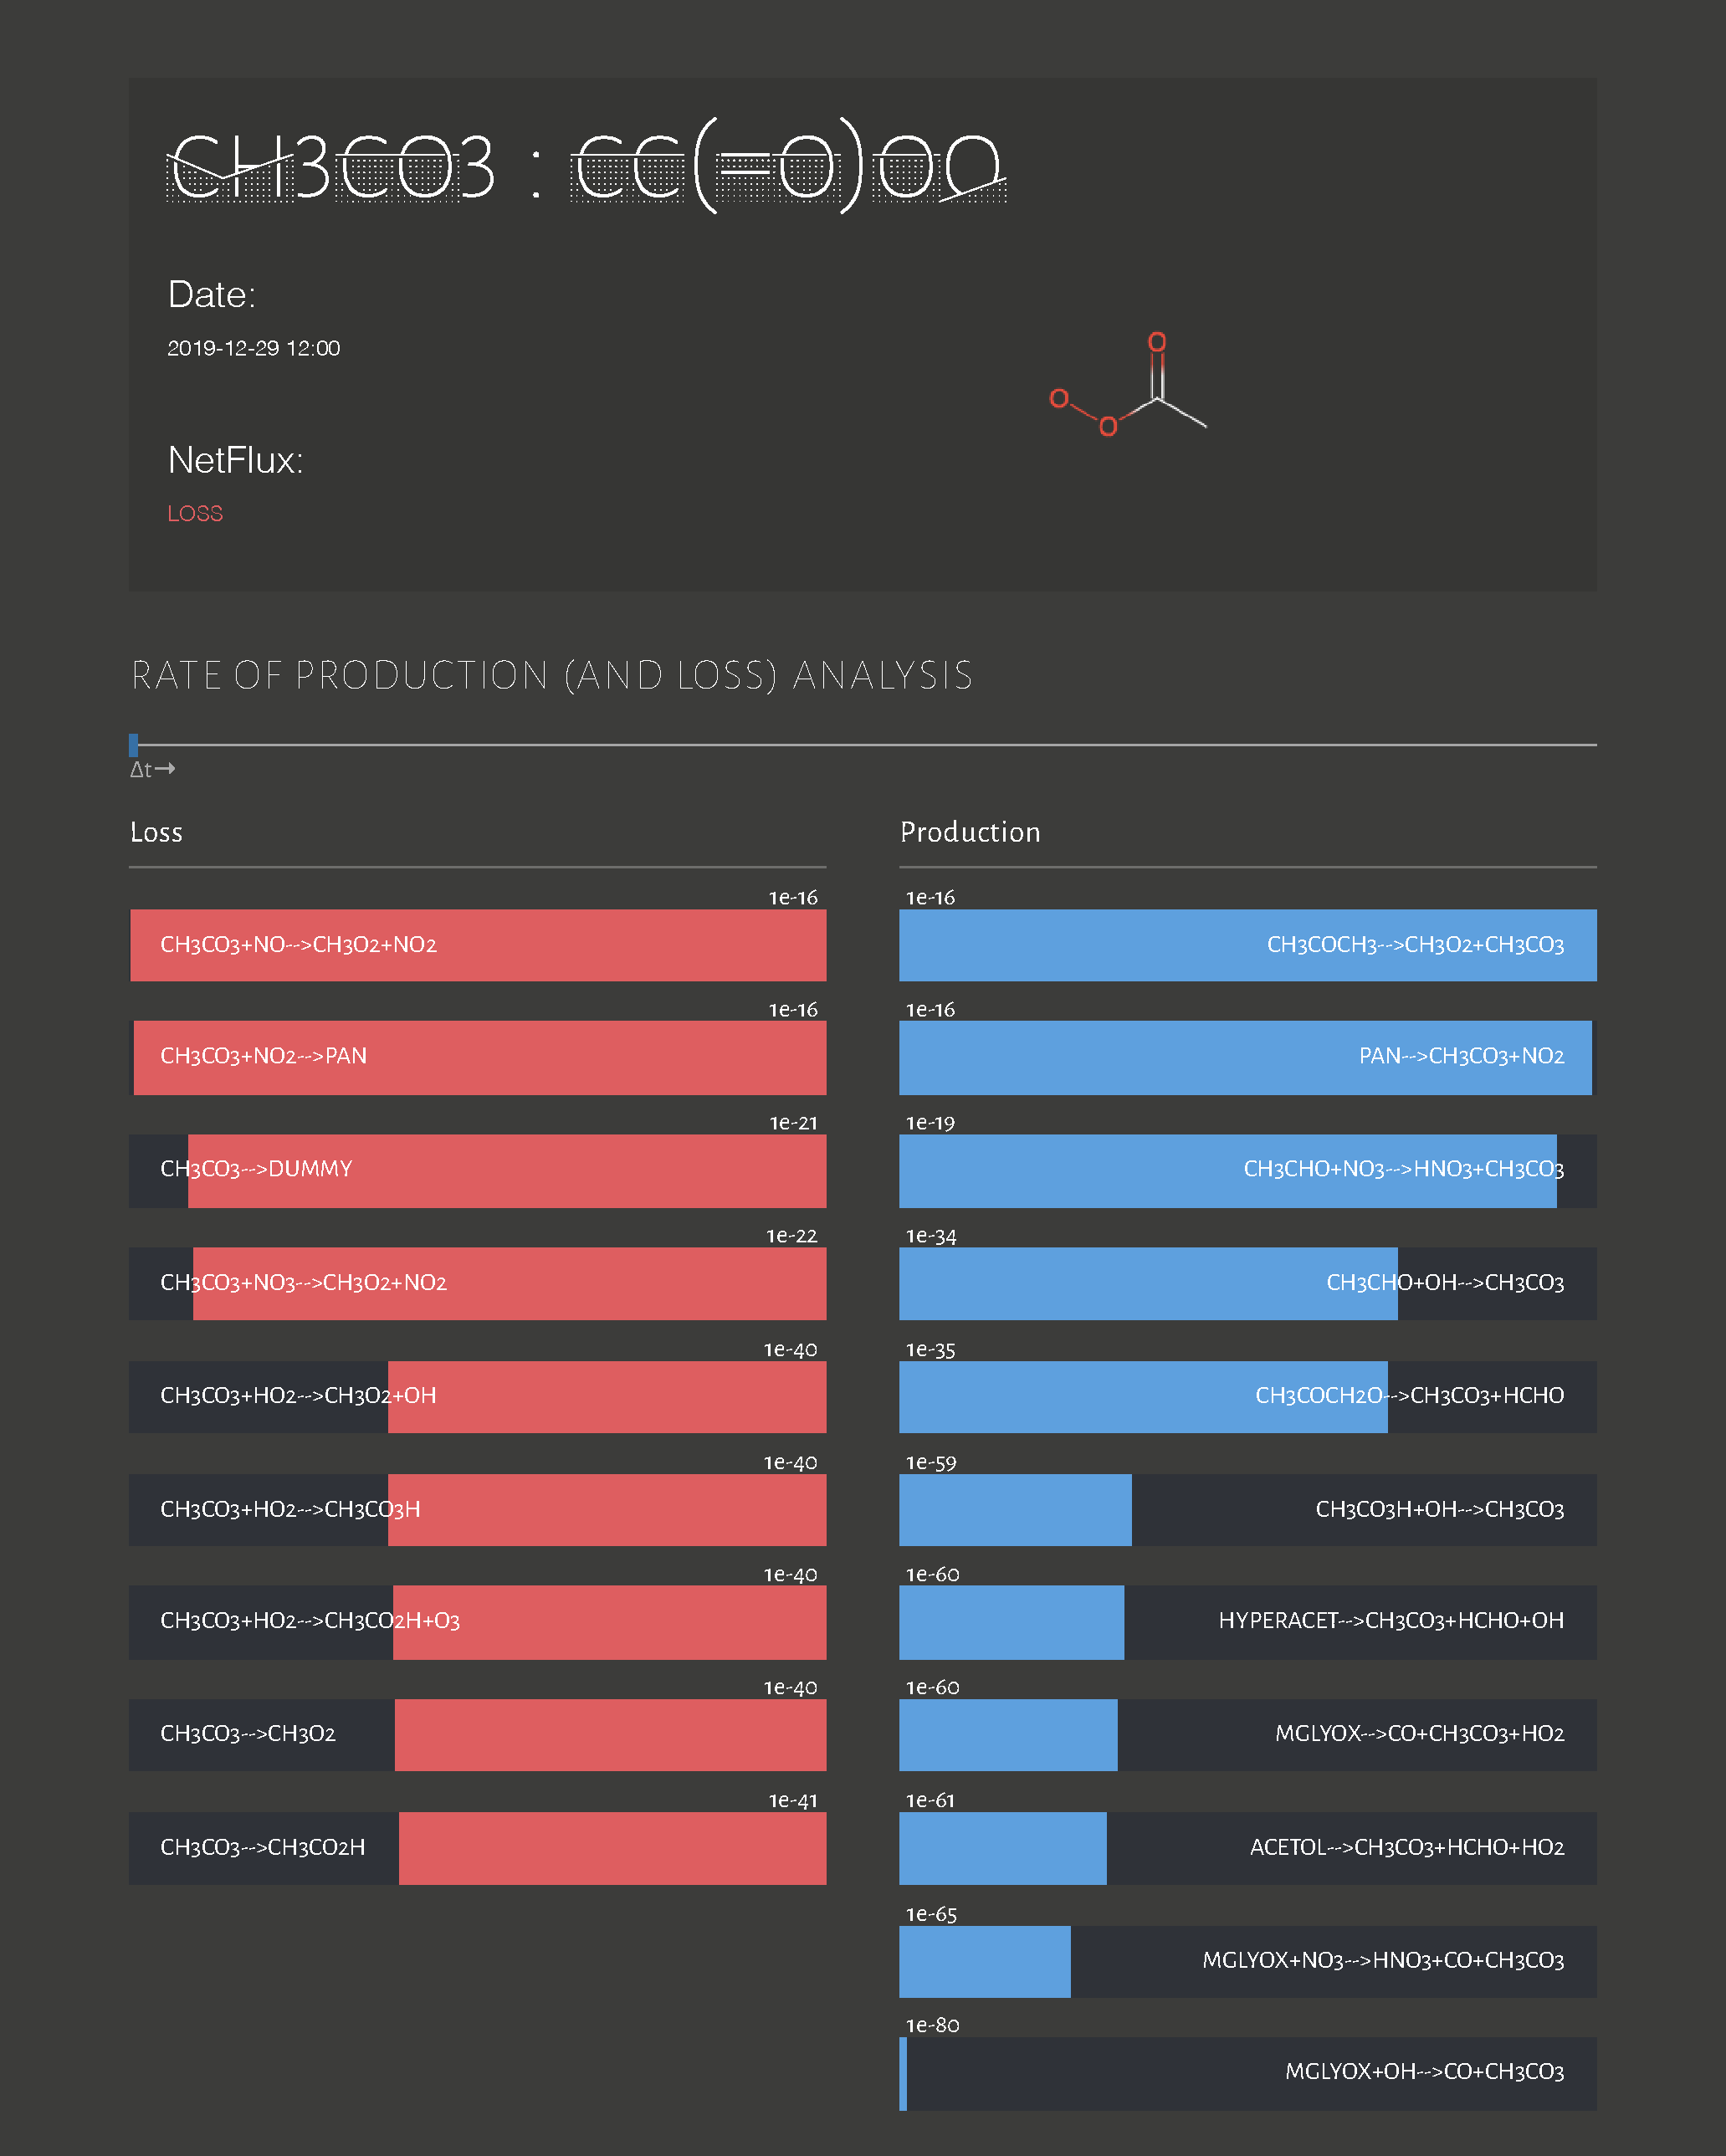
\includegraphics[width=\textwidth]{figures/ROPA_CH3CO3.pdf}
        \caption{\textbf{Rate of production and loss analysis plot for \ch{ch3co3} exhibiting a net loss (daytime).} An example ROPA plot from a simulation representing the chemistry within Beijing. This is used to identify the usefulness and weaknesses of using such a method. DUMMY represents the deposition term for any species. }
        \label{fig:ropa_day}
\end{figure}
\newpage



\subsubsection{The Jacobian}
"The Jacobian [matrix] generalises the notion of gradient to describe the sensitivity to a vector" - \cite{jacob}. That this means is that in taking the partial derivatives of each reaction flux (e.g. from \autoref{eqn:ode}), we can construct a representation of the influence each species has on itself - for example, the influence of species A on C and B on C (\autoref{eqn:A}-\ref{eqn:B}).
\begin{eqnarray}
   \dfrac{\partial \ }{\partial A}\cdot \dfrac{\partial C_{r_1}}{\partial t} = \eta \omega B \kappa_1 & & \Gamma \text{ influence from A }\label{eqn:A}%\\[15pt]
\end{eqnarray}

\begin{eqnarray}
   \dfrac{\partial \ }{\partial B}\cdot \dfrac{\partial C_{r_1}}{\partial t} = \eta \omega A \kappa_1 & &  \Gamma \text{ influence from B }\label{eqn:B}%\\[15pt]
\end{eqnarray}

These partial equations can then be aggregated for all reactions that contain the two species - taking the effect of species B on species C, for example, produces \autoref{eqn:Bsum}. Using these aggregate sums, it is now possible to construct a pairwise relational matrix describing the influence each species has on every other species- \autoref{eqn:jacadj}. This is known as the Jacobian matrix and is to solve the ordinary differential equations which describe the chemistry of the system (and propagate it forwards in time).


\begin{eqnarray}
   \mathbf{J}_{C,B} = \dfrac{\partial f(C) }{\partial B} =
\dfrac{\partial \ }{\partial B} \cdot \left( \dfrac{\partial \Sigma_{r_1}}{\partial t} + \dfrac{\partial \Sigma_{r_2}}{\partial t} + \cdots +\dfrac{\partial \Sigma_{r_n}}{\partial t} \right)
\label{eqn:Bsum}
\end{eqnarray}\\

\begin{eqnarray}
 \mathbf{J}_{i,j} =
 \begin{bmatrix}
   \dfrac{\partial f_1}{\partial v_1} &
     \dfrac{\partial f_1}{\partial v_2} &
     \cdots &
     \dfrac{\partial f_1}{\partial v_n} \\[13pt]
   \dfrac{\partial f_2}{\partial v_1} &
     \dfrac{\partial f_2}{\partial v_2} &
       \cdots &
     \dfrac{\partial f_2}{\partial v_n} \\[13pt]
       \vdots &
     \vdots & \ddots
        &
     \vdots\\[13pt]
   \dfrac{\partial f_n}{\partial v_1} &
     \dfrac{\partial f_n}{\partial v_2} &
       \cdots &
     \dfrac{\partial f_n}{\partial v_n}
 \end{bmatrix}_{i,j=1}^{n,n}
 \label{eqn:jacadj}
\end{eqnarray}



\subsection{Graph Construction Methodology For Simulated Data}\label{sec:graphconstruction}

Having covered the general definition of a Jacobian matrix and how it is constructed, we can now apply it to the context of mechanism analysis and comprehension. The first analogy that needs to be made is that for the flux is the change of a species concentration in time (the first differential with respect to time, $d/dt$). If we consider the change in a species concentration as a `displacement', we can think of the flux as its `velocity'.
Similarly, the Jacobian provides us with a description of how the individual flux of a species changes concerning the concentration (or displacement) or another species (the second-order partial differential). This is analogous to the acceleration of the object or particle we first displaced. In using the Jacobian, we have constructed a relational matrix which outlines the effect a nominal change of a species has on all other species - a concept which is the foundation of the connectivity method (a mechanism reduction technique where all but essential species are removed) \citep{connectivity}.

Since the format of a Jacobian is already in the form of a relational matrix, it can easily be converted to a weighted adjacency matrix, and then directly into the graph format. Since it only considers the aggregated influence between species, much of the work that would otherwise be needed to convert a mechanism into a graph format has already been done. To make use of the Jacobian matrix, several extraction algorithms were written for an updated version of the Dynamically Simple Model of Atmospheric Chemical Complexity (DSMACC) \citep{dsmacc,dsmaccgit}, as discussed in \autoref{ch0}. Here we edit the kinetic pre-processor output, \citep{kpp} to release the values of the Jacobian Matrix and return them at each model timestep for analysis. The process for how this is done is described in \autoref{sec:jacpractical}.



\subsubsection*{ A Note On Using The Flux Instead Of The Jacobian }
\textit{
Depending on the model setup or the users' capabilities, extraction of the Jacobian matrix for each timestep may not be possible. In many cases, the reaction rates and concentration may still be available, allowing for the calculation of reaction fluxes throughout the simulation. If this is the case, the total flux can be calculated using the method described in  \autoref{eqn:ode}. From this, an edge-weighted by a reaction flux can be created from every reactant to each product. This generates a multi-graph (A graph with multiple edges between nodes) which may be simplified by taking the net flux value for all edges between two nodes. \\
However, the potential for human/coding error, additional simplification and a non-explicit definition of the contribution of each species make the use of a Jacobian much more efficient in network generation from a chemical mechanism.
}

\subsection{A Practical Example Using The MCM}\label{sec:jacpractical}

Taking a single equation from the MCM, we may calculate the Jacobian relationships between species and convert them into a graph. A randomly chosen ethane reaction (\autoref{eqn:line}) from a simple mechanism was chosen. In general, the reaction consists of the following two steps:
 \ce{C2H6 + OH ->[\kappa_1] C2H5. + H2O}
and \ce{C2H5. + O2 ->[\kappa_2] CH5O2}.

\begin{equation}
\label{eqn:line}
\text{ \ce{C2H6 + OH ->[\kappa_3] C2H5O2}}
\end{equation}

For simplicity, in this example, this will be the only equation for our mechanism. The resultant Flux \autoref{eqn:exflux} and resultant Jacobian \autoref{eqn:exjac} may be calculated.

\begin{equation}\label{eqn:exflux}
   \Gamma = [\ce{C2H6}][\ce{OH}]\kappa_1 \\[15pt]
\end{equation}

   \begin{eqnarray}
    \mathbf{J}_{i,j} =
 \begin{bmatrix}
   \dfrac{\partial f_{[\ce{C2H6}]}}{\partial t \ \partial {[\ce{C2H6}]}} &
     \dfrac{\partial f_{[\ce{C2H6}]}}{\partial t{[\ce{OH}]}} &
     \dfrac{\partial f_{[\ce{C2H6}]}}{ \partial t{[\ce{C2H5O2}]}} \\[20pt]
   \dfrac{\partial f_{[\ce{OH}]}}{\partial t \ \partial {[\ce{C2H6}]}} &
     \dfrac{\partial f_{[\ce{OH}]}}{\partial t \ \partial {[\ce{OH}]}} &
   \dfrac{\partial f_{[\ce{OH}]}}{\partial t \ \partial {[\ce{C2H5O2}]}} \\[20pt]
   \dfrac{\partial f_{[\ce{C2H5O2}]}}{\partial t \ \partial {[\ce{C2H6}]}} &
     \dfrac{\partial f_{[\ce{C2H5O2}]}}{\partial t \ \partial {[\ce{OH}]}} &
     \dfrac{\partial f_{[\ce{C2H5O2}]}}{\partial t \ \partial {[\ce{C2H5O2}]}}
 \end{bmatrix}_{i,j=1}^{3,3}
 \label{eqn:exjac}
\end{eqnarray}\\


Since not all species react with all other species, (\ce{C2H6} does not react with \ce{C2H5O2}) we can remove reactions that do not exist. To calculate the second differential, we begin by taking the flux of our equation:

\begin{equation}
    \frac{d\ce{C2H5O2}}{dt} = \kappa_3 [\ce{C2H6}][\ce{OH}]
\end{equation}

Using this we can calculate the partial differential equations for OH and \ce{C2H6}:

\begin{eqnarray}
    \frac{\partial ^2 \ \ce{C2H5O2} }{\partial t \ \partial OH} = \kappa_3 [\ce{C2H6}] \\[20pt]
    \frac{\partial ^2 \ \ce{C2H5O2} }{\partial t \ \partial \ce{C2H6}} = \kappa_3 [\ce{OH}]
\end{eqnarray}


This forms a `sparse' Jacobian. Substituting numbers from subset mechanisms containing the methane and ethane precursors, we get \autoref{eqn:exjacsp}.





\begin{eqnarray}
 \mathbf{J}_{i,j} =
\begin{bmatrix}
\dfrac{\partial f_{[\ce{C2H6}]}}{\partial t \ \partial {[\ce{C2H6}]}} &
  - \kappa_3[\ce{C3H6}] &
  \kappa_3[\ce{C3H6}] \\[20pt]
-\kappa_3[\ce{OH}] &
  \dfrac{\partial f_{[\ce{OH}]}}{\partial t \ \partial {[\ce{OH}]}} &
\kappa_3[\ce{OH}] \\[20pt]
\  &
 \  &
  \dfrac{\partial f_{[\ce{C2H5O2}]}}{\partial t \ \partial {[\ce{C2H5O2}]}}
\end{bmatrix}_{i,j=1}^{3,3}
\label{eqn:exjacsppre}
\end{eqnarray}\\



   \begin{eqnarray}
    \mathbf{J}_{i,j} =
 \begin{bmatrix}
   \dfrac{\partial f_{[\ce{C2H6}]}}{\partial t \ \partial {[\ce{C2H6}]}} &
     - 2\times 10^{-7} &
     2\times 10^{-7} \\[20pt]
   -0.1 &
     \dfrac{\partial f_{[\ce{OH}]}}{\partial t \ \partial {[\ce{OH}]}} &
  0.1 \\[20pt]
   \  &
    \  &
     \dfrac{\partial f_{[\ce{C2H5O2}]}}{\partial t \ \partial {[\ce{C2H5O2}]}}
 \end{bmatrix}_{i,j=1}^{3,3}
 \label{eqn:exjacsp}
\end{eqnarray}\\

This creates the Jacobian - a matrix representing the reactions of a mechanism. Here we can calculate the production of a species, by summing of its column (except the diagonal), or its loss (from reacting to produce other species) by summing the row. This relational matrix can be used to generate a weighted graph of the chemistry (\autoref{fig:jacgraph}).

 \begin{figure}[H]
 \begin{center}
 \begin{tikzpicture}[->,>=stealth',shorten >=1pt,auto,node distance=7cm,
                    thick,main node/.style={circle,draw,font=\sffamily\small\bfseries}]

  \node[main node] (1) at (1,4){\ce{OH}};
  \node[main node] (2) at (1,0) {\ce{C2H6}};
  \node[main node] (3) at (7,2) {\ce{C2H5O2}};

  \path[every node/.style={font=\sffamily\small}]
    (1) edge [bend left] node {$2 \times 10^{-7}$} (3)
     (2) edge [bend right] node {$0.1$} (3);

     \path[every node/.style={font=\sffamily\small,color=orange}]
     (1) edge [bend left] node {$-2\times 10^{-7}$} (2)
     (2) edge [bend left] node {$-0.1$} (1);
\end{tikzpicture}

 \end{center}
\caption{ A graphical representation of \autoref{eqn:exjacsp} derrived from the \autoref{eqn:line}}\label{fig:jacgraph}
 \end{figure}

Since any loss edges contain a negative value (orange numbers), it is possible to reverse the direction of the links to produce a positive edge of the same value (\autoref{fig:jacgraphnonneg}).


\begin{figure}[H]
\begin{center}
\begin{tikzpicture}[->,>=stealth',shorten >=1pt,auto,node distance=7cm,
                   thick,main node/.style={circle,draw,font=\sffamily\small\bfseries}]

 \node[main node] (1) at (1,4){\ce{OH}};
 \node[main node] (2) at (1,0) {\ce{C2H6}};
 \node[main node] (3) at (7,2) {\ce{C2H5O2}};

 \path[every node/.style={font=\sffamily\small,color=blue}]
   (1) edge [bend left] node {$2 \times 10^{-7}$} (3)
   (2) edge [bend left ] node {$2\times 10^{-7}$} (1);
   \path[every node/.style={font=\sffamily\small,color=red}]
   (1) edge [bend left] node {$0.1$} (2)
  (2) edge [bend right] node {$0.1$} (3);
\end{tikzpicture}

\end{center}

\caption{ Reversing the directions on negatively weighted edges from \autoref{fig:jacgraph}}\label{fig:jacgraphnonneg}
\end{figure}


After reversing the links, we see that concentration for the reaction between \ch{c2h6} and OH follow the paths:

\begin{eqnarray}
    \ce{OH ->[C2H6][0.1] C2H5O2} \\[20pt]
    \ce{C2H6 ->[OH][2\times10^{-7}] C2H5O2}
\end{eqnarray}



As links in the graph are of the same units, we can simplify the equations by propagating the values of each edge.  This results in a graph with only one link between each product reactant pair (\autoref{fig:jacgraphsim}). It is worth noting that although this method of simplification produces a more intuitive graph, eigenvector metrics such as PageRank automatically transfer the `flow' of information through the system to produce the same result.

\begin{figure}[H]
\begin{center}
\begin{tikzpicture}[->,>=stealth',shorten >=1pt,auto,node distance=7cm,
                   thick,main node/.style={circle,draw,font=\sffamily\small\bfseries}]

 \node[main node] (1) at (1,4){\ce{OH}};
 \node[main node] (2) at (1,0) {\ce{C2H6}};
 \node[main node] (3) at (7,2) {\ce{C2H5O2}};

 \path[every node/.style={font=\sffamily\small,color=blue}]
   (2) edge [bend right] node {$2 \times 10^{-7}$} (3);
   \path[every node/.style={font=\sffamily\small,color=red}]
  (1) edge [bend left] node {$0.1$} (3);
\end{tikzpicture}

\end{center}

\caption{ Simplifying \autoref{fig:jacgraphnonneg}}
\label{fig:jacgraphsim}
\end{figure}


\section{Case Study}\label{sec:metriccase}
In this section, the centrality metrics discussed in \autoref{sec:graphcentrality} are applied to a range of scenarios. These range from polluted urban environments such as London \citep{clfo} and Beijing \cite{aphh}, to marine and terrestrial forest- Cape Verde \citep{capeverde} and Borneo \citep{borneo}. We determine the main drivers for the chemistry and compare the species which are important across each simulation.

\subsection{Establishing Initial Conditions From Observational Data}
Within experimental data assimilation, it is not uncommon to face problems which result in unreliable or missing data. These can range from anything as little as measuring below the instrument sensitivity to powercuts and equipment damage/theft from the local wildlife. This can result in problems when analysing the results and combining them to create a simulation of the chemistry for that environment.

To overcome this, traditionally a combination of data filtration, smoothing and interpolation is required. Although it is possible to fit a diurnal profile, through iterative methods of comparison, and cubic splines, it is more straightforward to implement the method (especially if more data will be added at a later date) is through the use of a Multi-Layer Perceptron Regressor model (MLPRegressor) as provided by the Python package Scikit-Learn, \citep{sklearn}. This is described below.

\subsubsection{The Origin Of Artificial Neural Networks}
The concept of a neural network originated within the field of neuroscience. In biological neurons, signals are sent through the use of electrical impulses using their synapses. When a sufficient number of signals are received within a short timeframe, a neurone will respond, often firing a range of its signals. Using this as a foundation, \cite{pitts} presented a computational model of the biological neuron - the artificial neuron. This has a series of binary inputs and produces a single binary output. This idea was later improved with the invention of the perceptron - a linear classifier which classifies categories by separating them with a straight line. Invented by \cite{perceptron}, this was popularised as a device representative of a modern-day shallow neural network - \citep{perceptronmanual}, \autoref{fig:perceptron}. Unlike the artificial neuron, however, the perceptron can take non-binary (numerical) inputs of an associated weight which allows for the computation of simple linear binary classification. Much like Logistic regression, the perceptron produces a positive or negative classification based on a certain threshold\footnote{It is worth noting that while a Logistic Regression classifier can output a class probability, the use of a hard threshold means that this is not done within the perceptron algorithm \citep{handsonml}}.


\begin{figure}[H]
     \centering
         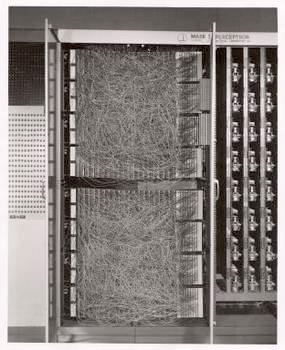
\includegraphics[width=.45\textwidth]{figures_c3/mlpregressor/Mark_I_perceptron.jpg}
        \caption{\textbf{The Mark 1 perceptron} Both software and hardware are different manifestations of a flow chart. The perceptron hardware accomplished what is now done using software. Source: \cite{perceptronimage}}
        \label{fig:perceptron}
\end{figure}

\subsubsection{The Multi-Layer Perceptron}\label{sec:perceptron}
Limitations of the perceptron include the classification of complex patterns such as the XOR problem (where a category appears between two other categories, e.g. {1|0|1} - this cannot be classified by a single linear split). In taking inspiration from nature (\autoref{fig:layercortex}) it is possible to overcome this with the use of multiple layers. This creates a deep ($>2$ two hidden (non-input) layers of perceptrons\footnote{These are sometimes referred to as Linear Threshold Units.}) artificial neural network (ANN)

The multi-layer perceptron (MLP) model now represents a simple feed-forward network, much like a decision tree. However, unlike a decision tree, the MLP ANN can describe the probability a branch is taken using non-linear activation (threshold) functions. These are discussed in detail as part of \autoref{sec:ae}. The weighting thresholds for each neuron are then calculated by backwards propagation of results through the network until a suitably good result is produced.

\begin{quote}
\textit{
\textbf{Example analogy:} Backpropagation can be likened to the iterative calibration of scientific instrumentation. In the field of atmospheric chemistry, laser-induced fluorescence is used to measure species concentrations and reaction rates within the troposphere, \citep{lif1,lif2}. Here the frequency of a laser can be tuned to a resonant frequency of a known target (e.g. \ce{OH}, \ce{NO2} and \ce{SO2}) to produce a response curve.\\
Similarly, a neural network can be `trained' (calibrated).
This is done through the use of a `training dataset' - a set of input-output pairings which represent a random selection of 2/3rds of the total dataset. Next, the neurons within each layer (similar to the potentiometer dials on an instrument) are adjusted in sequence through the layers to match the known result (a standard of known concentration) to the input values provided. This process is repeated until for many iterations, or until a sufficiently `good' prediction is attained for the entire training dataset (early termination). The power of ANNs comes from the ability to adjust neuron thresholds whilst moving both forwards and backwards through the network (Note: predictions of an MLP are still only passed forwards). Finally, model performance is evaluated against the remaining 1/3rd of the total dataset.
}
\end{quote}


\begin{figure}[H]
     \centering
         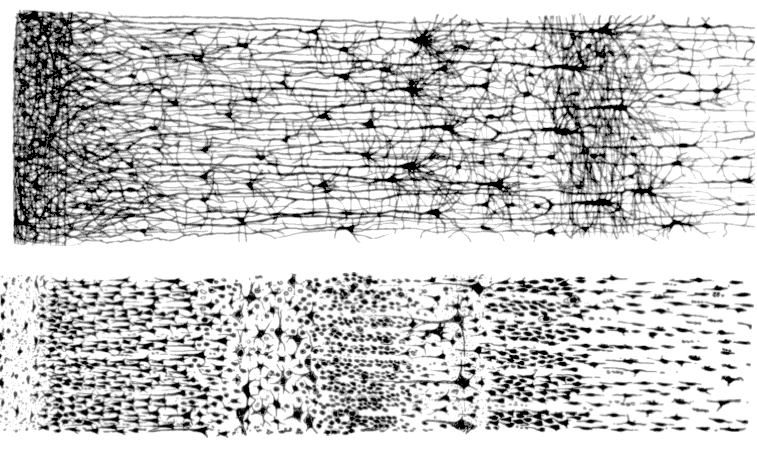
\includegraphics[width=.85\textwidth]{figures_c3/mlpregressor/Cajal_cortex_drawings.png}
        \caption{\textbf{The Human Cortex - A biological neural network.}. A vertical cross section of the human cortex between an adult (top) and 1.5 month old infant (bottom) showing a layer like structure with a change in depth (left to right). Source: \cite{layercortex}}
        \label{fig:layercortex}
\end{figure}

\subsubsection{Applying The Mlpregressor To Observational Data}
In the application of any type of machine aided algorithms, it is important to evaluate the results provided. In this section data collected from Cape Verde (\citep{capeverde}) containing 12 years of observations are shown. A MLPRegressor of 10 hidden layers, and a hyperbolic tan (tanh) activation function is used \autoref{apx:tanh}. Additionally, the limited-memory Broyden–Fletcher–Goldfarb–Shanno (l-BFGS) solver (a quasi-newton method which minimises the inverse of the Hessian matrix\footnote{ The hessian is a square matrix of second-order partial derivatives of a scalar-valued function/field describing the local curvature of a function (of many variables).} to steer through space and obtain a solution) and an adaptive learning rate\footnote{Each time the model improvement fails to decrease the learning loss, the learning rate is reduced by 1/5. This means smaller jumps are made towards the curve peak. } is used.

The input of the regressor is in the form of a month and an hour, to represent each measurement. This allows it to find not only daily trends but also seasonal trends within the data. Once trained, the regressor is then used to predict a diurnal profile for each month based on the observational data provided. For simplicity $\log_{10}$ values of the concentrations obtained have been used. The predicted MLPRegressor line is compared to a transparent scatterplot for all the results. In addition to this, a boxplot showing the Inter Quartile Range (The range between the 25th and 75th percentile), median and mean (green line) plotted alongside to evaluate the predictor output. In this study, we only take the values for the month of June (or closest available depending on the dataset).

In providing the MLPRegressor with both month and hour inputs, the data is not only fitted hourly (a diurnal average) but also across the seasonal/monthly cycles. This accounts for the variation between years and datasets. Since $\log_{10}$ values of the concentrations are used, species such as ozone (\autoref{fig:mlpo3}) which for the Cape Verde dataset (clean air) do not change more than one order of magnitude, the effects of neighbouring months, which shift the diurnal away from the mean (the green line on the boxplot), can be seen. However, since this is overall a small change, and the diurnals lie within the interquartile range, they still provide an adequate approximation. NO (\autoref{fig:mlpno}) on the other hand, has a concentration change of several orders of magnitude. Here a distinct daytime peak is seen and is centred around a seasonally consistent mean value of the data. Here the multi-magnitude change in concentration also provides a striking silhouette of the data to which we may compare the fitted line.
Finally the plots of \ce{NO2} and iso-Pentane (\autoref{fig:mlpno2}-\ref{fig:mlpisopentane}) vary both in diurnal magnitude and seasonally. Within these plots, changes in the data in the January and December months produce deceptively misleading results. Here although the diurnals are not symmetric, they fit well within the median, mean and interquartile range values, as well as the general data silhouette behind them. This suggests that it is a property of the data that we are fitting, and not that the regressor is producing incorrect results. It is however noted that for a more accurate seasonal prediction, periodic boundary conditions should be employed in the training dataset, where an additional two months are added before January and after December. As only a single value estimate from the summer region will be taken, this does not affect the result accuracy.

\begin{figure}[H]
     \centering
         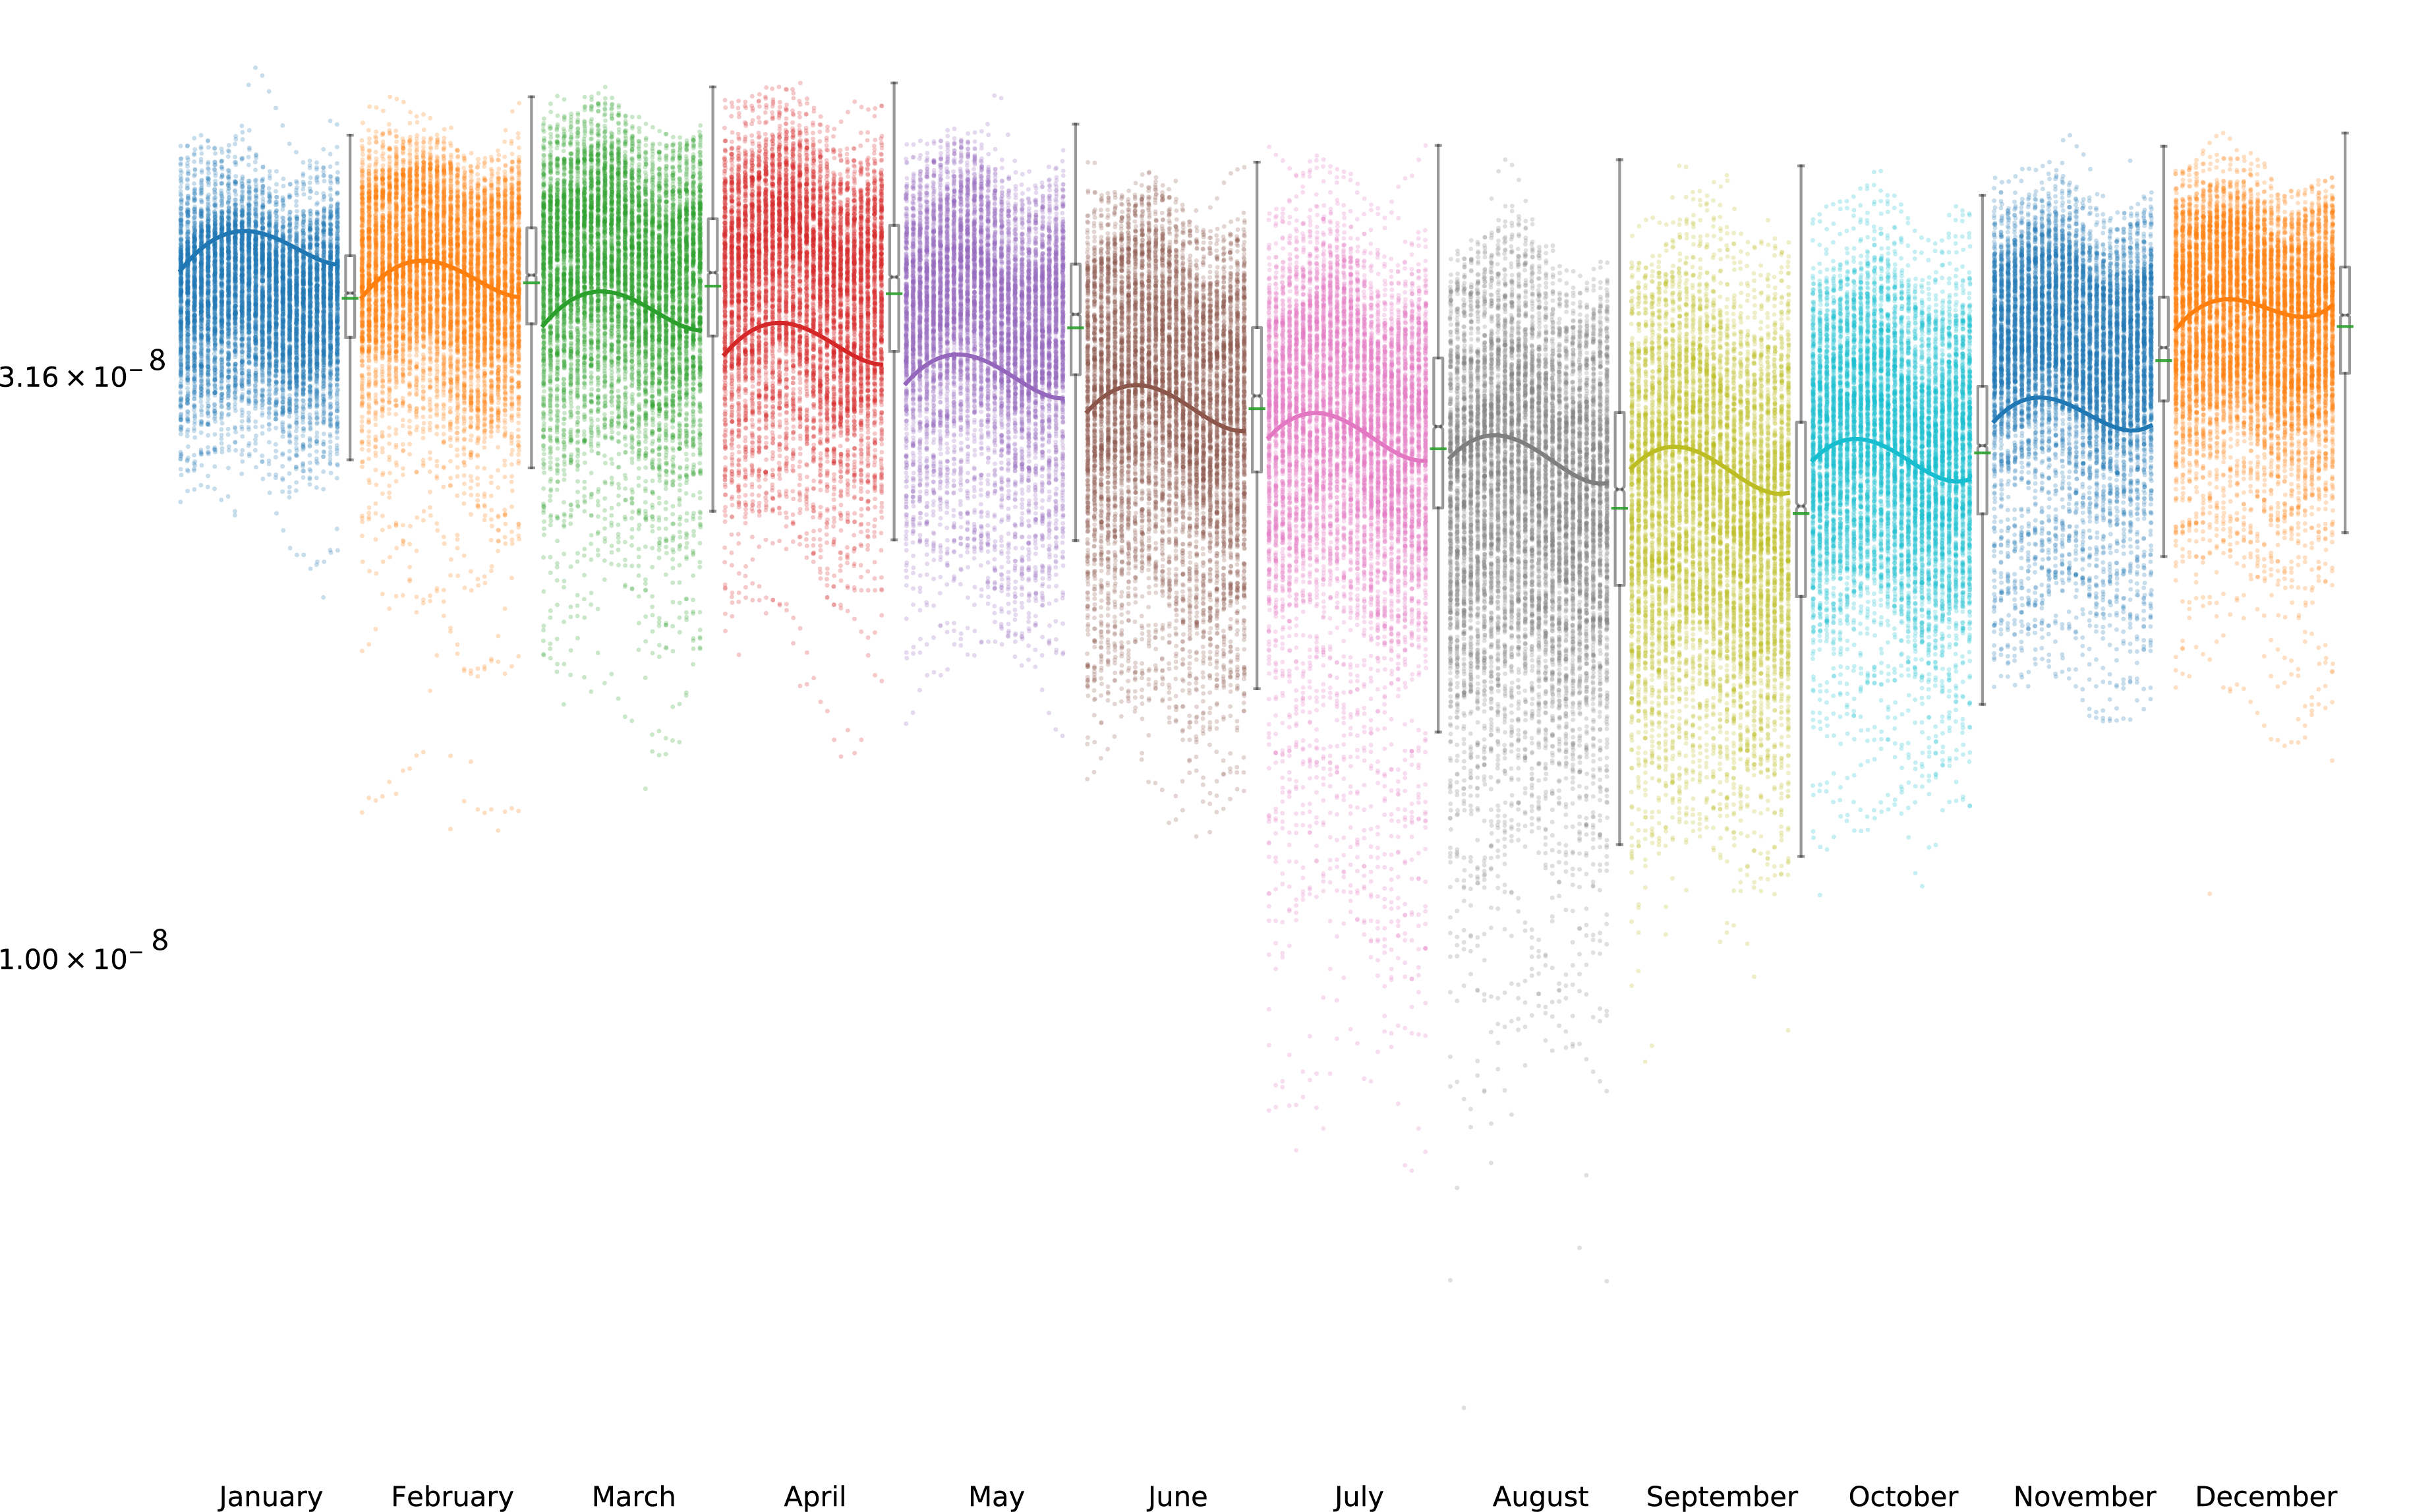
\includegraphics[width=.90\textheight,angle =90,trim={0 0 0 0}]{figures_c3/mlpregressor/CVNOX_CapeVerde/O3.png}
        \caption{\textbf{Cape Verde MLP predicted and observational data of Ozone (mixing ratio).} Each segment represents data from a different month. Within each month segment exists 24 hour segments to create a diurnal. Observational concentrations are plotted in the form of a translucent scatterplot and summarised using the boxplot on the right of the month segment. MLP predicted results are shown using the solid lines. Concentration in mixing ratio.}
        \label{fig:mlpo3}
\end{figure}

\begin{figure}[H]
     \centering
         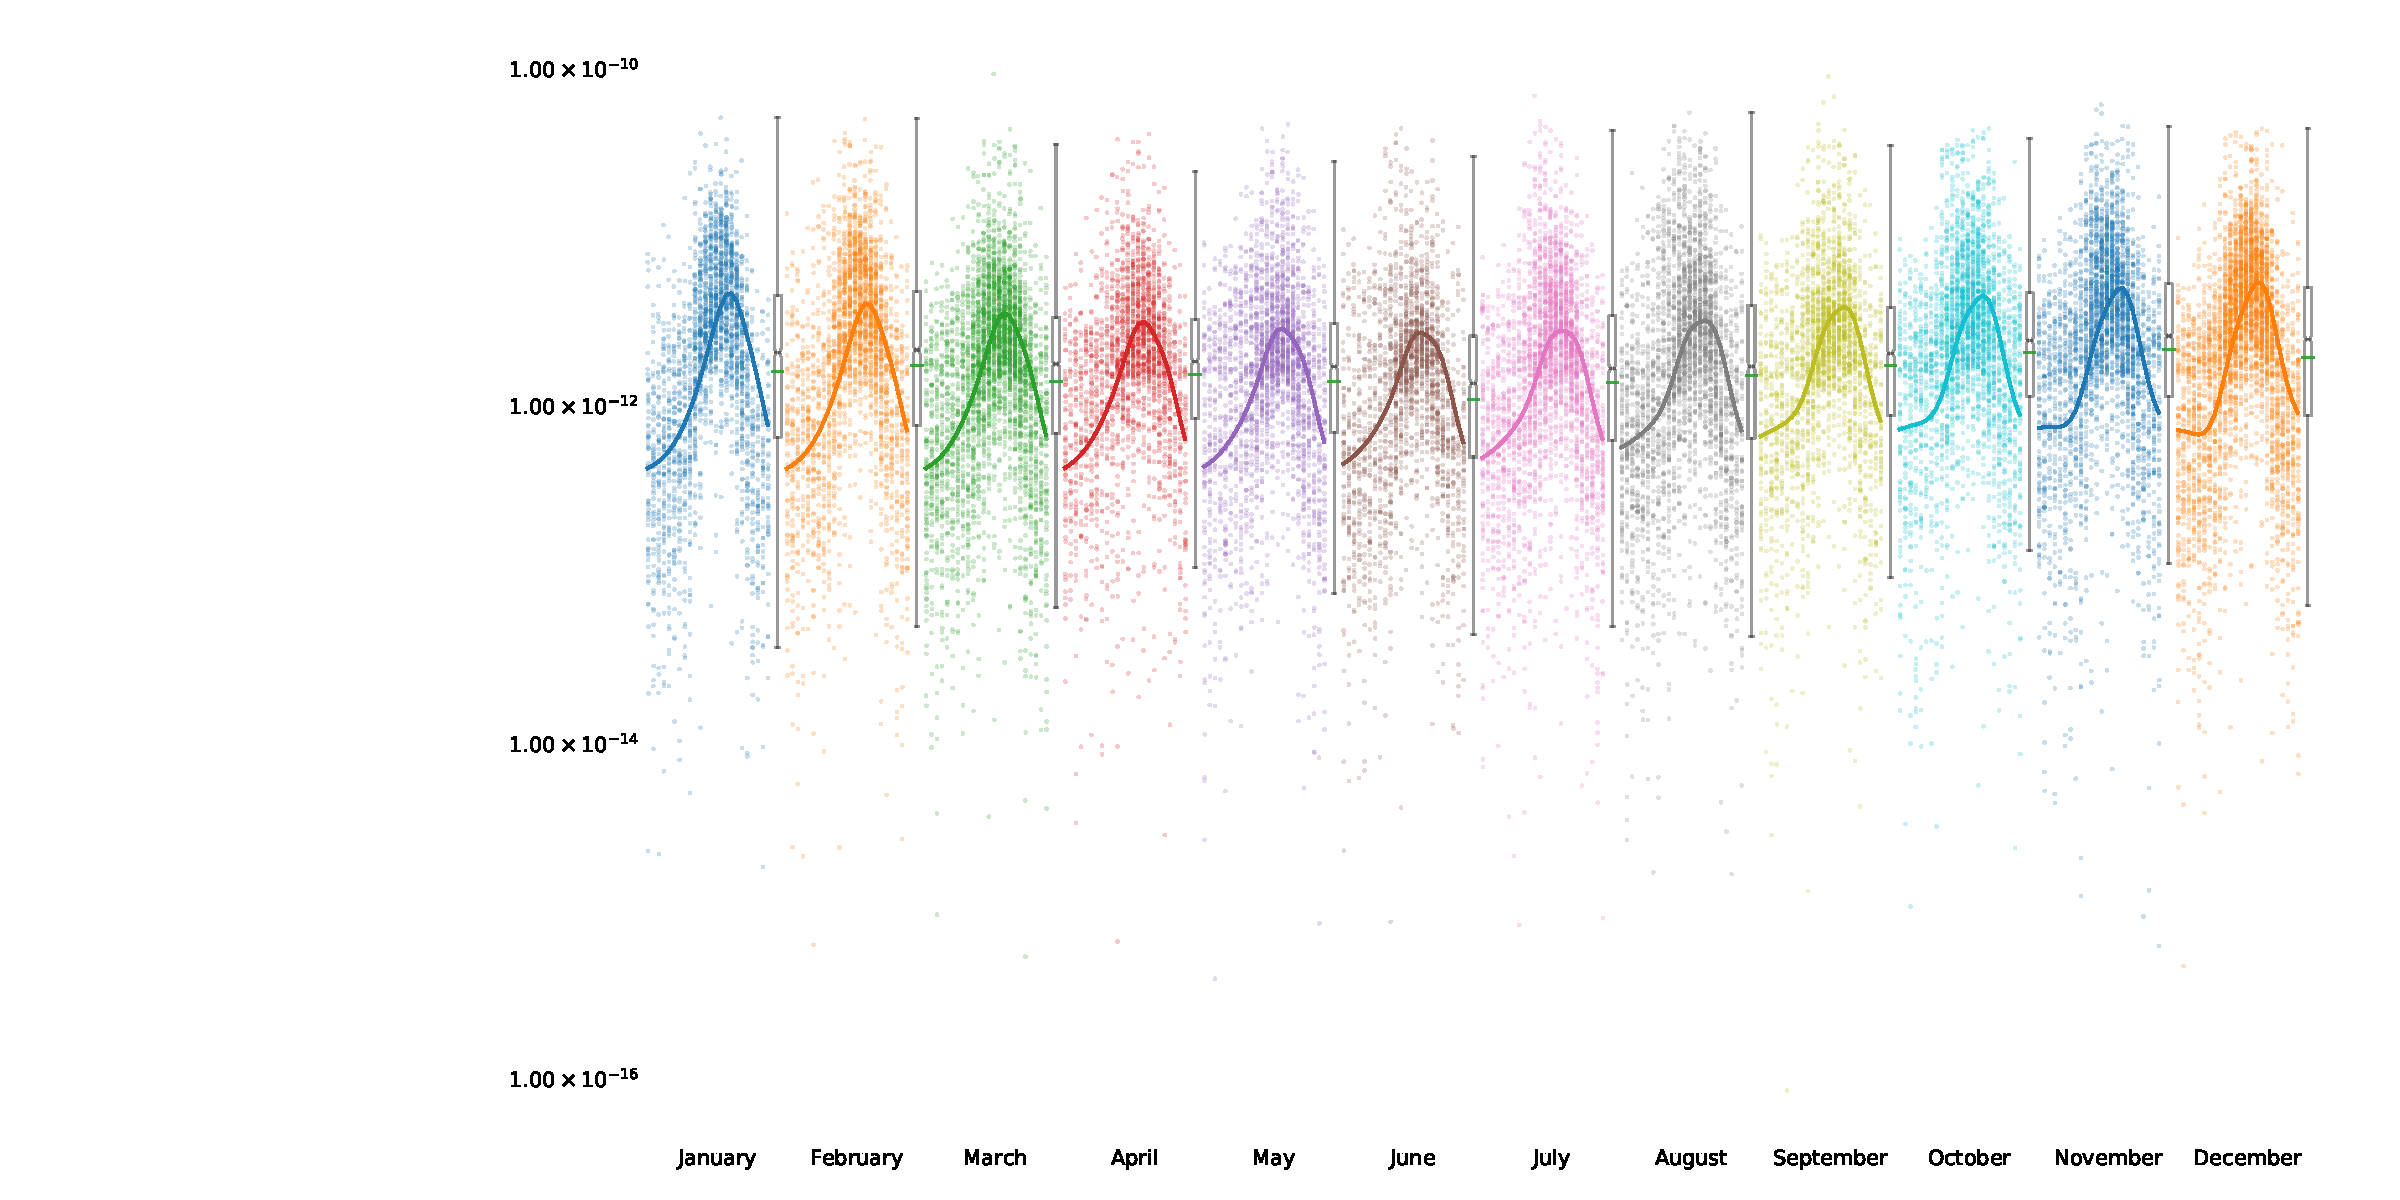
\includegraphics[width=.90\textheight,angle =90,trim={8cm 0 0 0}]{figures_c3/mlpregressor/CVNOX_CapeVerde/NO.pdf}
        \caption{\textbf{Cape Verde MLP predicted and observational data of NO (mixing ratio).} Each segment represents data from a different month. Within each month segment exists 24 hour segments to create a diurnal. Observational concentrations are plotted in the form of a translucent scatterplot and summarised using the boxplot on the right of the month segment. MLP predicted results are shown using the solid lines. Concentration in mixing ratio.}
        \label{fig:mlpno}
\end{figure}

\begin{figure}[H]
     \centering
         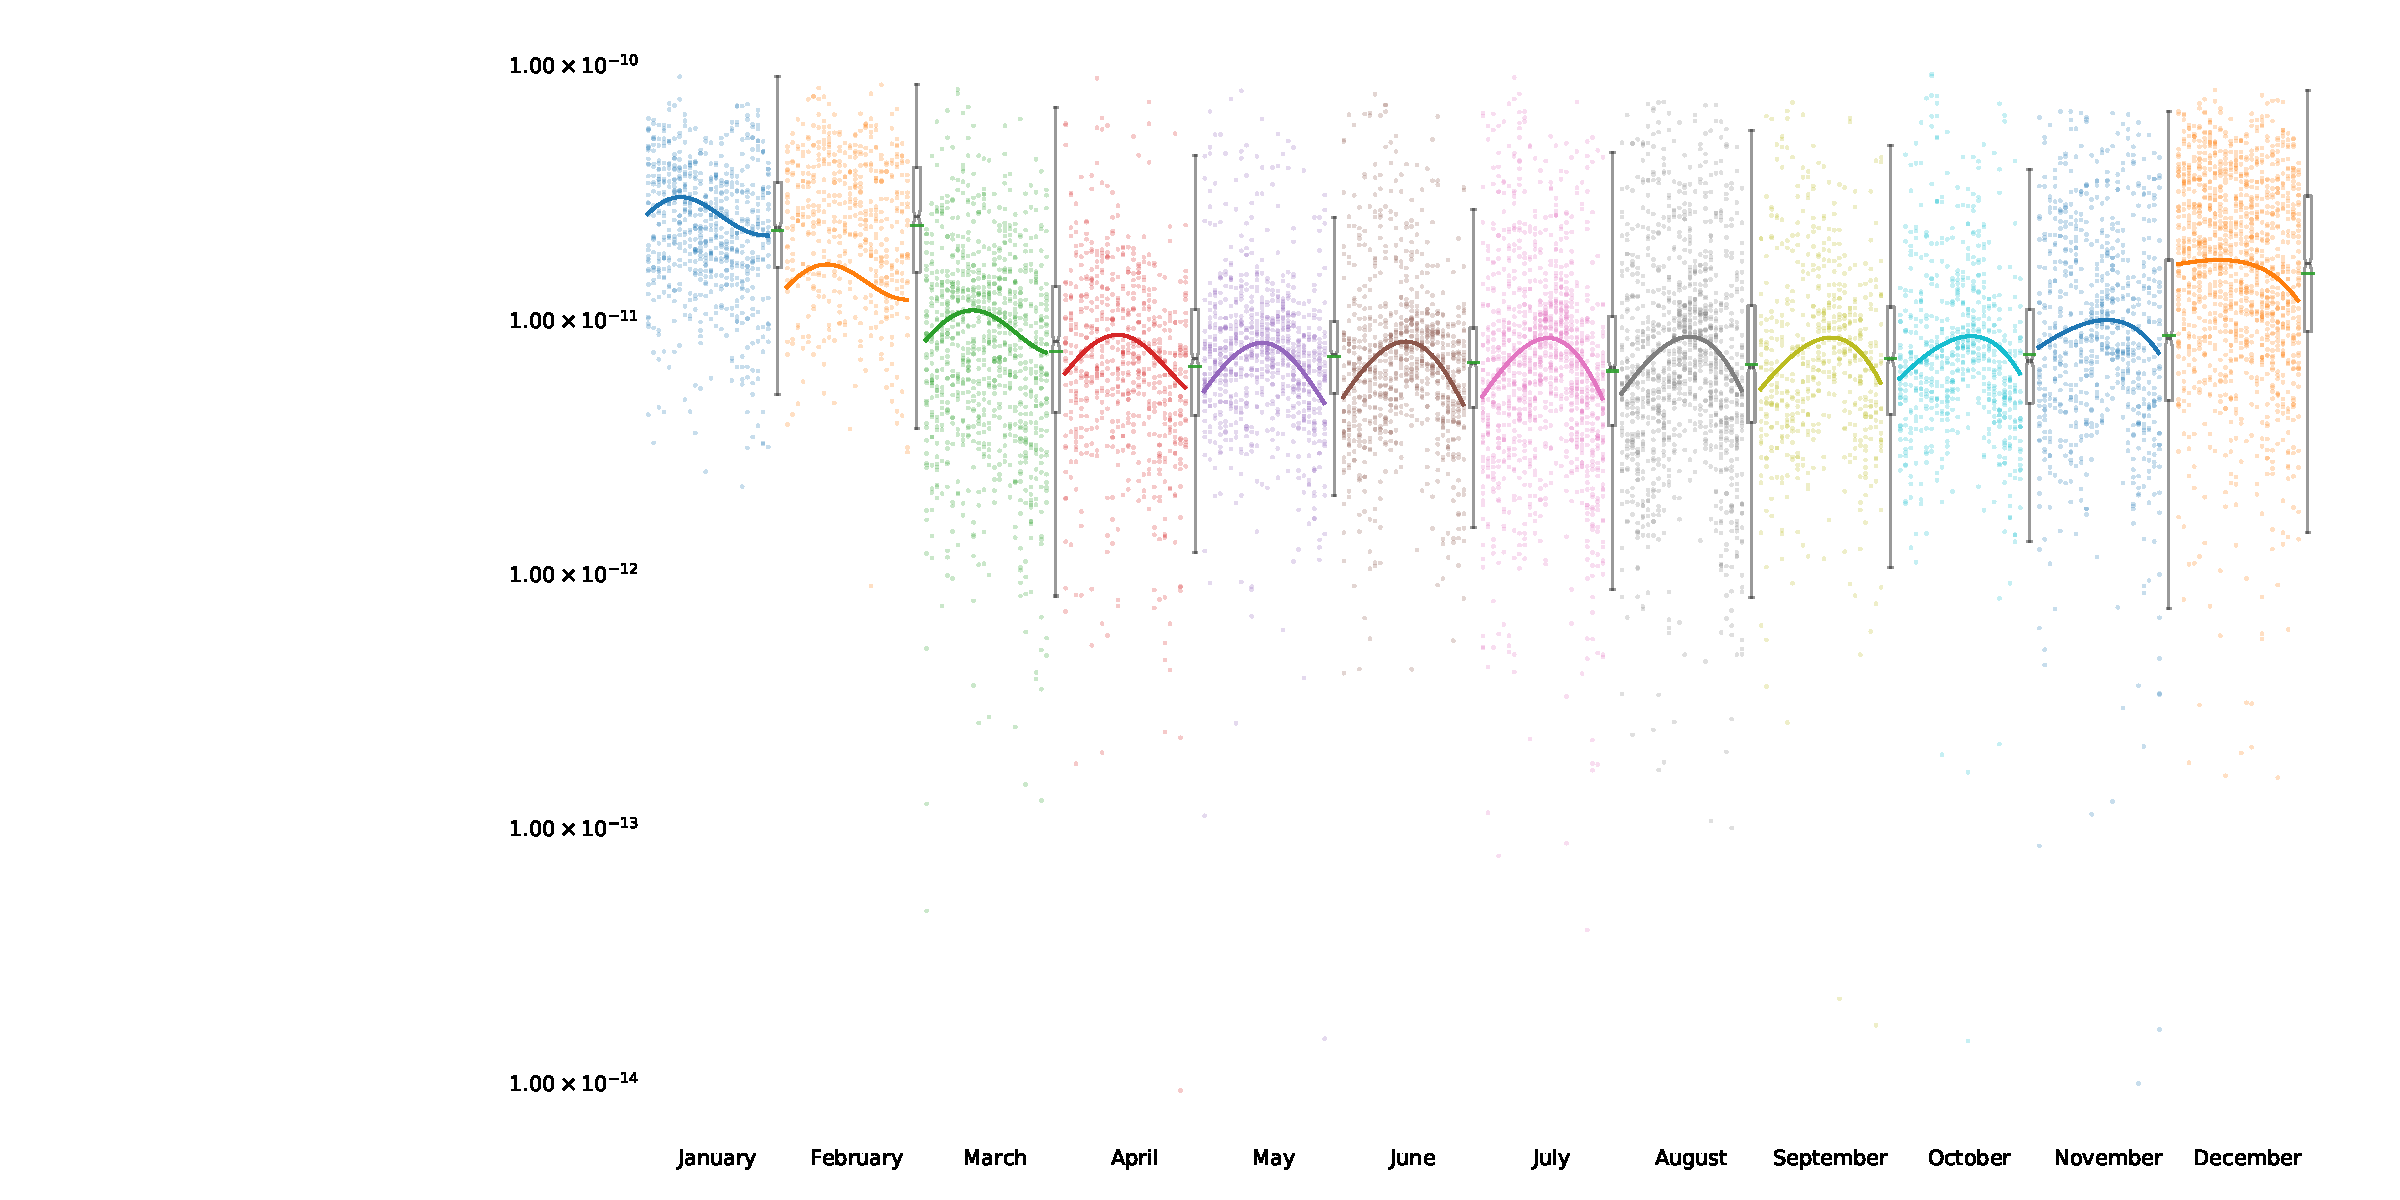
\includegraphics[width=.90\textheight,angle =90,trim={8cm 0 0 0}]{figures_c3/mlpregressor/CVNOX_CapeVerde/NO2.pdf}
        \caption{\textbf{Cape Verde MLP predicted and observational data of \ch{no2} (mixing ratio).} Each segment represents data from a different month. Within each month segment exists 24 hour segments to create a diurnal. Observational concentrations are plotted in the form of a translucent scatterplot and summarised using the boxplot on the right of the month segment. MLP predicted results are shown using the solid lines. Concentration in mixing ratio.}
        \label{fig:mlpno2}
\end{figure}

\begin{figure}[H]
     \centering
         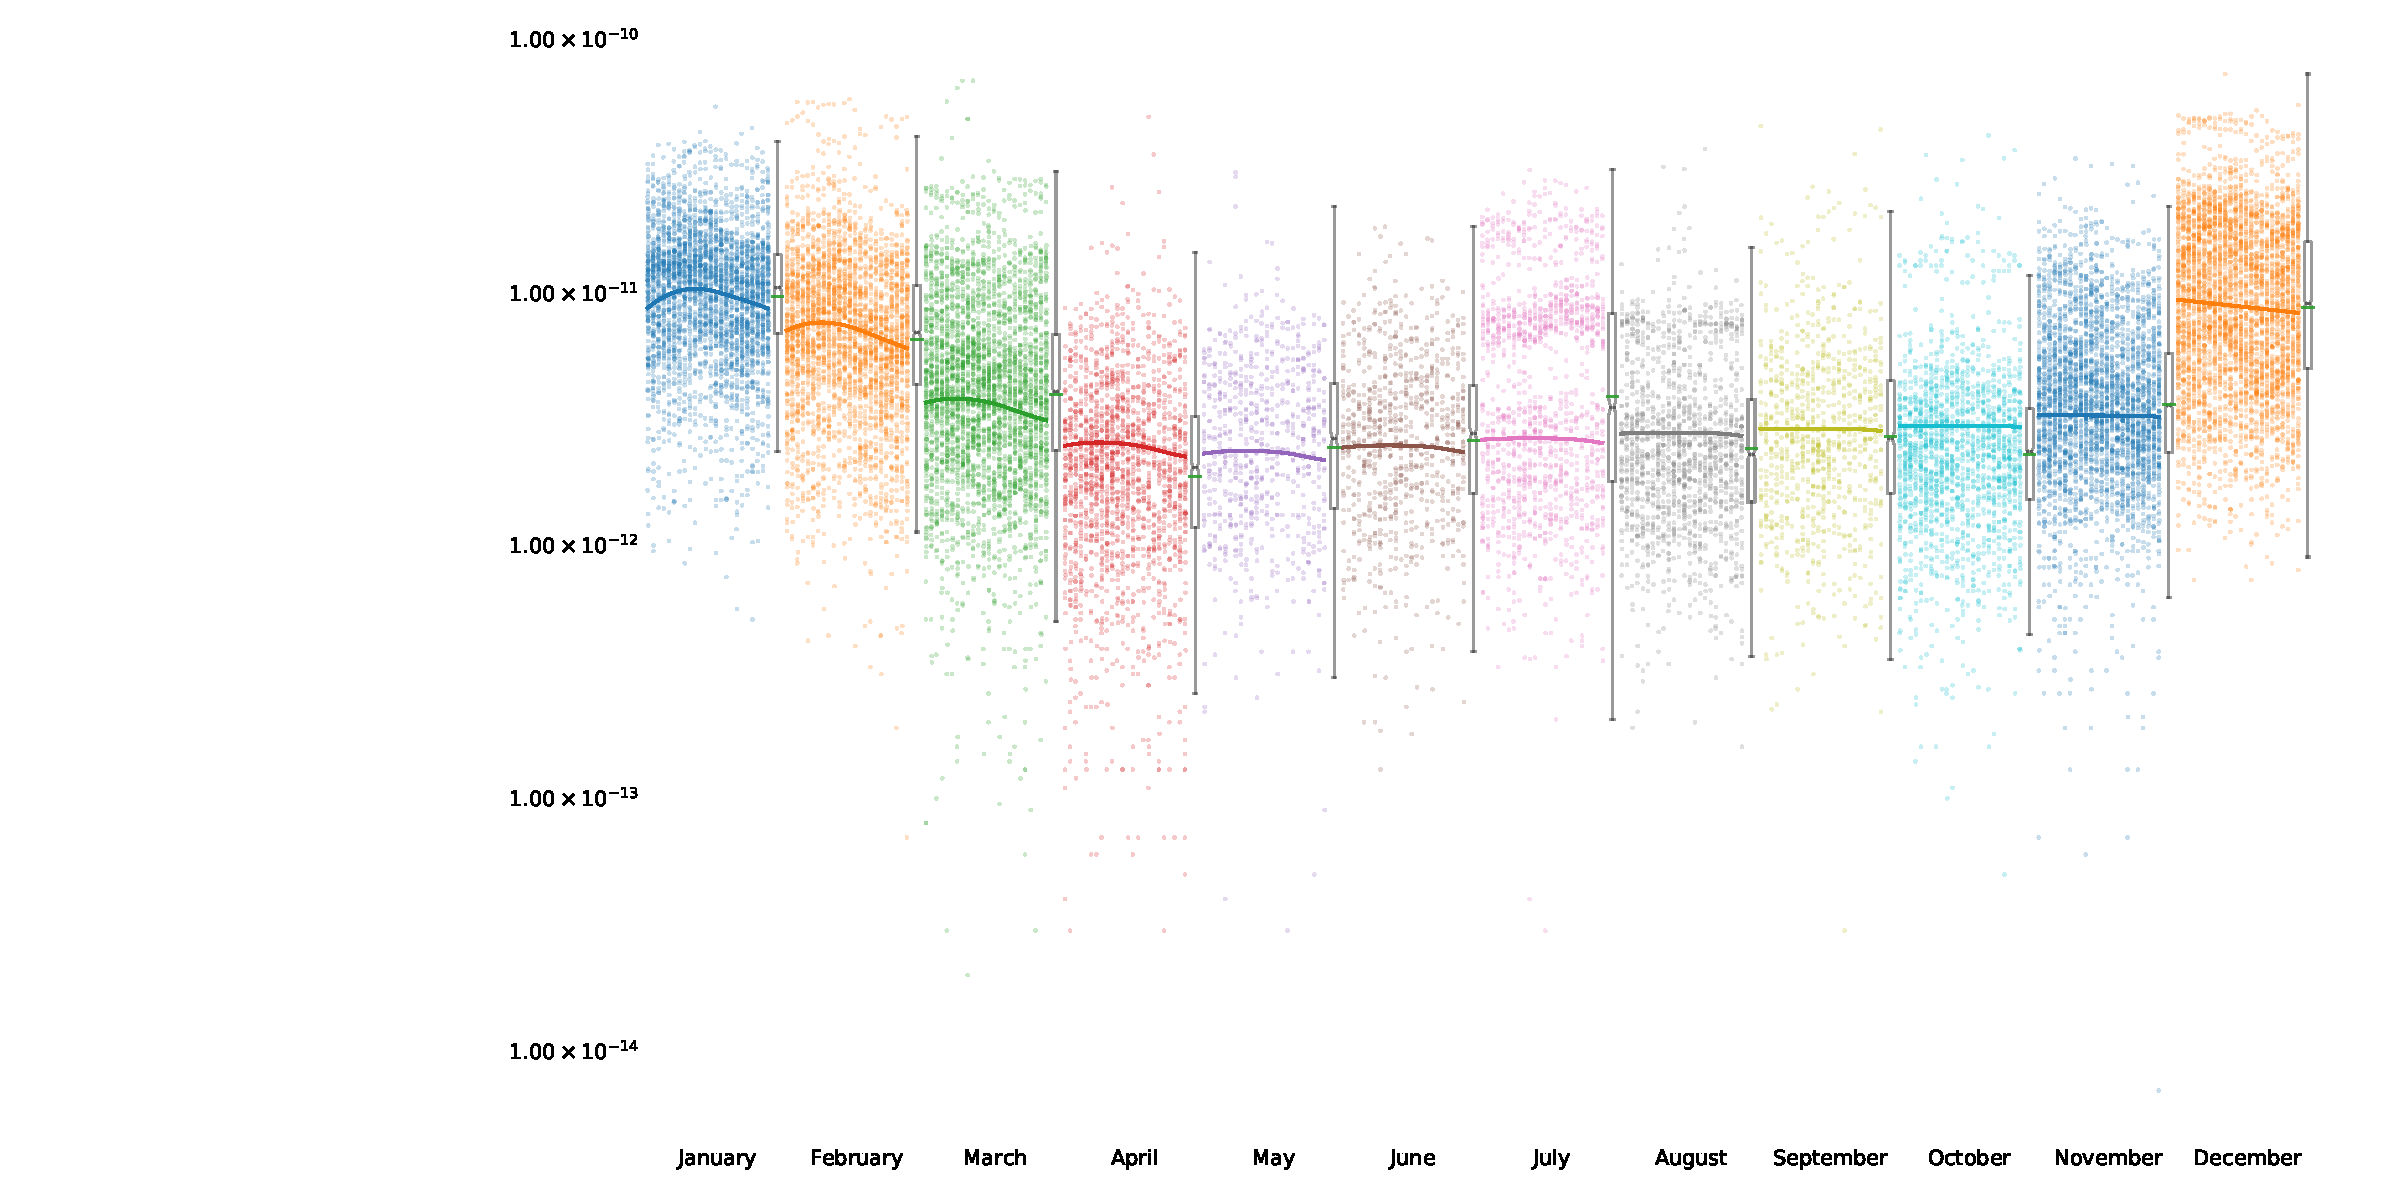
\includegraphics[width=.90\textheight,angle =90,trim={8cm 0 0 0}]{figures_c3/mlpregressor/CVNOX_CapeVerde/ISO_PENTANE.pdf}
        \caption{\textbf{Cape Verde MLP predicted and observational data of iso-Pentane.} Each segment represents data from a different month. Within each month segment exists 24 hour segments to create a diurnal. Observational concentrations are plotted in the form of a translucent scatterplot and summarised using the boxplot on the right of the month segment. MLP predicted results are shown using the solid lines. Concentration in mixing ratio. }
        \label{fig:mlpisopentane}
\end{figure}


\subsubsection{Model Initialisation Procedure}
The aim is to generate a set of initiation conditions which are representative of the species found for different environments around the world. In this section, we are not interested in the exact concentration modelling for specific times or scenarios. Instead, we seek to generate representative of the processed chemistry under a range of conditions.

Species concentrations are extracted from an MLP regressor trained on observational data for each scenario. Each concentration is that of noon local time from the generated diurnal from summer observations at each location. This produces a monthly error of $\pm 2 months$ from June. As both nitrogen oxide and dioxide are supplied, the total NO$_x$ for each simulation are \emph{not} constrained. The initial conditions are shown in \autoref{tab:icsmetric}.

In general observational measurements are not able to detect all the species presented within the MCM. This means that to be able to compare model scenarios, the chemistry must first be spun up. In propagating the chemistry forwards in time, primarily emitted and measured species are broken up forming the intermediate species which exist within a mechanism. To reach a steady-state, the model is initiated at noon, and the observational concentrations are rest every 24 hours. For each diurnal, the fractional difference between the concentrations at each day are compared. If the difference between these is less than 0.001, the model is left to run unconstrained for five days (right of the dashed line in \autoref{fig:cbeijing}). Model results are then taken after three days of unconstrained runs. The reason for this is that the total RO$_2$ concentration takes longer to stabilise in the polluted environments (London and Beijing). This falls into a periodic cycle beginning noon on the third day and can provide a representation of the processed chemistry within each environment.

\textit{NOTE: It should be noted that some of the concentration plots may appear to lose their diurnal dependability. This may be attributed to the changing order of magnitude of the concentrations, and that the species are still responding as expected. }

\subsubsection{Extracting The Required Results}
Model diagnostics such as concentration and the net flux passing through a species may be extracted directly from the DSMACC box model. These provide the baseline comparison and can be directly compared to the graph metrics. Species concentration tells us the abundance of different species, and the net-flux tells us how fast this is changing in time.

As some species may have a fast inwards and outwards flux (low net-flux), the absolute flux is also included. Finally, the sensitivity of each species for other species is also extracted (the Jacobian matrix). This serves to not only generate the graph used to represent the chemistry, (\autoref{sec:graphconstruction}) but also to identify the overall influence a species has on others in the network. This can be calculated by taking the net sum of the influence a species has on every other from the Jacobian. This is analogous to calculating the out-degree of a node in the Jacobian network.\\




\begin{table}[H]
\centering
\small

%%%%%%%
\begin{tabular}{p{0.2\textwidth}p{0.16\textwidth}p{0.16\textwidth}p{0.16\textwidth}p{0.16\textwidth}}
\toprule
Species & Beijing(APHH) & Borneo(OP3) &  London(ClearFlo) &  CapeVerde \\
\midrule
\ce{LAT}       & 39.9 &              0.96 &            51.0&       16.5 \\
\ce{LON}       &  116.3 &              114.5 &            0.00 &       23.4 \\
\midrule
CO & 3.829e-06 & 3.321e-07& 7.780e-09 & 0.0*\\
\ce{O3}        &  6.883e-08 &              8.939e-09 &            3.819e-08 &       2.629e-11* \\
\ce{NO}        &  1.660e-09 &              2.668e-14* &            2.350e-09 &       2.358e-12 \\
\ce{NO2}       &  1.226e-08 &              1.081e-13* &            7.445e-09 &       8.447e-12 \\
\ce{HCHO}      &  4.472e-09 &                        &            1.119e-08 &                 \\
\ce{C2H6}      &  3.163e-09 &              7.315e-10 &            2.133e-09 &       4.539e-10 \\
\ce{C2H4}      &  1.004e-09 &              1.152e-10 &            4.893e-10 &       2.481e-11 \\
\ce{C3H8}      &  3.019e-09 &              1.924e-10 &            1.128e-09 &       1.728e-11 \\
\ce{C3H6}      &  1.335e-10 &              1.333e-11 &            1.784e-10 &       9.343e-12 \\
\ce{IC4H10}    &  6.412e-10 &              8.742e-11 &            5.142e-10 &       2.486e-12 \\
\ce{NC4H10}    &  1.593e-09 &              5.698e-11 &            1.058e-09 &       4.481e-12 \\
\ce{C2H2}      &  1.058e-09 &              1.825e-10 &            3.018e-10 &       1.848e-11 \\
{TBUT2ENE}  &  4.198e-11 &                        &            1.815e-11 &                 \\
{CBUT2ENE}  &  4.454e-11 &                        &            1.305e-11 &                 \\
\ce{IC5H12}    &  1.047e-09 &              2.883e-11 &            7.424e-10 &       3.470e-12 \\
\ce{NC5H12}    &  4.650e-10 &              2.090e-11 &            2.792e-10 &       2.513e-12 \\
{TPENT2ENE} &  3.939e-11 &                        &                      &                 \\
{CPENT2ENE} &  3.982e-11 &                        &                      &                 \\
\ce{NC6H14}    &  2.057e-10 &              6.437e-12 &            6.357e-11 &                 \\
\ce{C5H8}      &  7.134e-10 &              1.957e-09 &            1.640e-10 &                 \\
\ce{NC7H16}    &  7.905e-11 &                        &            5.222e-11 &                 \\
\ce{BENZENE}   &  4.045e-10 &                        &            1.137e-10 &       7.682e-12 \\
\ce{NC8H18}    &  3.091e-11 &                        &            1.442e-11 &                 \\
\ce{TOLUENE}   &  6.767e-10 &                        &            3.205e-10 &       3.121e-12 \\
\ce{EBENZ}     &  3.115e-10 &                        &            6.017e-11 &                 \\
\ce{OXYL}      &  1.677e-10 &                        &            5.049e-11 &                 \\
\ce{CH3CHO}    &  4.783e-10 &                        &            4.095e-09 &                 \\
\ce{C2H5OH}    &  4.655e-09 &                        &            3.125e-09 &                 \\
\ce{CH3COCH3}  &  3.328e-09 &                        &            2.924e-09 &                 \\
\ce{NC9H20}    &  1.336e-11 &                        &            7.922e-11 &                 \\
\ce{NC10H22}   &  1.062e-12 &                        &            1.602e-10 &                 \\
$\alpha$-\ce{PINENE}\footnotemark
   &  7.341e-11 &     15e-11                   &            1.105e-10 &                 \\
\ce{LIMONENE}  &  5.836e-11 &              1.351e-10 &            3.566e-11 &                 \\
\ce{PXYL+MXYL}\footnotemark
 &  4.943e-10 &                        &                      &                 \\
\ce{IPBENZ}    &  4.567e-10 &                        &                      &                 \\
\ce{PBENZ}     &  3.996e-10 &                        &                      &                 \\
\ce{HONO}      &  6.479e-10 &                        &            4.109e-10 &                 \\
\ce{MACR}      &            &              6.948e-11 &            1.862e-11 &                 \\

%%%%%%%%%%%%%%%
\bottomrule
\end{tabular}
\end{table}


\begin{table}[H]
\centering
\small
\begin{tabular}{p{0.2\textwidth}p{0.16\textwidth}p{0.16\textwidth}p{0.16\textwidth}p{0.16\textwidth}}
\toprule
Species & Beijing(APHH) & Borneo(OP3) &  London(ClearFlo) &  CapeVerde \\
\midrule

%%%%%%%%%%%%%%

{PENT1ENE}  &            &                        &            2.383e-11 &                 \\
\ce{MVK}       &            &                        &            2.091e-11 &                 \\
\ce{NPROPOL}   &            &                        &            2.883e-10 &                 \\
\ce{NBUTOL}    &            &                        &            4.535e-10 &                 \\
\ce{STYRENE}   &            &                        &            2.241e-11 &                 \\
\ce{MEK}       &            &                        &            5.494e-11 &                 \\
\ce{C3H7CHO}   &            &                        &            9.534e-12 &                 \\
\ce{C4H9CHO}   &            &                        &            1.865e-11 &                 \\
\ce{C5H11CHO}  &            &                        &            1.201e-11 &                 \\
\ce{CYHEXONE}  &            &                        &            9.790e-12 &                 \\
\ce{BENZAL}    &            &                        &            1.510e-11 &                 \\
\ce{PAN}       &            &                        &            1.791e-10 &                 \\
\bottomrule
\end{tabular}


\caption{(2-page split) The initial conditions created from the MLPRegressor prediction of observational data. Although not specified the mixing ratios for methane is set by the model at 1770ppb, the temperature is 298K, and water vapour is at 2\%. \textbf{* Starred values are of the wrong units and should be multiplied by 1000. As there was no time to rerun these, their results have been omitted from this chapter.}}
\label{tab:icsmetric}
\end{table}

\footnotetext{This is (incorrectly) written as `?-pinene' in the merged CEDA dataset for the Borneo OP3 campaign. This is due to character conversion errors.}
\footnotetext{The mixing ratios for these is split evenly between both species}

%

%
%
%



\begin{figure}[H]
    \centering
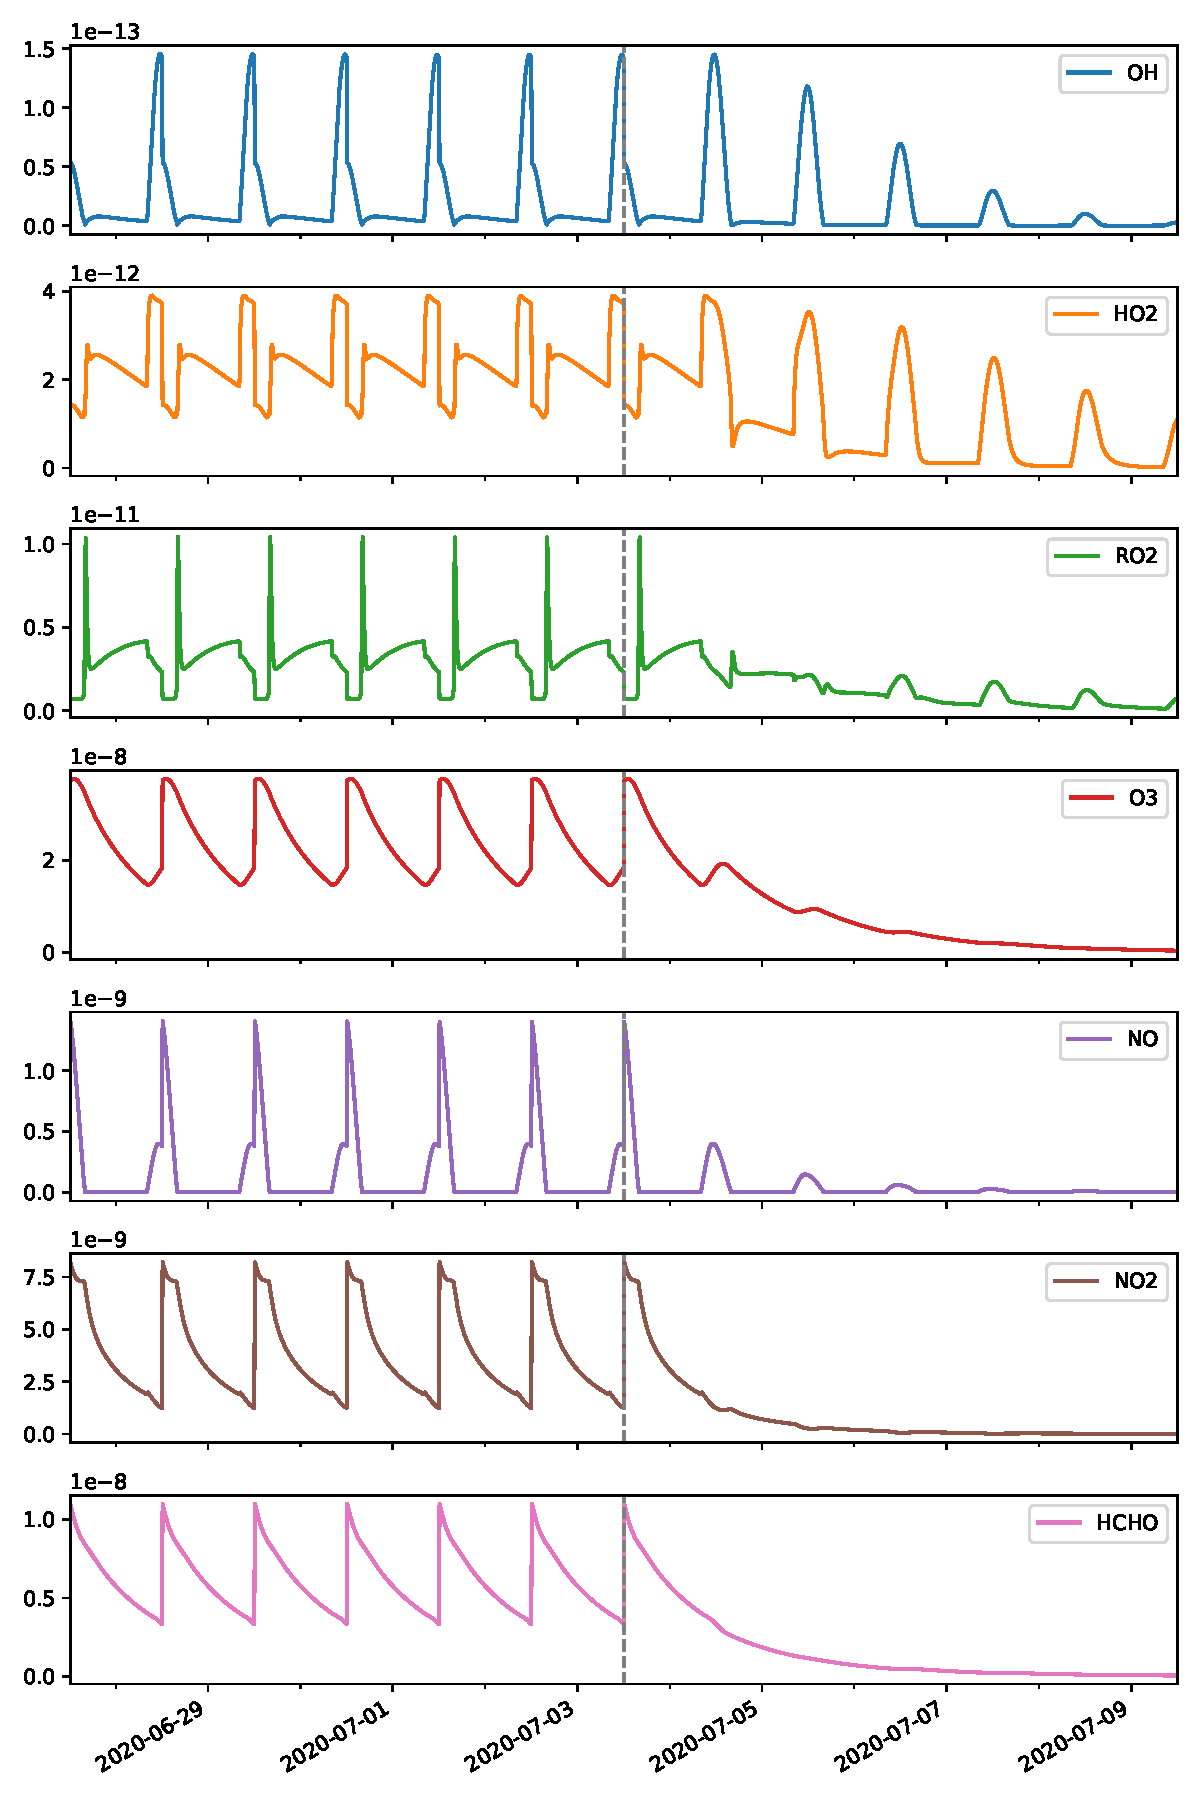
\includegraphics[width=.9\textwidth]{figures_c3/mlpregressor/conc_clfo.pdf}
\caption{\textbf{The mixing ratio profile for London.}This shows a the change in mixing ratio over time for HO$_x$,NO$_x$, HCHO,Ozone and RO$_2$ species for a simulation run generated by the mlpregressor. Left of the dashed line shows the last 6 days of spinup, where the values are reset at noon each day until the species fractional difference is less than 0.001 .}
\label{fig:clondon}
\end{figure}

\newpage


\begin{figure}[H]
    \centering
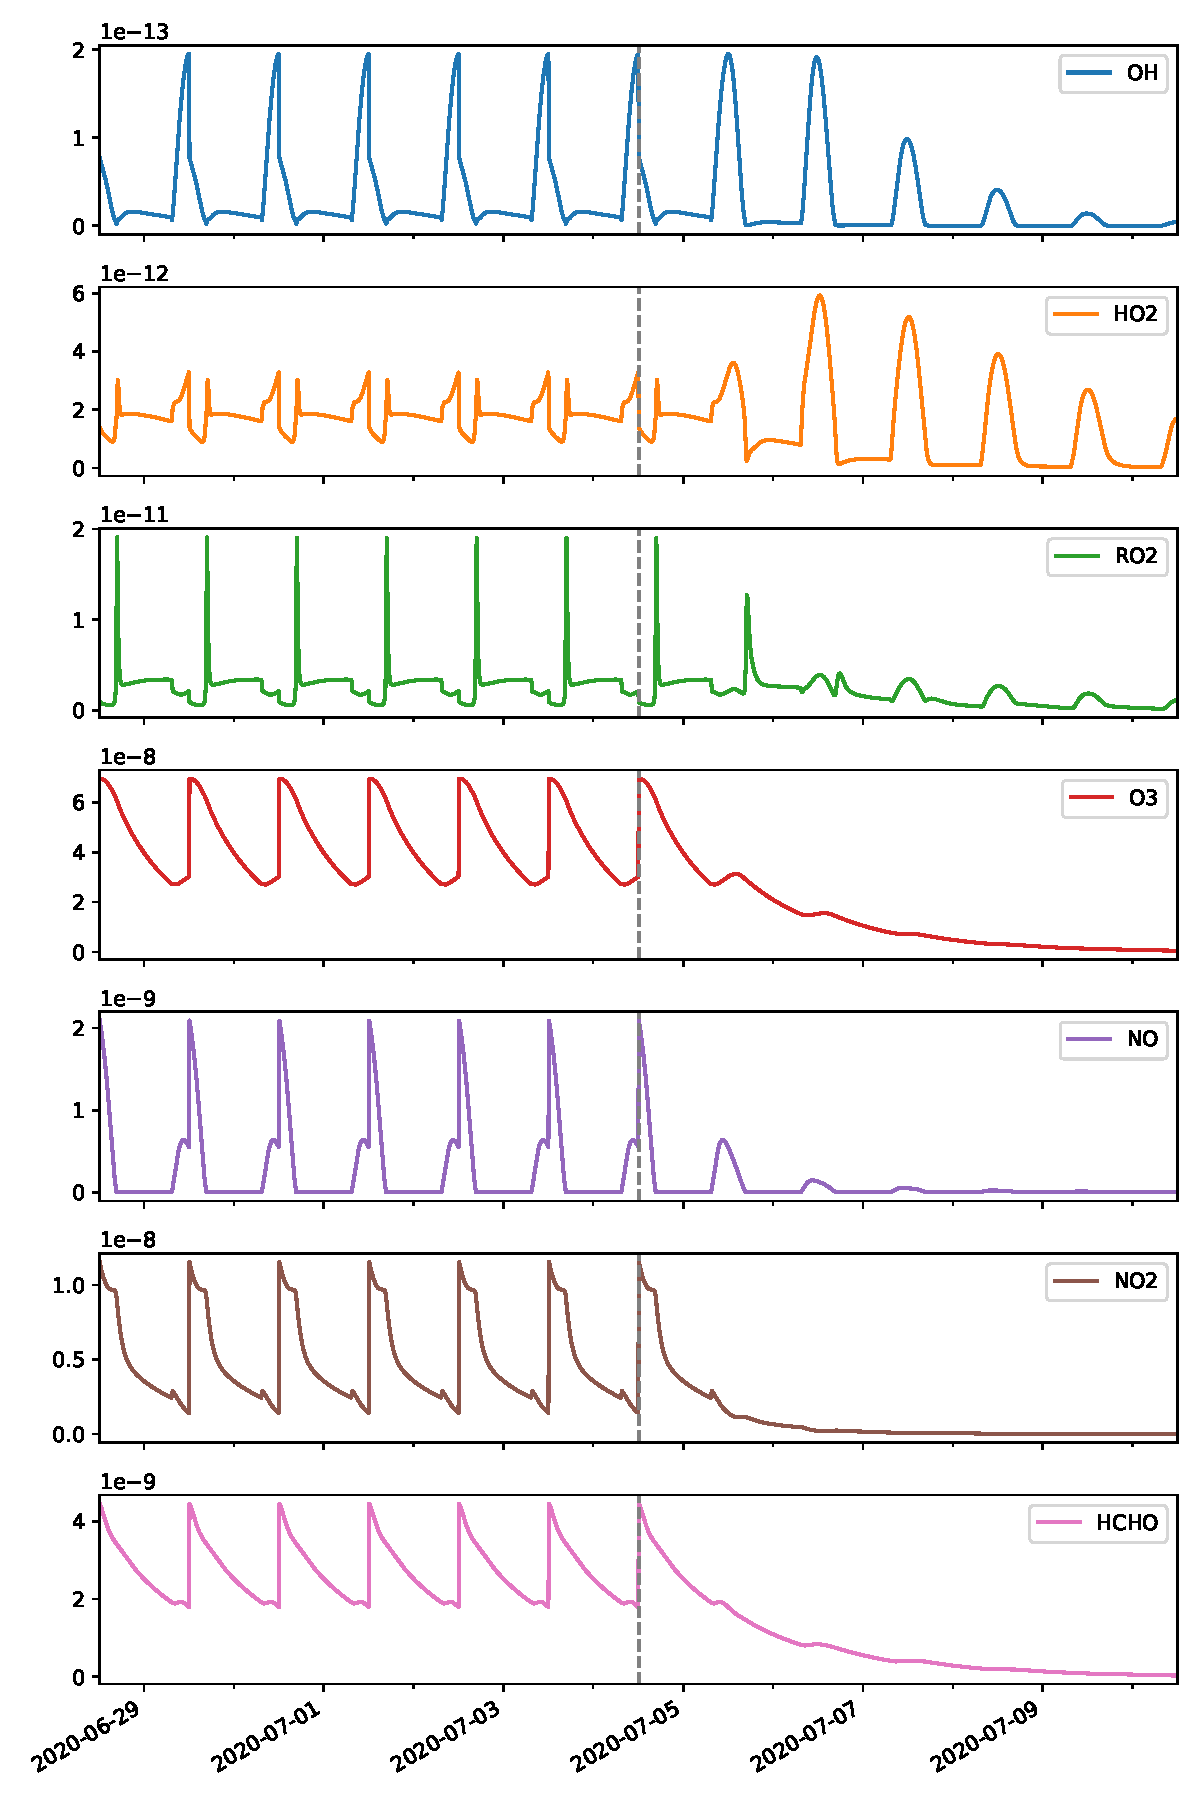
\includegraphics[width=.9\textwidth]{figures_c3/mlpregressor/conc_beijing.pdf}
\caption{\textbf{The mixing ratio profile for Beijing.}This shows the change in mixing ratio over time for HO$_x$, NO$_x$, HCHO, Ozone and RO$_2$ species for a simulation run generated by the MLPRegressor. Left of the dashed line shows the last six days of spinup, where the initial values are reset at noon each day until the species fractional difference is less than 0.001 .}\label{fig:cbeijing}
\end{figure}

\newpage





\subsubsection{Unifying The Results}
Each metric provides a different range in which it ranks the importance of a node. All results are scaled to the range \{0,1\}, where one is the highest. Entries, where the results span several orders of magnitude (e.g. concentration, flux, influence), are flattened using the $\log_{10}$ scale before being normalised.



\subsection{Comparing Results}
This subsection juxtaposes the use of traditional model diagnostic methods against a selection of graph metrics. As there are several thousand species within each simulation run, the keyword extraction algorithm Term Frequency - Inverse Document Frequency (TF-IDF), is used to identify the top most prominent species for each metric (traditional and graph). From this, the ten highest-ranking species from each category are collated into a single diagram for comparison.


\subsubsection{What Is TF-IDF}
TF-IDF is a numerical statistic used in text natural language processing and text mining. It is designed to identify the importance of a word concerning its context.

It provides a value for the frequency a word appears within a document, offset by the number of times it appears in other documents within the corpus - It is for this reason that 83\% of text recommender systems in digital libraries use TF-IDF, \citep{tf83}.

 In \citep{frankenstein} this was applied this to the chapters of Frankenstein and found the keywords extracted almost exactly replicated those from the synoptic description of the novel. Although TF-IDF is a text mining procedure, the algorithm itself is mathematical, meaning that it may be applied to our diagnostic dataset. The working of the algorithm is discussed below.

\paragraph*{Term frequency}
The TF from the algorithm name stands for term frequency. This is an analysis of the number of times a word exists within a dataset. There are several ways in which this can be done; these are:

\begin{itemize}
    \item[-] \textbf{Raw Count} - The \textit{number of times} a word exists within the document.
    \item[-] \textbf{Boolean/Logistic} - $True$ if the word exists, false otherwise.
    \item[-] \textbf{Adjusted for Document Length} -  $word\ frequency / total\ number\ of\ words$
    \item[-] \textbf{Log Scaled} - $\log(1+frequency)$
\end{itemize}

As the scaled values for each item are taken, we can liken our results to the `Adjusted for Document length' equation and use the scaled ranking value for each group.

\paragraph*{Inverse Document Frequency}
Inverse document frequency tells us how much information a word provides concerning a specific context. While a word may be used extensively throughout a set of documents (a corpus) -  (i.e. term frequency), often that we are interested in the words which frequently appear only within an individual document. This is one of the reasons TF-IDF is useful in the extraction of keywords from a document.

The inverse frequency of a word is usually calculated as the $\log$ of the number of documents ($N$) divided by the number of documents the word appears in ($D_f$), \autoref{eqn:idf}.


\begin{equation}
    IDF = \log(\frac{N}{D_f})
    \label{eqn:idf}
\end{equation}

If required, changes can be made to produce results which show a better representation of words which are important in all documents (probabilistic, \autoref{eqn:idfprob}) or individually (smooth, \autoref{eqn:idfsmooth}). However in looking at \autoref{fig:idf}, it can be seen that the basic IDF formula mentioned has a limit of zero the higher the document frequency ($D_f$), which makes it easy to normalise against (divide by 2) as this is the value tended to if the document frequency tends to 0.


\begin{equation}
    IDF_{prob} = \log(\frac{N-D_f}{D_f})
    \label{eqn:idfprob}
\end{equation}

\begin{equation}
    IDF_{smooth} = \log(\frac{N}{1+D_f})+1
    \label{eqn:idfsmooth}
\end{equation}


To complete the TF-IDF equation, the frequency terms and inverse document frequency terms are multiplied together.

\paragraph*{Applying TF-IDF to chemical metrics}
To identify metrics selection criteria, we seek only species (words) which are important only for that metric. The TF-IDF algorithm can be adapted for use with the graph metric output. Here `Term Frequency' corresponds to the number of times a value appears within the body of a document and can be seen as the scaled \{0,1\} metric output. This is then divided by the log of the `Inverse Document Frequency'.  $D_f$ is the sum of values across all the metrics. This makes the TF-IDF equation:

\begin{equation}
    TF.IDF = metric\_value\  .\ \log(\frac{N_o\ documents}{ \Sigma_\forall\ metric\_values})
\end{equation}


\begin{figure}[H]
     \centering
         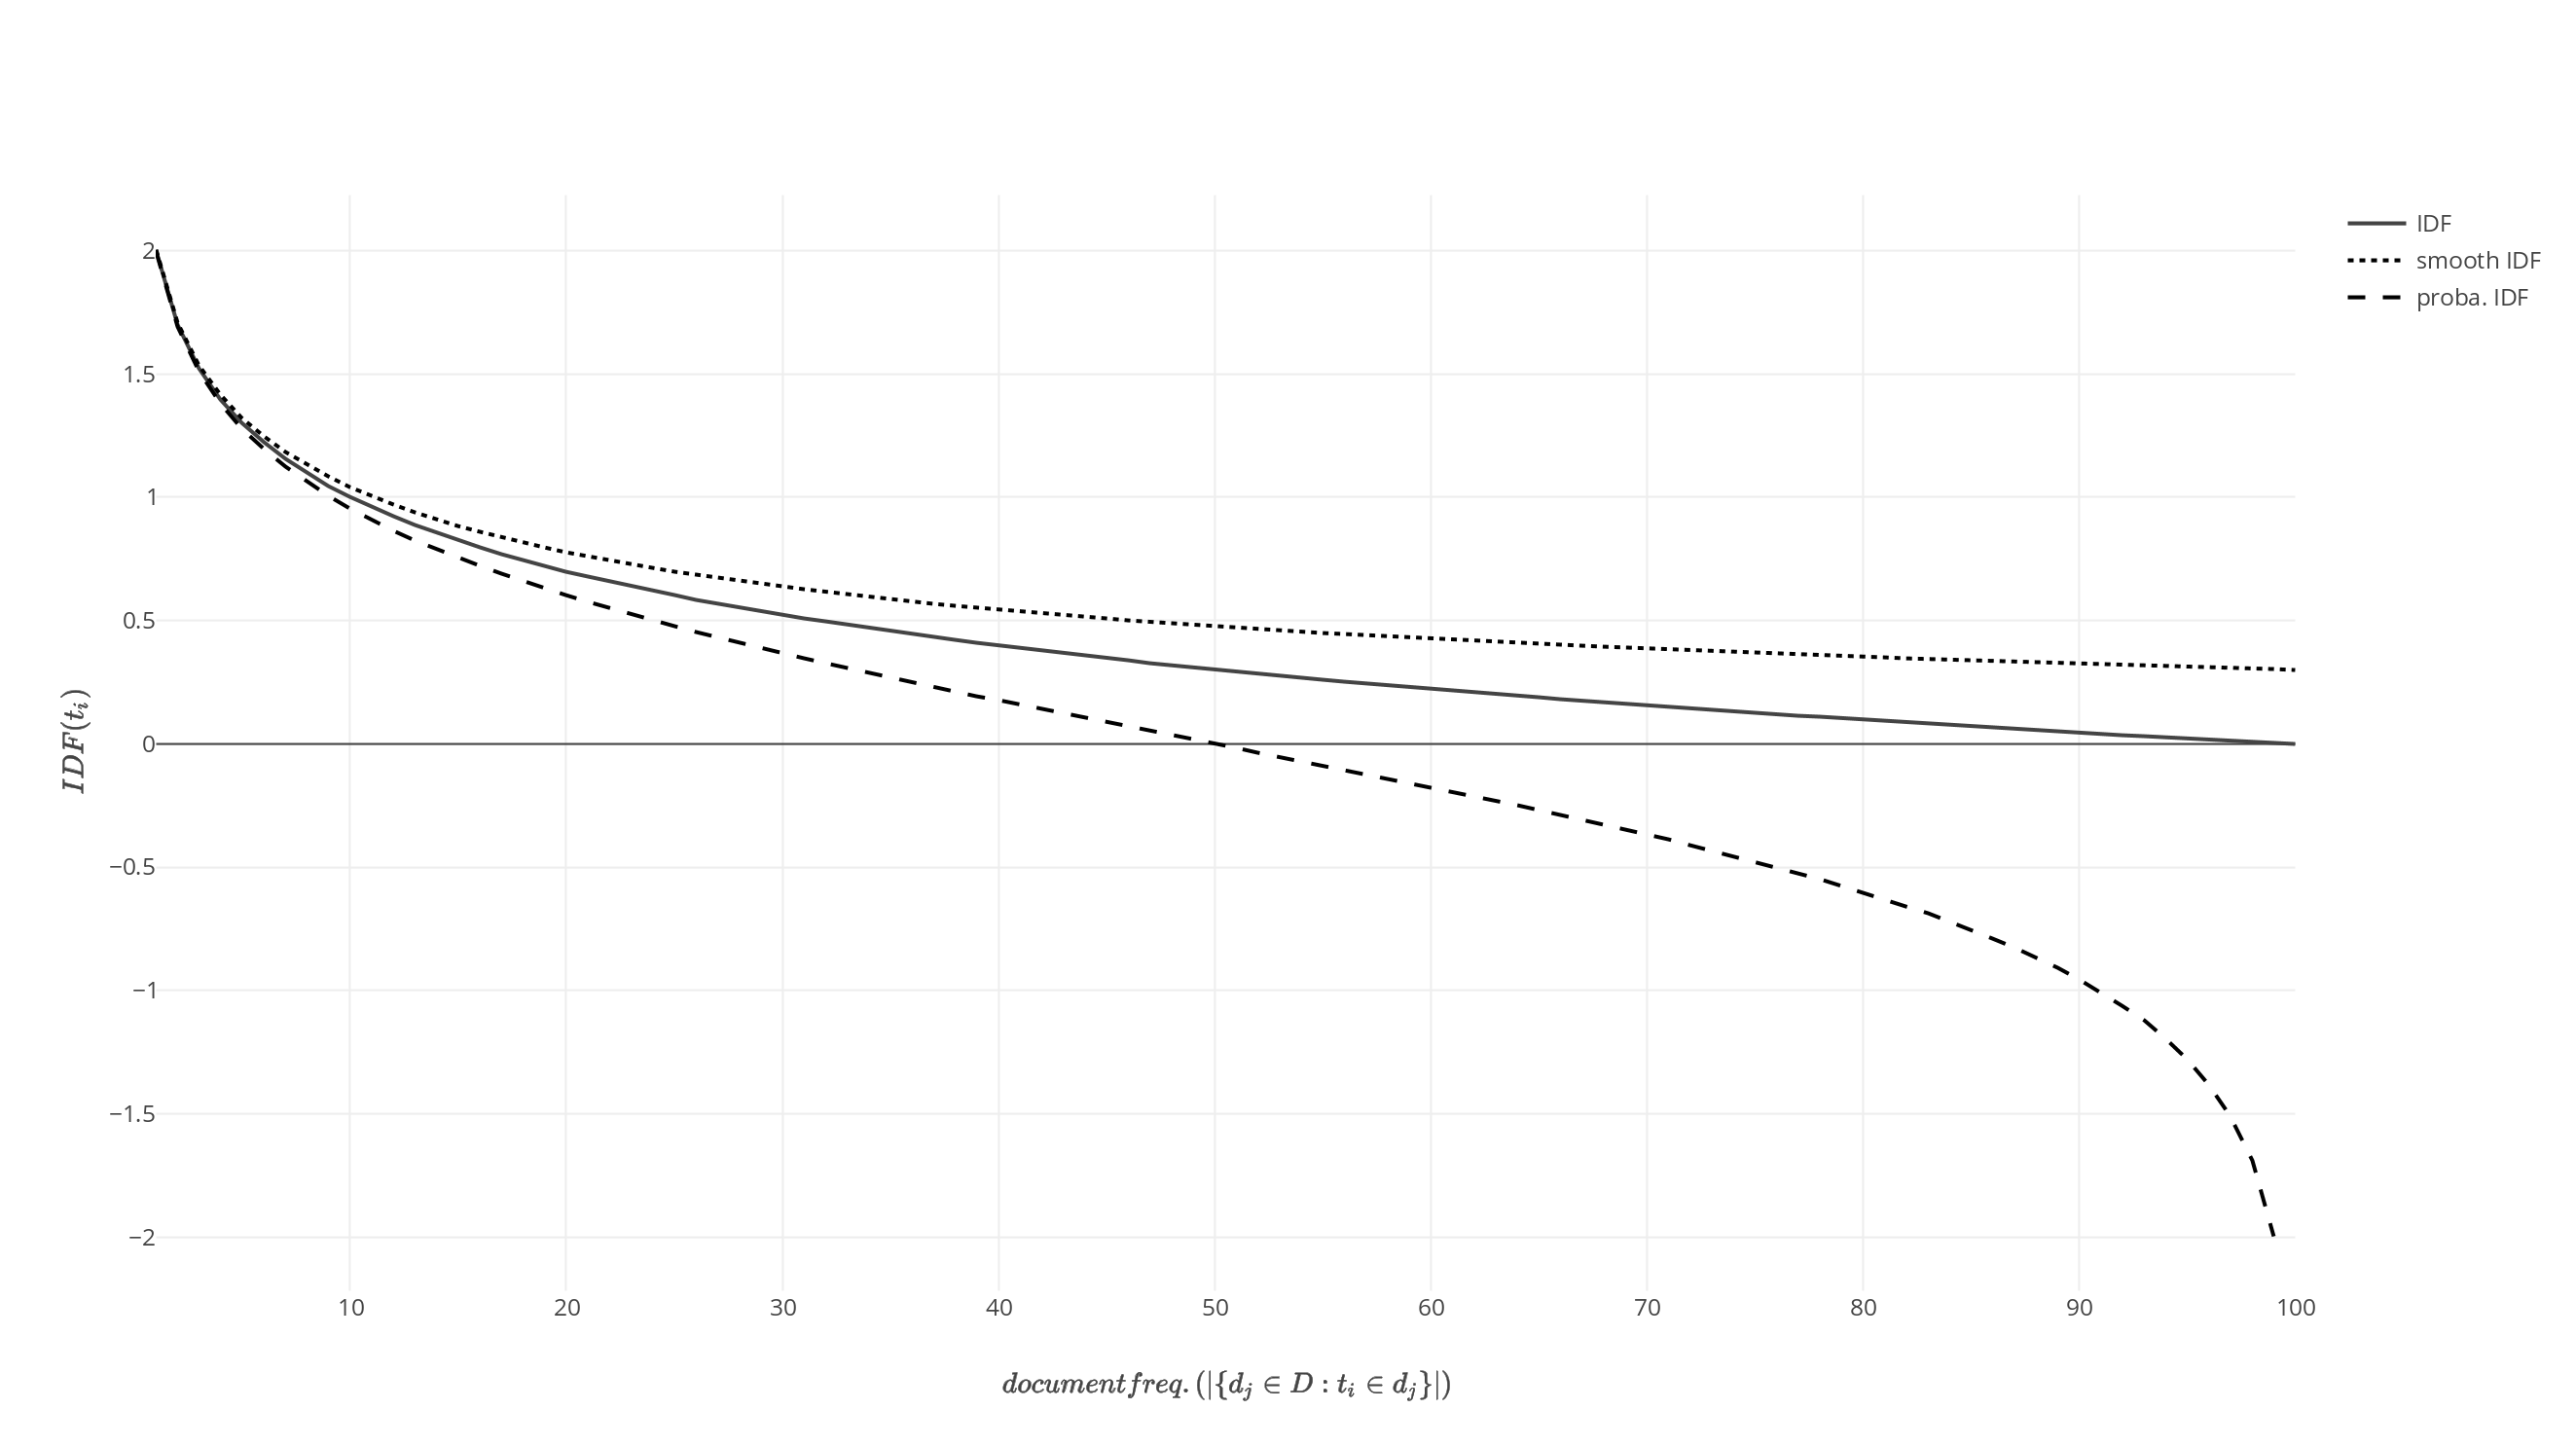
\includegraphics[width=\textwidth]{figures_c3/mlpregressor/plotidf.png}
        \caption{ \textbf{The different IDF outputs.} A plot showing Inverse Document Frequency profiles against Document Frequency. This shows that the probabilistic IDF highlights words that are more important across all items, while the smooth IDF shows files which are more important individually. The general IDF (which is used) produces a result starting at two and tending to zero. This provides the best response and can easily be scaled between the range of [0,1] by dividing the output by 2.  Source: \citep{idfpic}}
        \label{fig:idf}
\end{figure}




\subsubsection{Metric Comparison}

This section aims to compare the efficiency of graph metrics against a list of traditional methods in determining species which play an important role within the network. To do this a bivariate colourmap (\autoref{fig:cmap}) is used. Each figure consists of a red-hued image/heatmap representing the scaled values \{0,1\}:\{white, red\} for each of the individual metrics (graph columns). As each simulation contains thousands of species, only the top 10 species from each column/category are selected. These are then sorted by the average sum of their closeness, betweenness and page-rank values (blue column). Superimposed on this reds-only heatmap is a blue heatmap representing the average sum of the three metrics for comparison. Such a method allows for the comparison of individual values against an approximation of species importance, by the sum of graph metrics - allowing an easy categorisation of the data:

\begin{itemize}
\item[-] \textbf{Purple} - This value is high in both the individual category and the metric sum.
\item[-] \textbf{Red} - This value is high for the individual category but not the metric sum.
\item[-] \textbf{Blue} - This value is high for the metric sum but not the individual category.
\item[-] \textbf{White} - This value is low for all categories.
\end{itemize}



\begin{figure}[H]
     \centering
         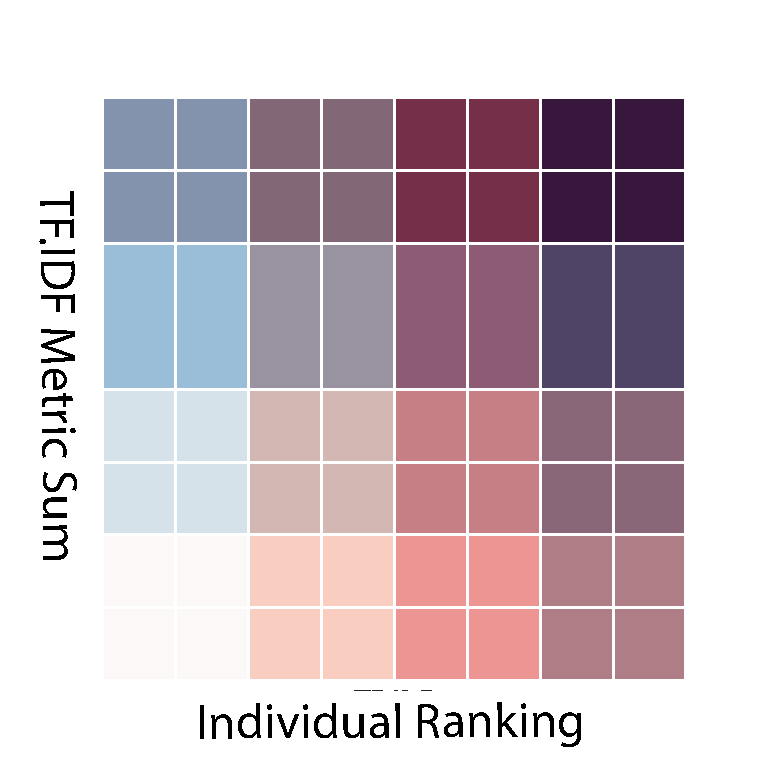
\includegraphics[width=0.35\textwidth,angle=45]{figures_c3/mlpregressor/cbar.pdf}
        \caption{ \textbf{The bivariate colourplot key.} }
        \label{fig:cmap}
\end{figure}


\subsubsection{Individual Categories}
Individual categories are split between traditional metrics and graph centrality metrics. To represent the importance of a species, the following values may be extracted through the use of a simple box model:

\begin{itemize}
\item[-] \textbf{Concentration} - this describes the abundance of a species within the atmosphere.
\item[-] \textbf{Net flux} - this describes the rate of net (absolute) change of concentration over time for a species.
\item[-] \textbf{Absolute flux} - some species may have a large flux going through them (production and loss), resulting in a small net flux. This sums the production and loss fluxes.
\item[-] \textbf{ influence} - influence is the total magnitude of an effect that changing a species concentration by 1\% would have on other species within the network. Since the graph is generated using the Jacobian matrix, an alternative method for calculating this can be by calculating the total out-degree of a node.
\end{itemize}



The importance of a species is then compared through the use of three of the most common centrality metrics. These are:


\begin{itemize}
\item[-] \textbf{Closeness} - This describes how easily information from one node can be disseminated to all other nodes (see \autoref{sec:closeness}).
\item[-] \textbf{ betweenness} - This describes the number of shortest paths (fastest fluxes/greatest influences) that are routed between nodes adjacent to our chosen node. Species with a high betweenness hold a brokering position and can act as a bottleneck between different groups of chemistry (see \autoref{sec:betweenness}).
\item[-] \textbf{PageRank} - PageRank looks at the flow in a system. It ranks nodes not only on the number of species it reacts with but also the importance of the species it has reacted with (see \autoref{sec:pagerank}).

\end{itemize}

Finally, the `Metric Sum' is the sum of all the metric values scaled between 1 and zero (the mean).

\subsection{Scenario Analysis}
In selecting the top 10 ranking species for each category, it is possible to examine if the importance of a species with centrality metrics varies from the results suggested by traditional metrics. In this subsection, we explore the TF-IDF rankings of each metric and use this to decide if species importance is local to a specific metric. We look at what species are highlighted by each scenario (Figures \ref{fig:heatl} - \ref{fig:heatbj}) and compare them against the primary emitted species shown in \autoref{tab:icsmetric}. Finally, we compare the total metric sum against the traditional metrics of concentration and flux and compare the correlation.
%
%
%

%


\subsection*{London}
The London dataset (\autoref{fig:fglondon}) contains a mix of anthropogenic and biogenic aromatics and long-chain alkanes. We have a section of alkanes which have a low overall metric sum and a small value for closeness and page rank. Combined with their high net flux, absolute flux and influence values, this suggests that they have a moderate directional flux, most likely influencing the production of many other species at a consistent rate. In addition to these, we have species with a moderate closeness but a high betweenness. These are often species such as formaldehyde (\ch{HCHO}), glyoxal and acetaldehyde which can serve as tracers for fast photolytic reactions. This is because on the graph structure (\autoref{fig:vk}) they sit between the dense centre of the network (high closeness) and the branches formed from each primary emitted species (a low closeness value). Their high connection density and importance in the network is also picked up by the page rank algorithm. Other species with high betweenness and a low centrality are the monoterpenes limonene and $\alpha$ pinene, as well as hexane (\ch{nc6h14}) and butane products. These are (or are close to) primary emitted species and therefore have a low closeness. Since much of the chemistry originates with such species, the outward `flow' of information also results in a lower page rank value.

\begin{figure}[H]
     \centering
         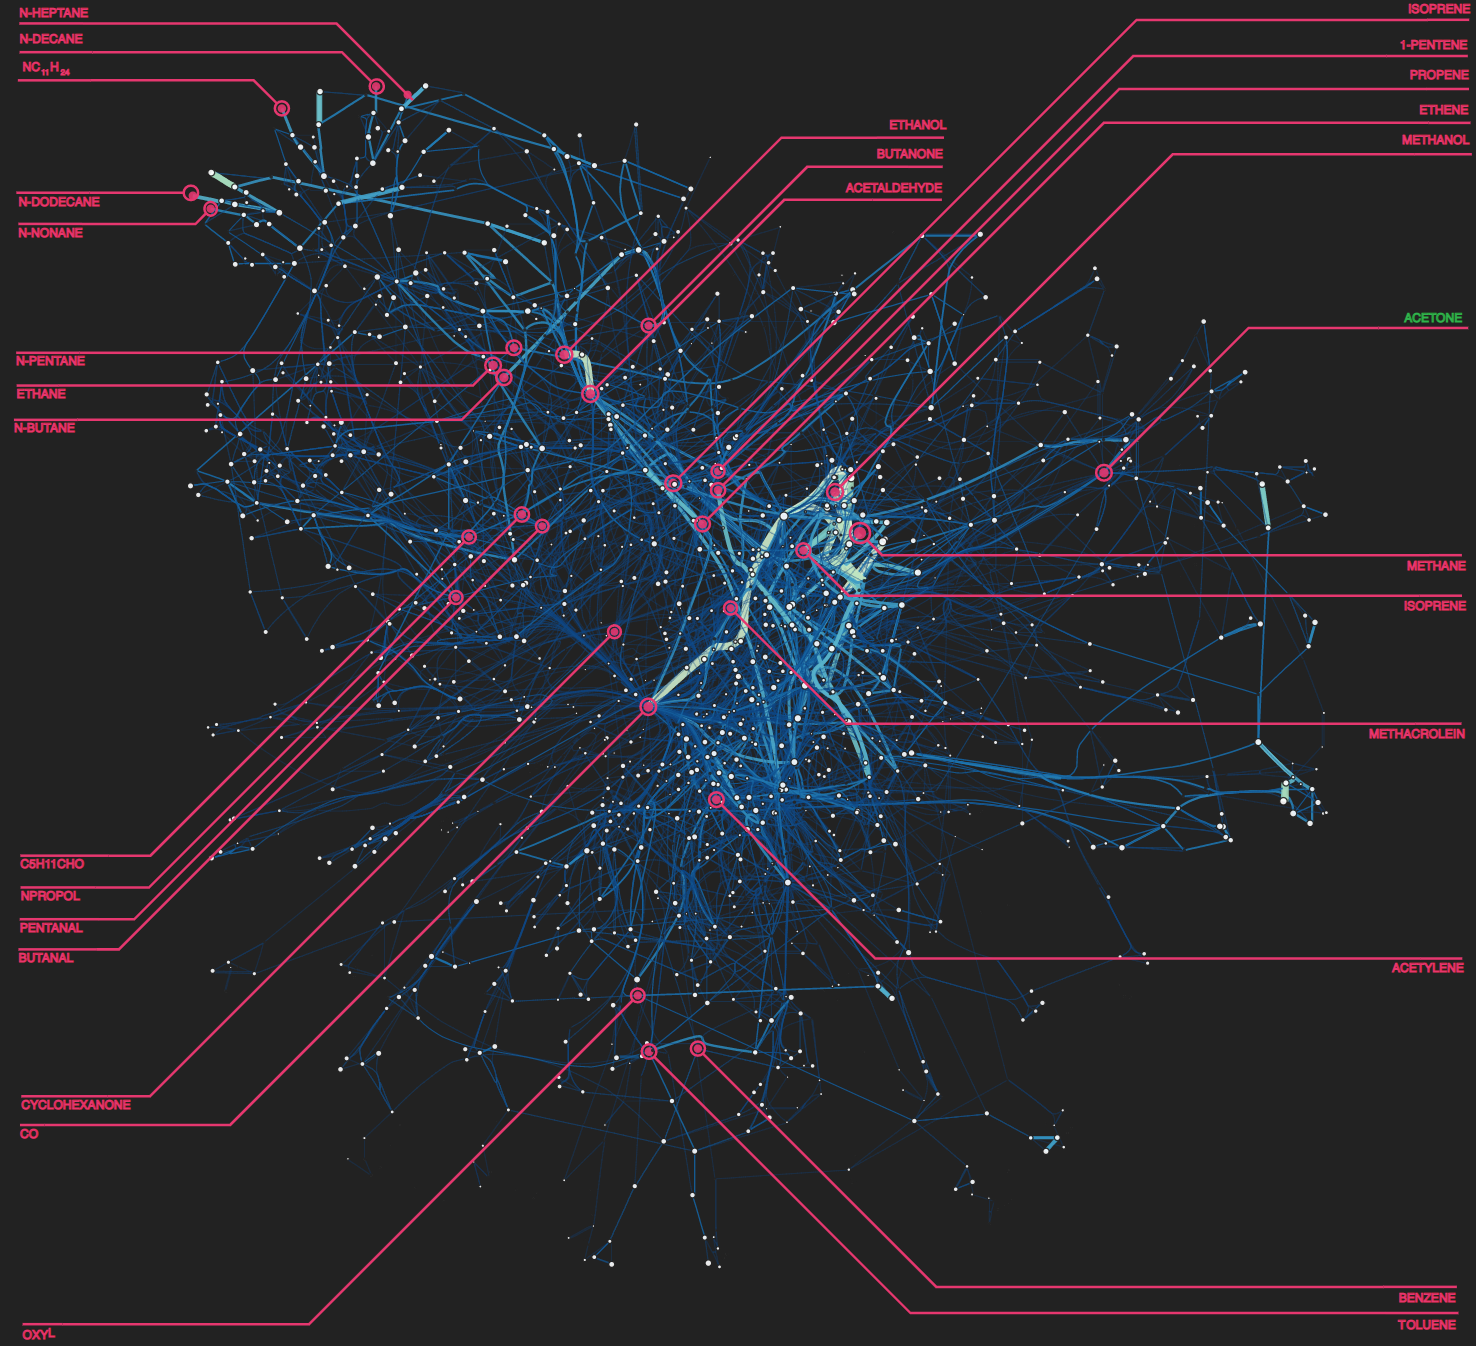
\includegraphics[width=.95\textwidth]{figures/lewis.png}
        \caption{ \textbf{An example force graph showing the complex chemistry of London.} (Weightings not from initial conditions described.) Source: \citep{science}  }
        \label{fig:fglondon}
\end{figure}



\subsection*{Beijing}


Similar to London, the fast photochemical tracers are identified, although some have a slightly lower flux between them (Betweenness) and page rank values for Beijing (\autoref{fig:fgbeijing}). This suggests that the network structure or weightings may have shifted slightly from London, creating more links, or importance in a specific branch of chemistry.
 Additionally, their overall metric sum is lower. Glyoxal, Methyl Vinyl Ketone (MVK) and their associated criegee configurations all feature heavily in the middle of \autoref{fig:heatbj}. These are important as they represent the fast chemistry formed by both the anthropogenic and biogenic chemistry that is within the simulation. These tend to have a high closeness and page rank centrality, a pattern that is also seen with the long-chain alkane products from Octane (n-\ch{C8H18}), Hexane (n-\ch{c6h14}) and Isoprene.

 \begin{figure}[H]
      \centering
          \includegraphics[width=.95\textwidth]{figures/paperbeijingnight.pdf}
         \caption{ \textbf{An example force graph showing the complex chemistry of Beijing.} (Weightings not from initial conditions described.)}
         \label{fig:fgbeijing}
 \end{figure}
%

\begin{figure}[H]
     \centering
         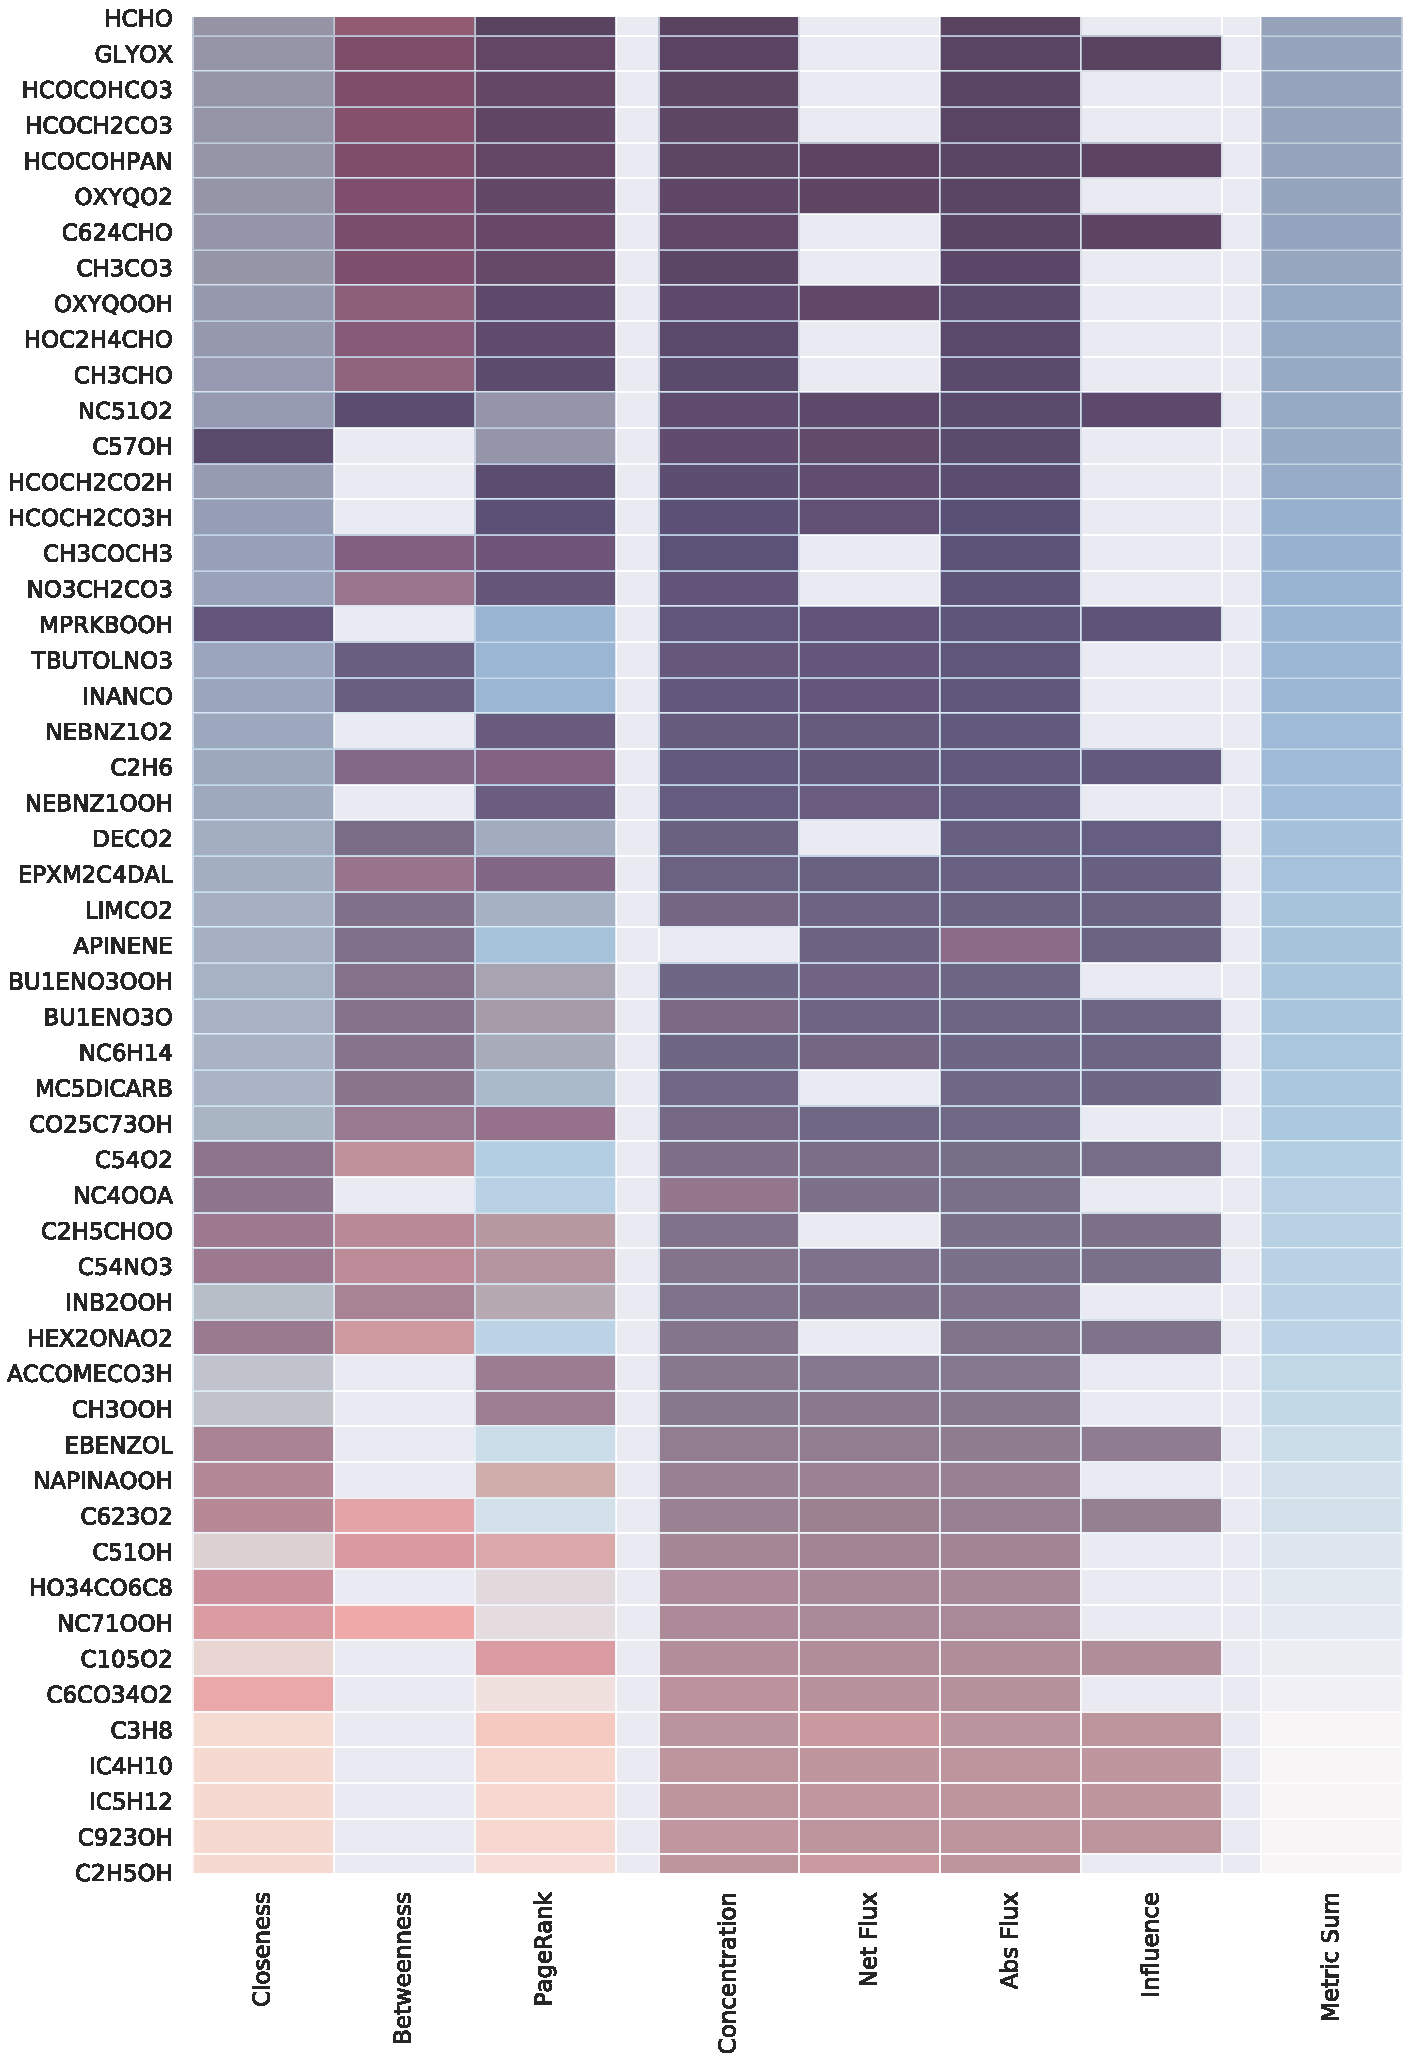
\includegraphics[width=.95\textwidth]{figures_c3/mlpregressor/clfo_London.pdf}
        \caption{ \textbf{A bivariate heatmap comparison of London.} }
        \label{fig:heatl}
\end{figure}

\begin{figure}[H]
     \centering
         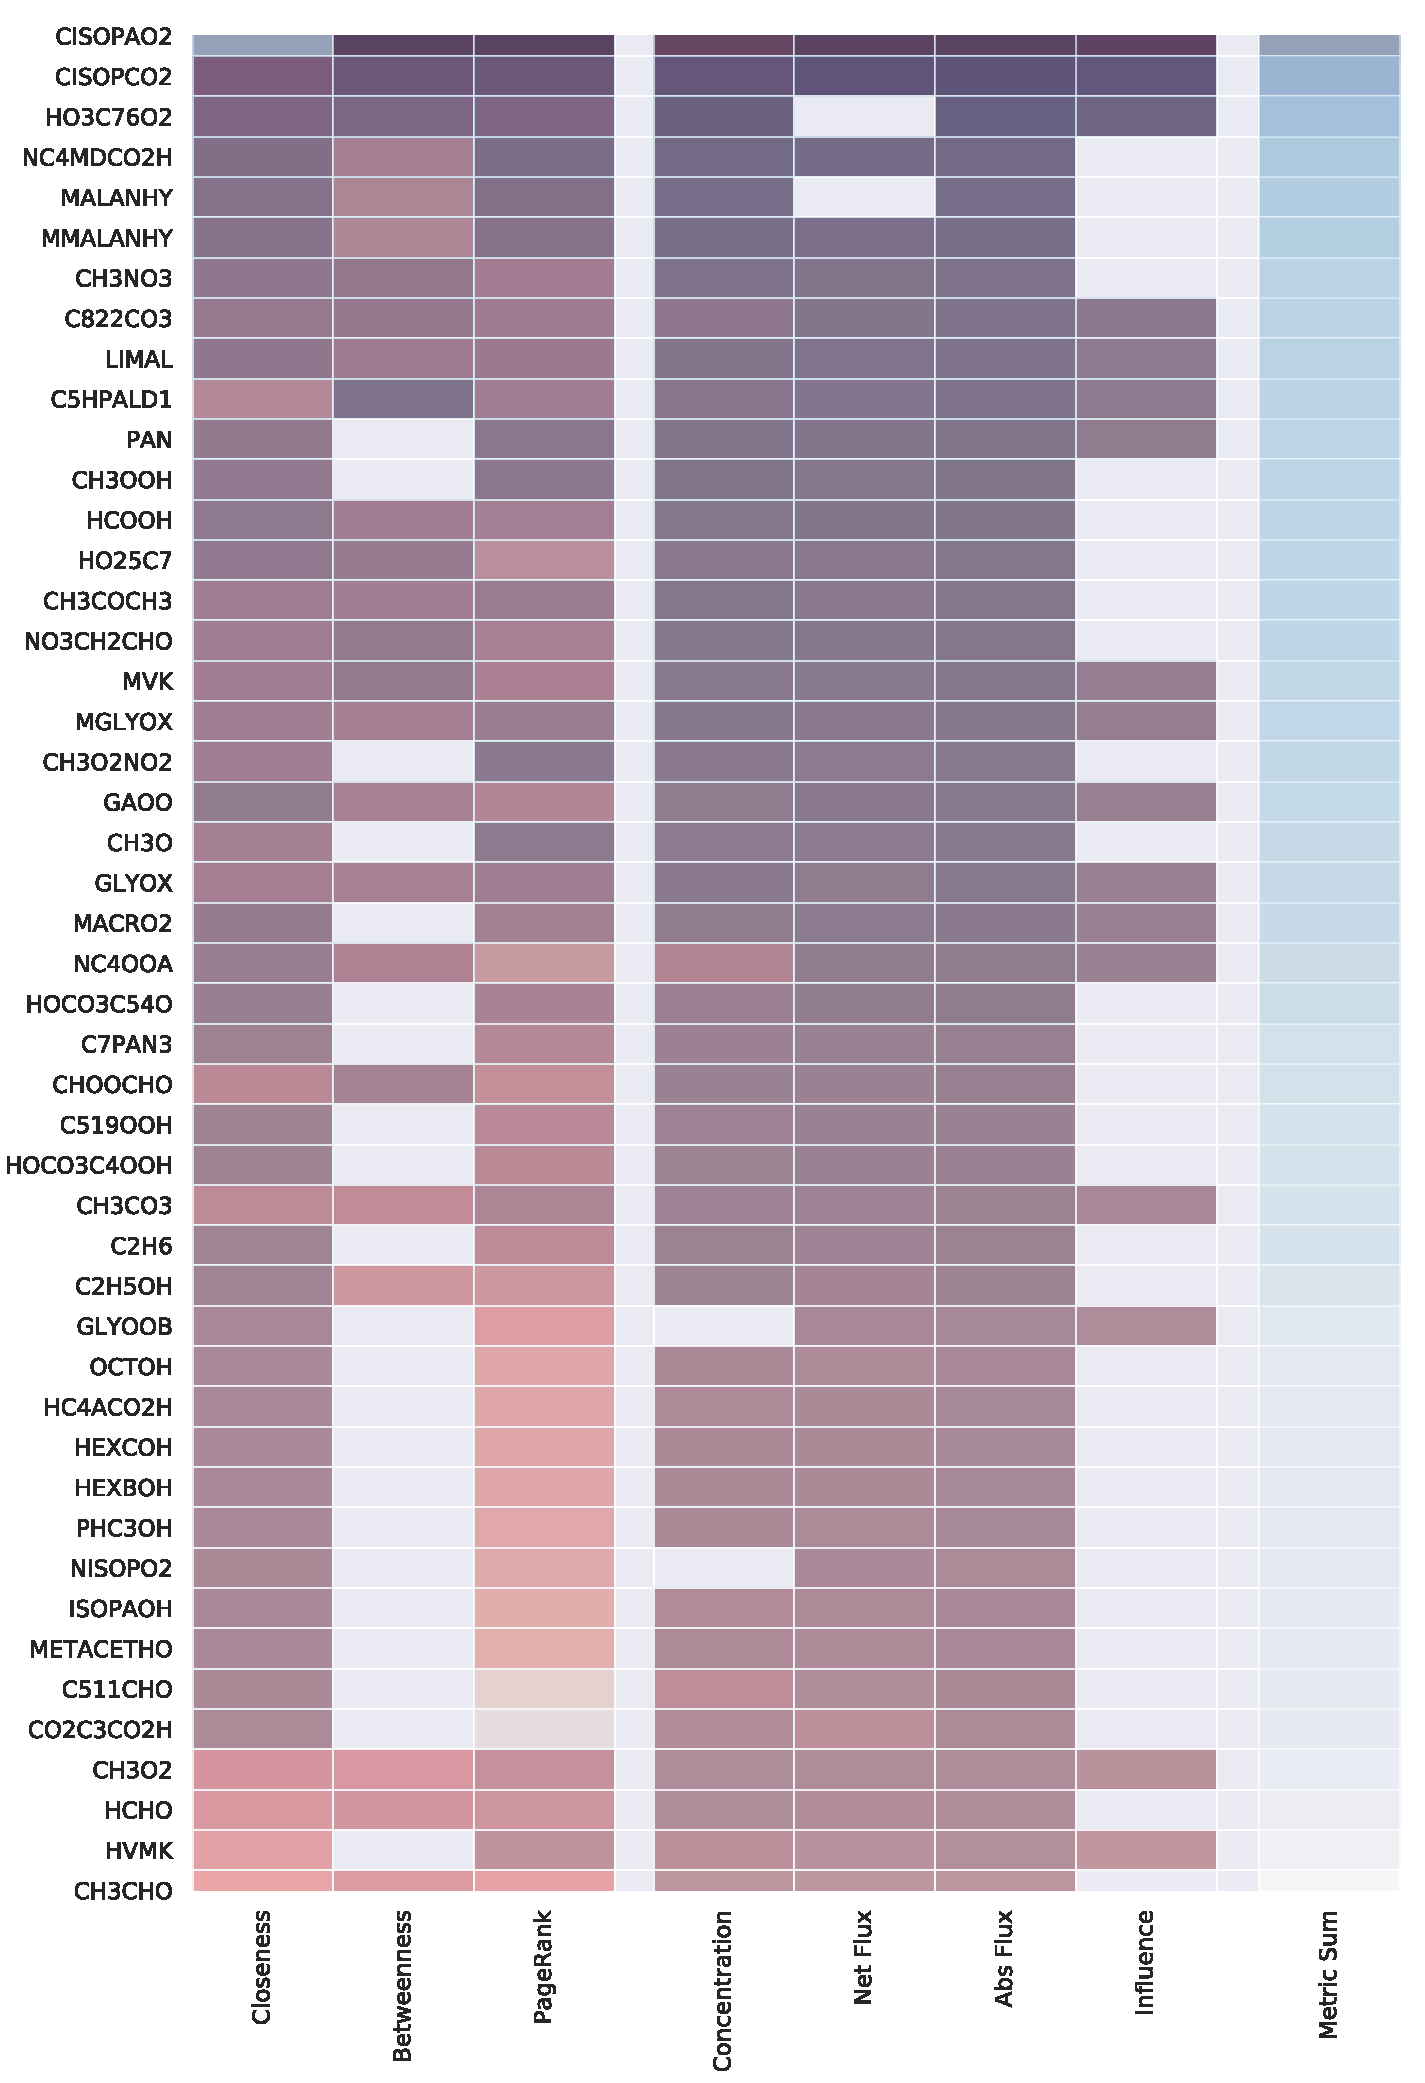
\includegraphics[width=.95\textwidth]{figures_c3/mlpregressor/aphh_Beijing.pdf}
        \caption{ \textbf{A bivariate heatmap comparison of Beijing.} }
        \label{fig:heatbj}
\end{figure}



%
%

\subsection{Providing An Overall Overview Using The TF-IDF And The Metric Sum.}
In the previous section, it was shown that centrality metrics could be used to complement the use of traditional metrics in the analysis of the chemical network. As each metric represents a different aspect of importance, should a single ranking value for a node be required, it is possible to take the average sum of all three metric values. Looking at \autoref{fig:heatbj} it is possible to see similar trends in colour gradient between the purples of the traditional metrics of flux and concentration with the total metric sum (the blue column). This suggests that it is possible to compare each scenario with the use of the metric sum.

In selecting the ten highest-ranking species from the mean centrality metric table for each simulation, \autoref{tab:groupcomp} can be created. Unlike the previous method, we are now looking at species which are essential across all metrics in a simulation.
Beijing consists mainly of Quinones and Dialdehydes, which are both derivatives of Benzene. London again has Benzene related compounds, mixed with the fast photochemical indicators, which were also ranked highly in \autoref{fig:heatl}. Looking at the highest-ranking sum (NaN-mean), it is seen that Isoprene, hept/hexane and glyoxal products highlighted as the most consistently important across all four simulations.

\begin{table}[H]
\centering
\small
\begin{tabular}{llllll}
\toprule
{} &         London &         Cape Verde &           Beijing &           Borneo &          Nan-Mean \\
\midrule
0 &       \ {HCHO} &      \ {PBZQOH} &     \ {PTLQONE} &     \ {C622OH} &    \ {CISOPCO2} \\
1 &     \ {CH3CHO} &      \ {PHENOL} &     \ {PBZQONE} &     \ {C923OH} &    \ {CISOPAO2} \\
2 &  \ {C5CO14OOH} &  \ {C24O3CCO2H} &  \ {HOHOC4DIAL} &      \ {C54OH} &     \ {C517CHO} \\
3 &    \ {PBZQOOH} &    \ {NBZFUONE} &  \ {MNNCATCOOH} &    \ {HO2C4OH} &     \ {HO2C6O2} \\
4 &    \ {MALANHY} &  \ {TLBIPERNO3} &    \ {C6H5CO3H} &     \ {C624OH} &   \ {HCOCH2CO3} \\
5 &     \ {CH3CO3} &    \ {BZBIPERO} &    \ {EPXDLPAN} &     \ {HEXAOH} &      \ {C717O2} \\
6 &      \ {C57OH} &  \ {TLEMUCCO2H} &     \ {C5DIALO} &   \ {C822CO2H} &   \ {HCOCOHCO3} \\
7 &    \ {C624CHO} &  \ {BZEMUCCO2H} &    \ {NBZFUOOH} &  \ {MACROHOOH} &  \ {HOCH2CH2O2} \\
8 &      \ {GLYOX} &       \ {PTLQO} &  \ {TLBIPEROOH} &  \ {HO14CO2C4} &   \ {HOC2H4CHO} \\
9 &  \ {HCOCOHCO3} &    \ {NNCATECO} &    \ {NCRESOOH} &   \ {C624CO2H} &     \ {C626CHO} \\
\bottomrule
\end{tabular}
\caption{\textbf{A table of the top 10 ranked species for each simulation.} Only species that exist within at least 3 out of the four simulations are used. The Nan-Mean takes the mean of all available data, ignoring runs where a species is not present. Species presented within the table follow the MCM naming convention.}
\label{tab:groupcomp}
\end{table}



\textit{\textbf{A note on finding the precursors}\\ Graphs are also useful in the back navigation of a network. It is possible to discover the most probable primary emitted species (nodes with no in-degree) by comparing the shortest path lengths for all primary emitted species (not including inorganic species). Here the primary emitted species with the smallest number of connections are often the most likely source.}




\section{Causality Analysis using the Jacobian and Pagerank}

Due to the complex inter-dependency on species within an atmospheric network, it is often hard to calculate how much of an effect perturbing one species will have on another. Classically we can find the instantaneous change at a specific point in time by close examination of the Jacobian matrix - also known as the connectivity method.
Here \cite{connectivity} states that the value $J_{A, B}$ of a log-normalised Jacobian represents the effect changing a species A will have on species B - allowing us to determine a set of important species with an aim (e.g. mechanism reduction).

If we take the sum of all items in the B column ($\sum_{i \ne B} J[i, B]$) we can calculate the total production of species B. Expanding this method we can calculate the percentage importance of B's precursors. Here the species with the highest values present the most significance to the formation of B. If we were to look at the rows instead of columns, a similar analysis may be executed for a species loss. It is for this reason that in preparing the Jacobian for use within a graph, we take the net difference between production and loss contributions to determine edge direction and weight. 

\subsection{Source Analysis using PageRank}
The PageRank value of a species can be calculated through the solving of eigenvalues and eigenvectors of a google matrix, or propagating a vector of unity through the network in small increments (Equation \autoref{eqn:forwards}). These solutions are both very similar to the integrator we use to propagate the chemistry within our box model - where instead of concentration we move `information' between nodes in our network. 

This means that for a network of nodes \{A, B, C, D, E\} (\autoref{fig:forwardspr}) we can use page rank to determine where the flow of information ends up (ultimately E). However, if we are interested to find out how much each of these nodes contributes to the total amount of information gained by E, we need to look at the whole sequence in reverse. For a directed-graph, we may reverse the direction of the links (so that source $\rightarrow$ target becomes source $\leftarrow$ target) and then assign an arbitrary amount of information to our queryable node (E) and then propagate it forwards using page rank on our reversed network using the same edge weighting as before, \autoref{fig:backwardspr}. 


\subsection{Mathematical Equivalent of Edge Reversal}
The physical `flipping' of an edge direction is the most visually intuitive method reversing the direction, however, in \autoref{ch2} we discussed that the 2D relational data of a network may also be represented through the use of an adjacency matrix. Since this is a matrix of links where row elements $\rightarrow$ column elements, the reversal of these edges is mathematically identical to taking the transpose of the matrix. 

In terms of our chemistry, our network is derived using the net values of our second order, partial derivative, relational matrix - the Jacobian. This makes the link reversal procedure equivalent to transposing the Jacobian, and thus analogous to the creation of the adjoint. The adjoint matrix is often used within the modelling world, to run backwards in time and make historic predictions based on current data \citep{adjgeos}. This has its application in determining the geolocational source of pollution, or in our case the source of concentration change in a species of interest. 

\begin{figure}[H]
    \centering
\begin{subfigure}{.9\textwidth}
  \centering
  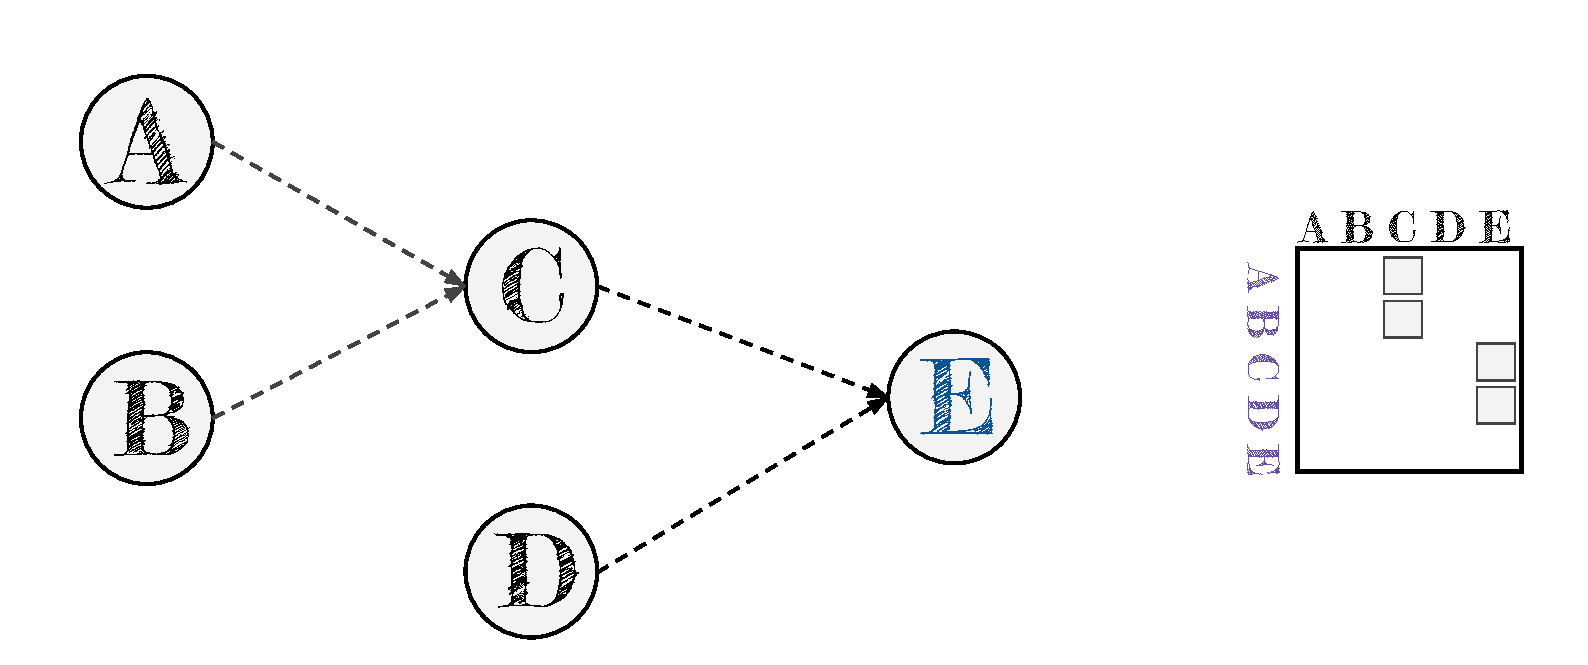
\includegraphics[width=\textwidth]{figures_c3/traditional.pdf}
  \caption{Traditional Influence Graph}\label{fig:forwardspr}
\end{subfigure}

\begin{subfigure}{.9\textwidth }
  \centering
  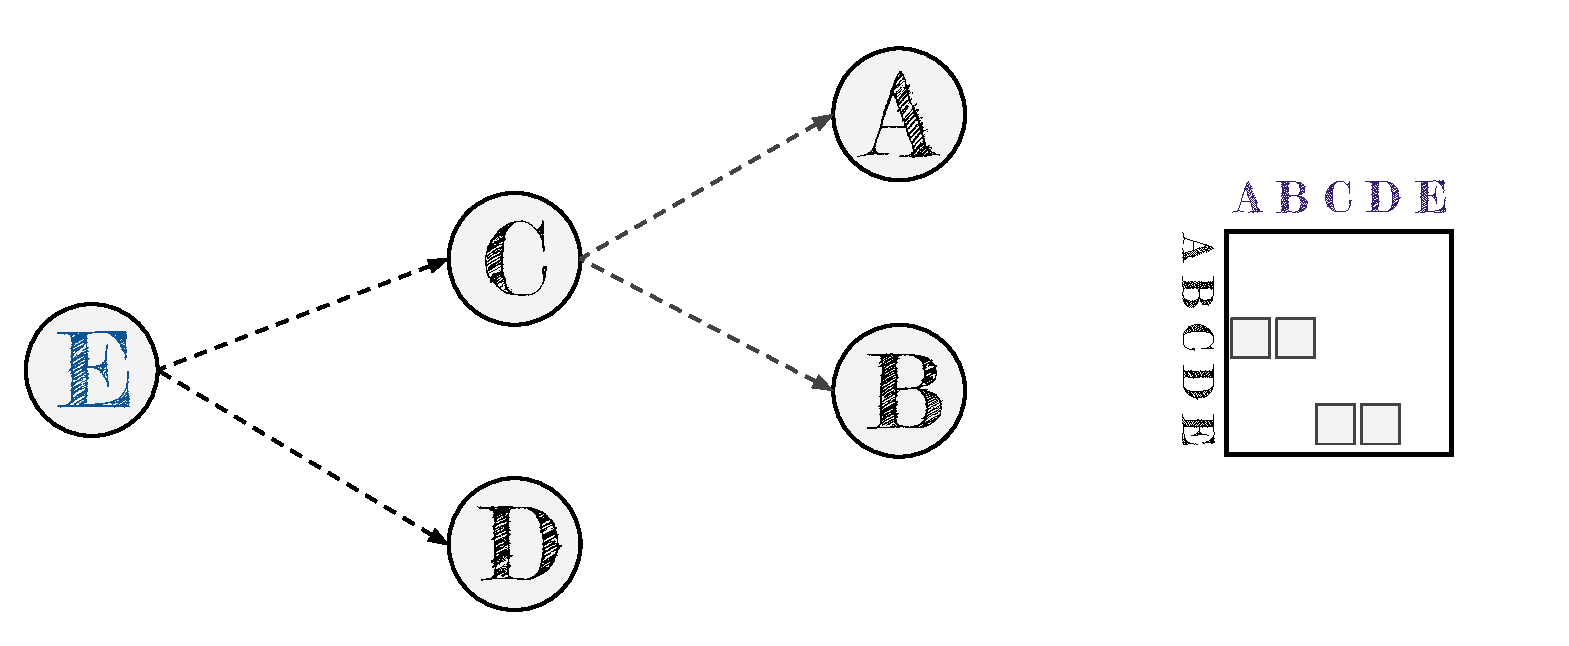
\includegraphics[width=\textwidth]{figures_c3/adjoint.pdf}
  \caption{Reversed-link (adjoint) influence graph}\label{fig:backwardspr}
\end{subfigure}

\caption{\textbf{Link reversal of the Jacobian Sensitivity matrix graph results in a graph of the adjoint.} Showing changing the direction of links in a graph is equivalent to applying the transpose to an adjacency matrix (right). In the case of a Jacobian based graph, this is analogous to using the adjoint to propagate the model back in time - something that can be used to identify the influence upon a species with a model.}
  \label{fig:prgraphs}
\end{figure}


\subsection{A Calculated Case Study}
To illustrate the points made within this section we select a species (MCM name: NC101CO) from a sample simulation of the MCM (Borneo initial conditions are given in \autoref{tab:icsmetric}). A brief mechanism analysis allows us to determine the precursors of \ch{NC101CO} by isolating its local sub-graph and reversing it. This is done by looking at outwards arrows in \autoref{fig:prtest1}. 




\begin{figure}[H]
  \centering
  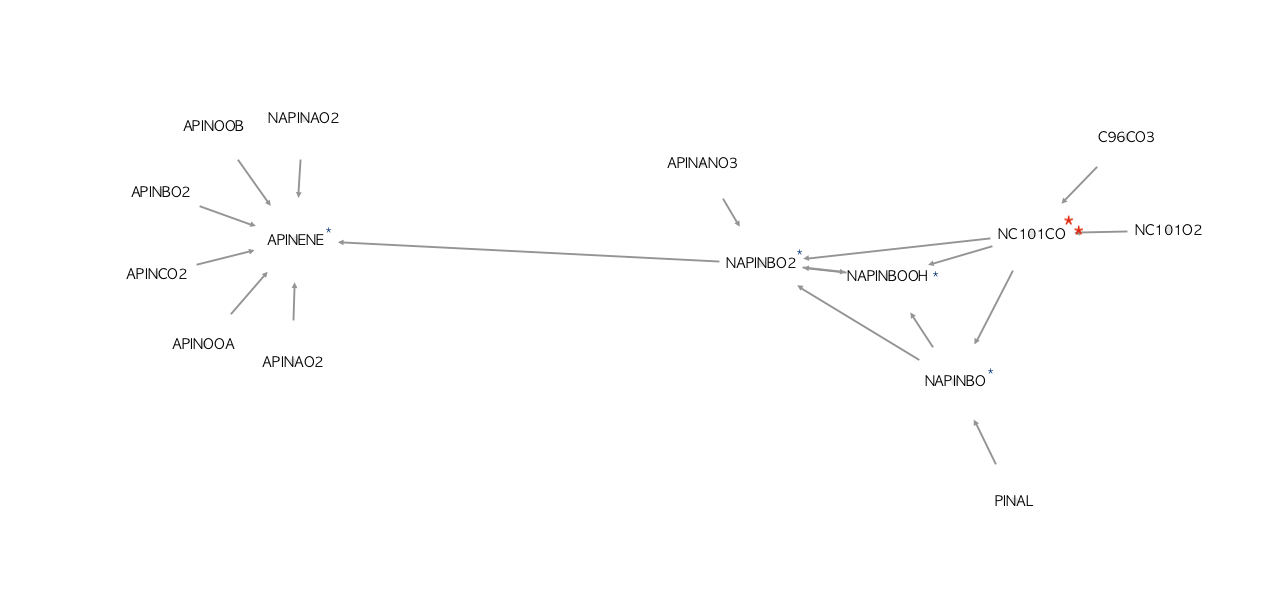
\includegraphics[width=1.1\textwidth]{figures_c3/prtest1.png}\\
  
  \begin{verbatim}
                              ! Sources of NC101CO
                                  NAPINBO-->NC101CO+HO2
                                  NAPINBO2-->NC101CO
                                  NAPINBOOH+OH-->NC101CO+OH

                              --- 2nd generation precursors ---
                              ! precursors of NAPINBOOH
                                  NAPINBO2+HO2-->NAPINBOOH

                              ! precursors of NAPINBO
                                  NAPINBO2+NO-->NAPINBO+NO2
                                  NAPINBO2+NO3-->NAPINBO+NO2
                                  NAPINBO2-->NAPINBO
                                  NAPINBOOH-->NAPINBO+OH

                              ! precursors of NAPINBO2
                                  NAPINBOOH+OH-->NAPINBO2
                                  APINENE+NO3-->NAPINBO2

                              --- 3rd generation precursors ---
                              ! APINENE is a primary emitted species
  \end{verbatim}

\caption{\textbf{The reversed subgraph between $\alpha$-pinene, and NC101CO.}\\ This is a subgraph showing the production of \ce{NC101CO}. Arrows point towards a species precursor. }
\label{fig:prtest1}
\end{figure}

\subsubsection{Personalised PageRank}
Using the reversed network we apply a `personalised' version of PageRank. This means that we initiate NC101CO with a ranking vector of 1000000 and -1 for all other species. A damping factor of 0.01 is also used within the algorithm to produce the results in \autoref{tab:nc101}. As is often seen within the algorithm, top-scoring values often have a notable split from mid and lower scoring values. We find that NC101CO has the strongest influence on itself (it is where we start our information), followed that of $\alpha$-pinene - its primary emitted precursor. Other influences such as NAPINBOOH, NAPINBO, \ch{NAPINBO2} are seen,  where NAPINBO has twice the influence from the others. This is most likely as this has the highest net-flux from the model (\autoref{tab:nc101vdot}).

\begin{table}[H]
\centering
\begin{tabular}{p{.6\textwidth}p{.2\textwidth}}
\toprule
Species & PageRank Ranking\\ \midrule
NC101CO   &  9.920000e-01 \\
APINENE   &  9.210000e-06 \\
NAPINBO   &  4.540000e-03 \\
NAPINBO2  &  2.770000e-03 \\
NAPINBOOH &  2.690000e-03 \\
\midrule
C511OOH   & -9.990000e-07 \\
C527NO3   & -9.990000e-07 \\
\bottomrule
\end{tabular}
\caption{A reversed graph Page Rank test with \ce{NC101CO}}
\label{tab:nc101}
\end{table}

\begin{table}[H]
\centering
\begin{tabular}{p{.6\textwidth}p{.2\textwidth}}
\toprule
Species & $\dot{v}$ (net flux)\\ \midrule
NAPINBOOH &     -0.458271\\
NAPINBO   &  -1840.391917\\
\ch{NAPINBO2}  &     -0.037366\\
\bottomrule
\end{tabular}
\caption{The net flux of the three species: NAPINBOOH, NAPINBO, \ch{NAPINBO2},\\ taken from a simulation of Borneo at 2020-06-24  12:09:56 }
\label{tab:nc101vdot}
\end{table}


\subsubsection{Iterative Analysis of the Jacobian}
 The total production of a species was also calculated by taking the sum of all items in the corresponding column (not including the diagonal), \autoref{tab:nc101jac}. As we are ignoring the diagonal\footnote{The diagonal of a Jacobian tells us the net change of a species, which can also be calculated as the difference of the column and row sums.} the first generation influence matches that of the reversed page rank algorithm. To get the total influence however we now have to repeat the process for each of the species producing NC101CO, and so forth. This process is identical to the iterative sum of in-degree links going backwards through our jacobian derived network - a process visually illustrated within \autoref{fig:backtrace}.

\begin{table}[H]
\centering
\begin{tabular}{p{.6\textwidth}p{.2\textwidth}}
\toprule
$J_{precursor -> NC101CO}$ & Value \\
\midrule
\ce{NAPINBO -> NC101CO}  &    47123.629418 \\
\ce{NAPINBO2 -> NC101CO}  &       0.000014 \\
\ce{NAPINBOOH -> NC101CO}  &      0.000001 \\
\bottomrule
\end{tabular}
\caption{The influence on \ch{NC101CO} from other species,\\ taken from a simulation of Borneo at 2020-06-24  12:09:56 }
\label{tab:nc101jac}
\end{table}








\subsection{Verdict}
As the PageRank algorithm is applied to the whole network and contains teleportation, it provides small values for species without a direct link to the species in question. This requires some sort of changepoint analysis to filter. 

A better method would be the calculation of the shortest simple path between a species in question and all other species, and then subtract the value obtained within each step to get its contribution. For the example \ce{A ->[4] B  ->[6]C} the shortest path from A to C would be ten and B to c would be 6. The influence of A on C  is calculated by the influence of A on B divided by the total influence on B. This is similar to the process required if we were to use the Jacobian Matrix directly. 

Overall, as we use the Jacobian matrix to create the graph, writing a script to process this may be the most computationally efficient (and comparable to other results). The graph representation and page rank methods may at first glance be quicker to implement, but do not necessarily produce numerical output that is immediately interpretable. They do however illustrate what the more traditional (mathematical) methods are doing in the background. Therefore both methods are equally difficult to implement, as well as being useful, and therefore it is up to the reader to select the one most appropriate to their aims. 





\section{Conclusions}

\autoref{ch1} and \autoref{ch2} explained the importance of visualisation and graph structure in communicating the complexity of an atmospheric chemical system. This chapter explores using a graph framework in cases where a network is too large or complex to represent visually.

We start by looking at several centrality metrics, which categorise nodes of importance within the network. Despite showing great promise in other fields, these do not seem to supply significant new insights into the chemical mechanisms of a model simulation when compared to traditional methods.

Next, we look at the classification of the MCM as a network. Here it is shown that this contains both small world and power-law features. This means that the network has both a local and global structure. The MCM network consists of a series of small `communities' of species which react with each other, connected by a hierarchical structure - a structure which can be utilised in the use of mechanism reduction (as seen in \autoref{fig:graphc1}).

\begin{figure}[H]
     \centering
     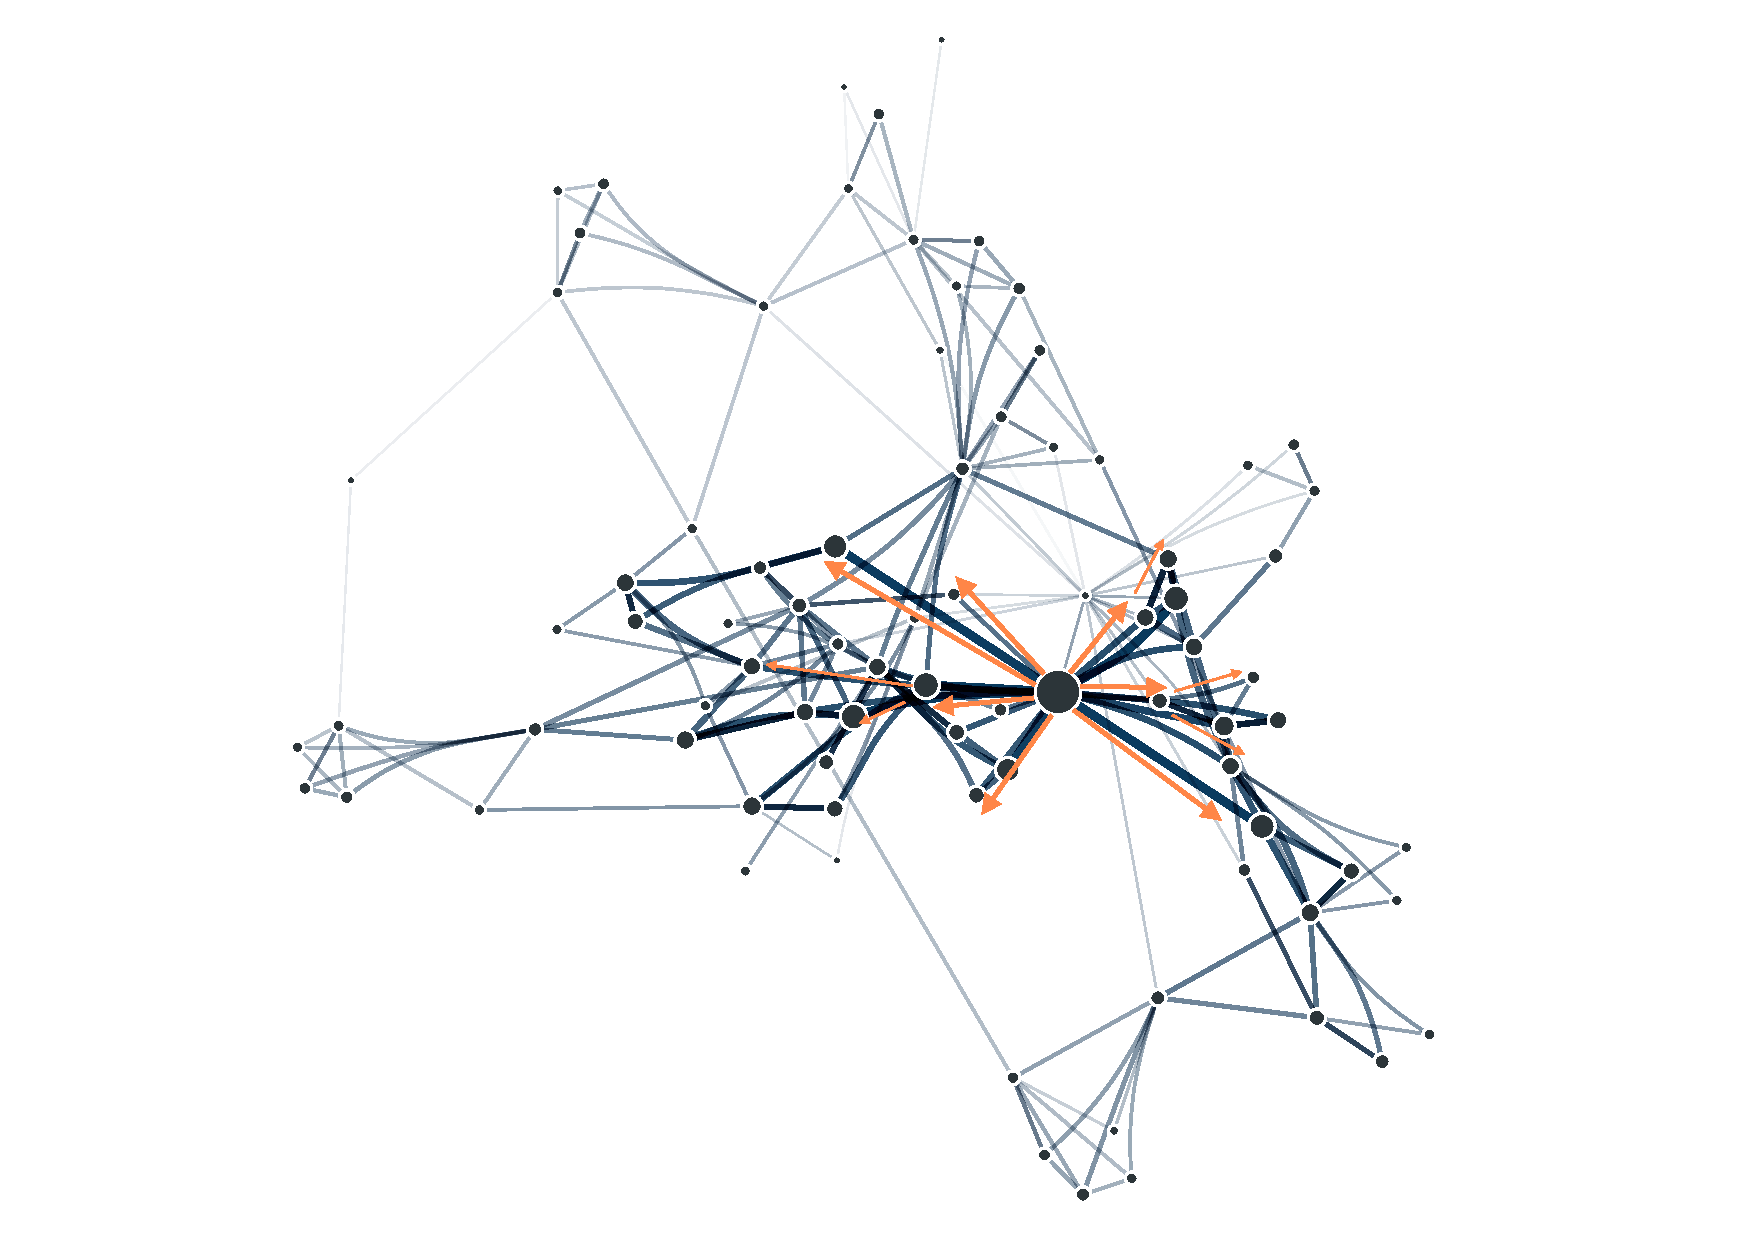
\includegraphics[width=1\textwidth]{newfigs/ch2_distance_links.pdf}
        \caption{\textbf{Showing total the influence from each species on HCHO for a sample MCM subset of Butane.} Species importance (node size) is determined using the reverse PageRank algorithm starting at HCHO (middle). It is calculated by taking a snapshot of a chemical simulation and rendered using the transpose of the Jacobian relational matrix. Link width is representative of the cumulative sum of the weights contributing to a concentration change of HCHO.  }
        \label{fig:backtrace}  
\end{figure}


Finally, it is possible to apply graph theory for the use of source analysis. Although this is analogous to manual matrix methods on the Jacobian, the use of a graph structure makes the explanation and understanding of the procedure more intuitive. Again there is no gain over the traditional Jacobian analysis methods.

To conclude, the graph-based analysis offers much of the same results as current methods. Since we do not obtain any new significant insight in applying these the new learning curve in embedding them into current practices of model analysis does not appear worthwhile. Instead, we further explore the modular structure of the MCM in \autoref{ch4}, where graph clustering techniques are applied to group species with a fast-flux between them.












%
